\chapter{Stellar Component}
	\label{cha:stellar}


The rest of this chapter is structured as follows: firstly we present the kinematic maps for the stellar component of the galaxy (section \ref{sec:stellarKin}) and a look at how they fit on the $\lambda_{R_e}$--ellipticity plane, then, in section \ref{sec:pop} we investigate the stellar populations using the absorption line strength. We conclude by looking at the odd-one-out of the sample NGC 612 in section \ref{sec:NGC612}

\section{Kinematics}
	\label{sec:stellarKin}

	\subsection{Maps}
		\label{subsec:maps}

		\begin{figure*}
      \centering
      \includegraphics[width=0.245\textwidth]{Vmaps/ngc0612_stellar_sigma.png}
      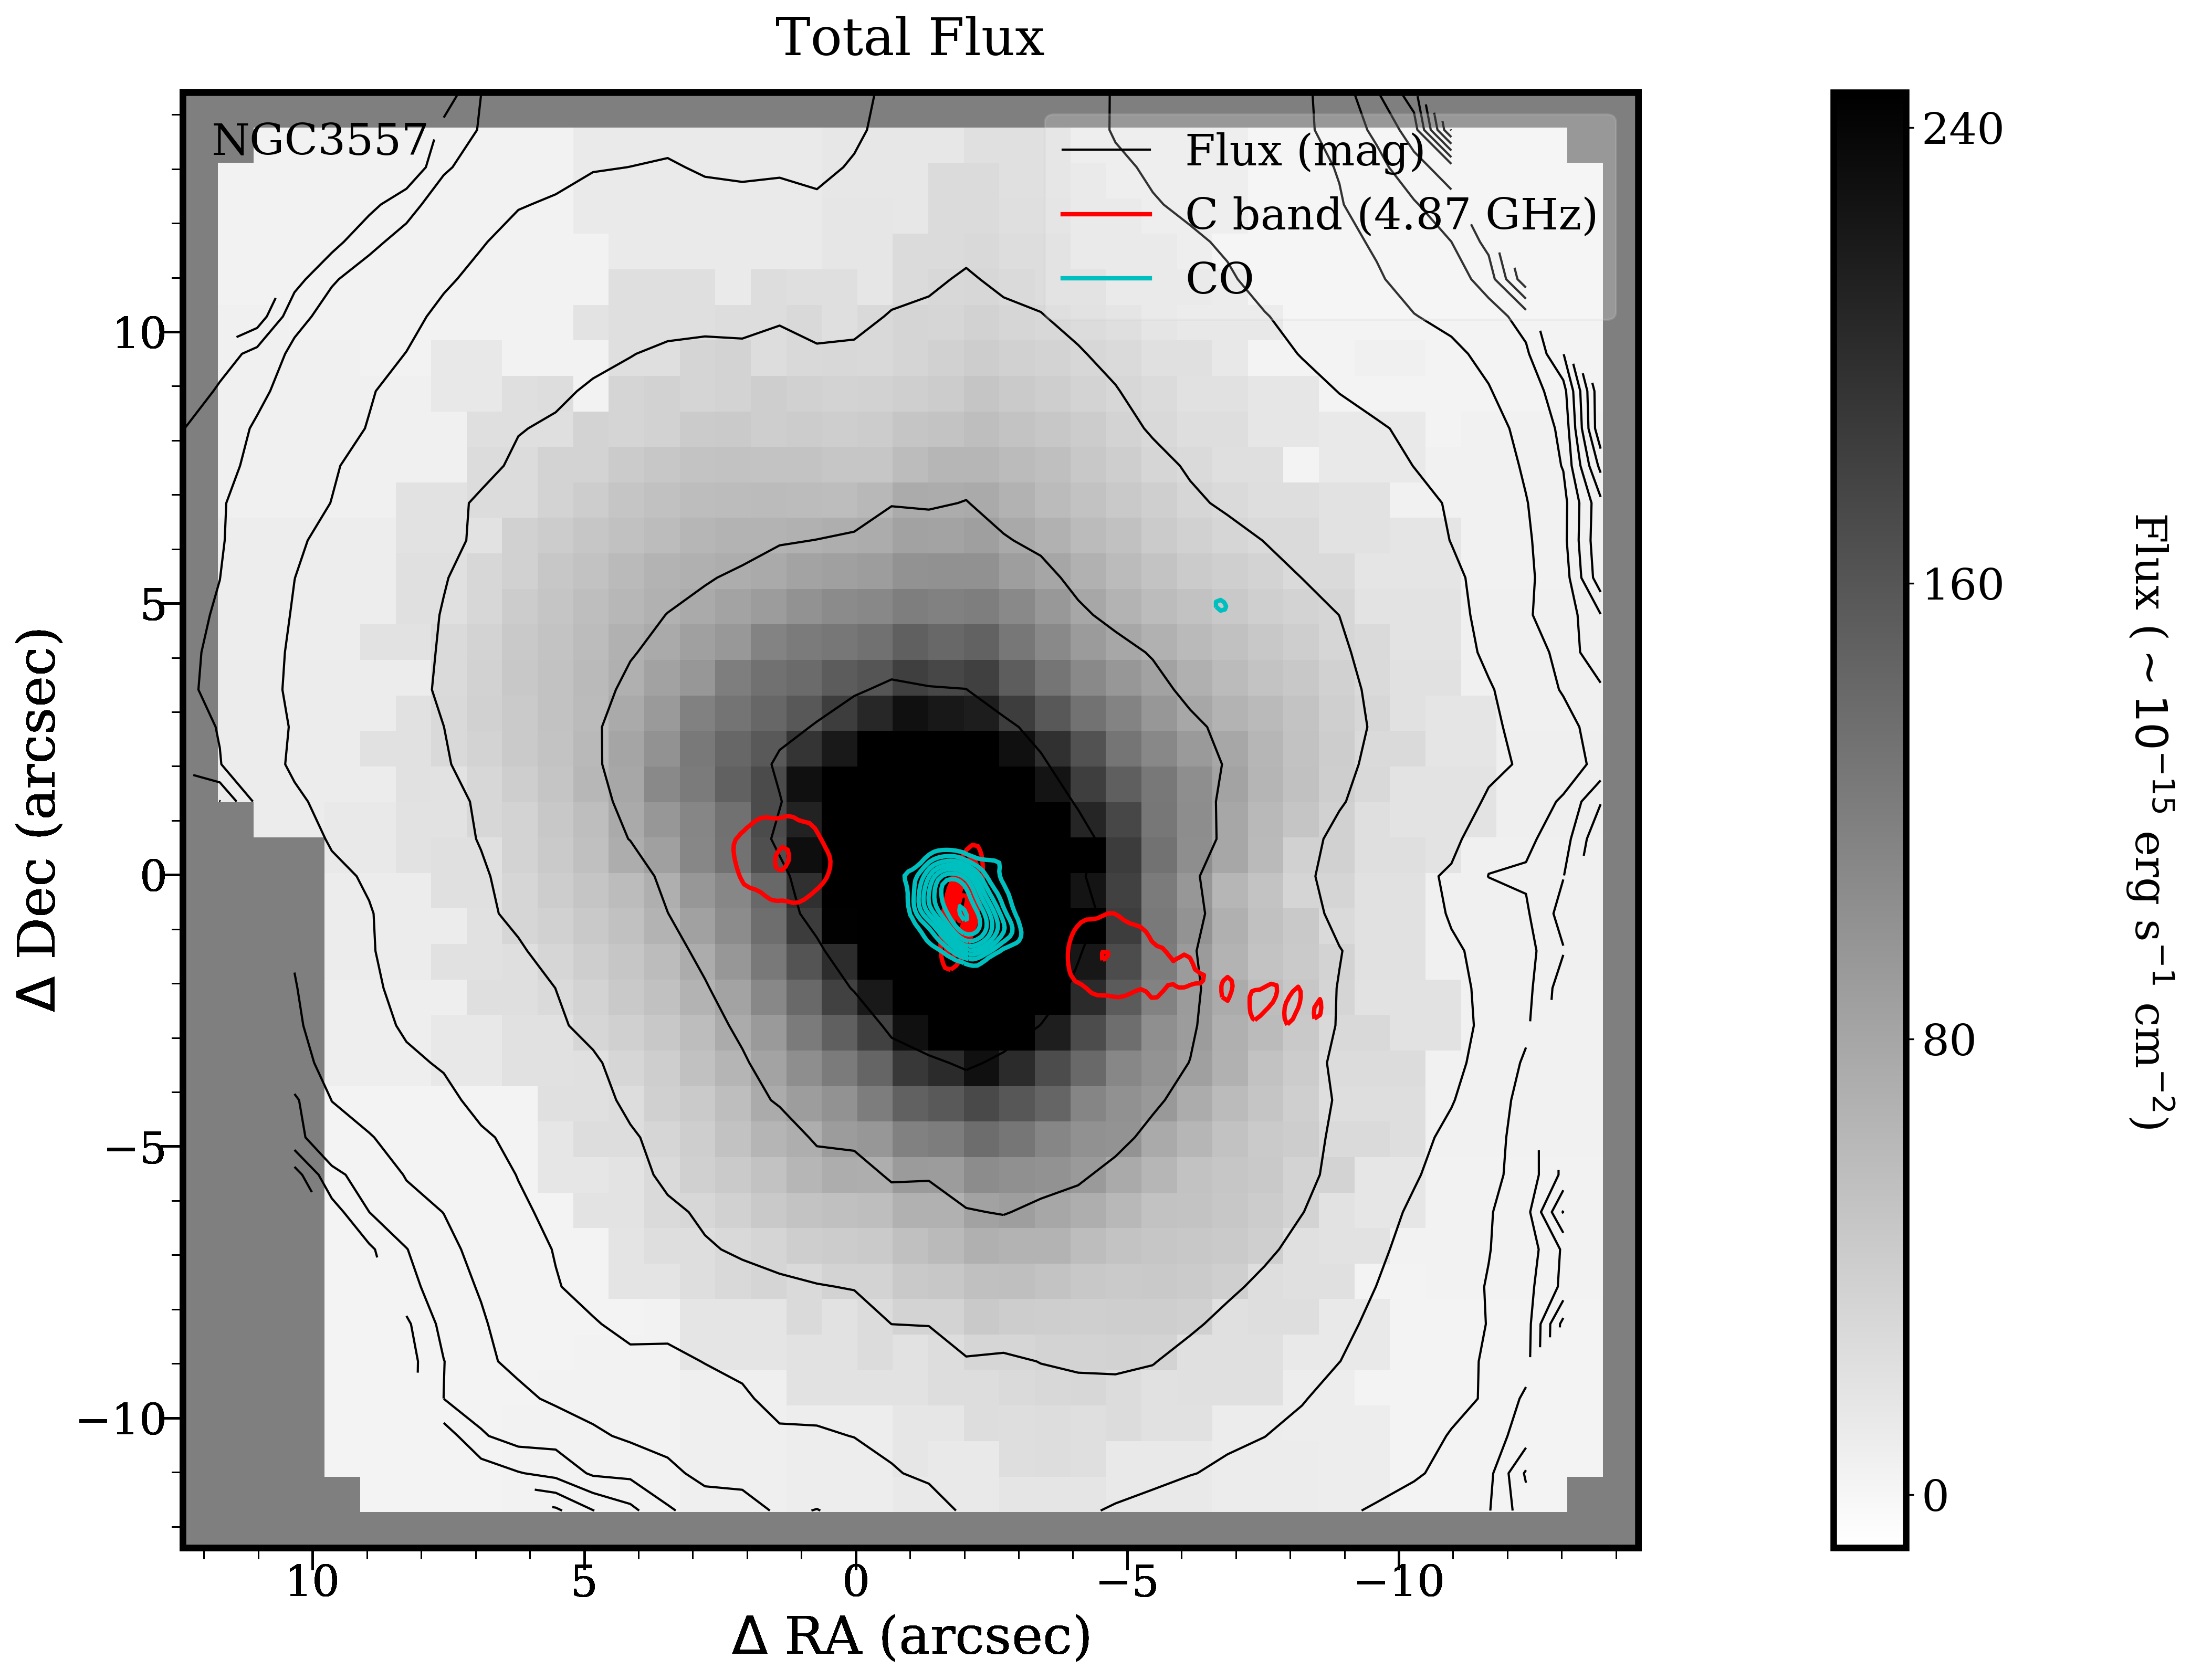
\includegraphics[width=0.245\textwidth]{Vmaps/ngc3557_stellar_img.png}
      \includegraphics[width=0.245\textwidth]{Vmaps/ngc3100_stellar_img.png}
      \includegraphics[width=0.245\textwidth]{Vmaps/ic1459_stellar_img.png}
      \includegraphics[width=0.245\textwidth]{Vmaps/pks0718-34_stellar_img.png}
      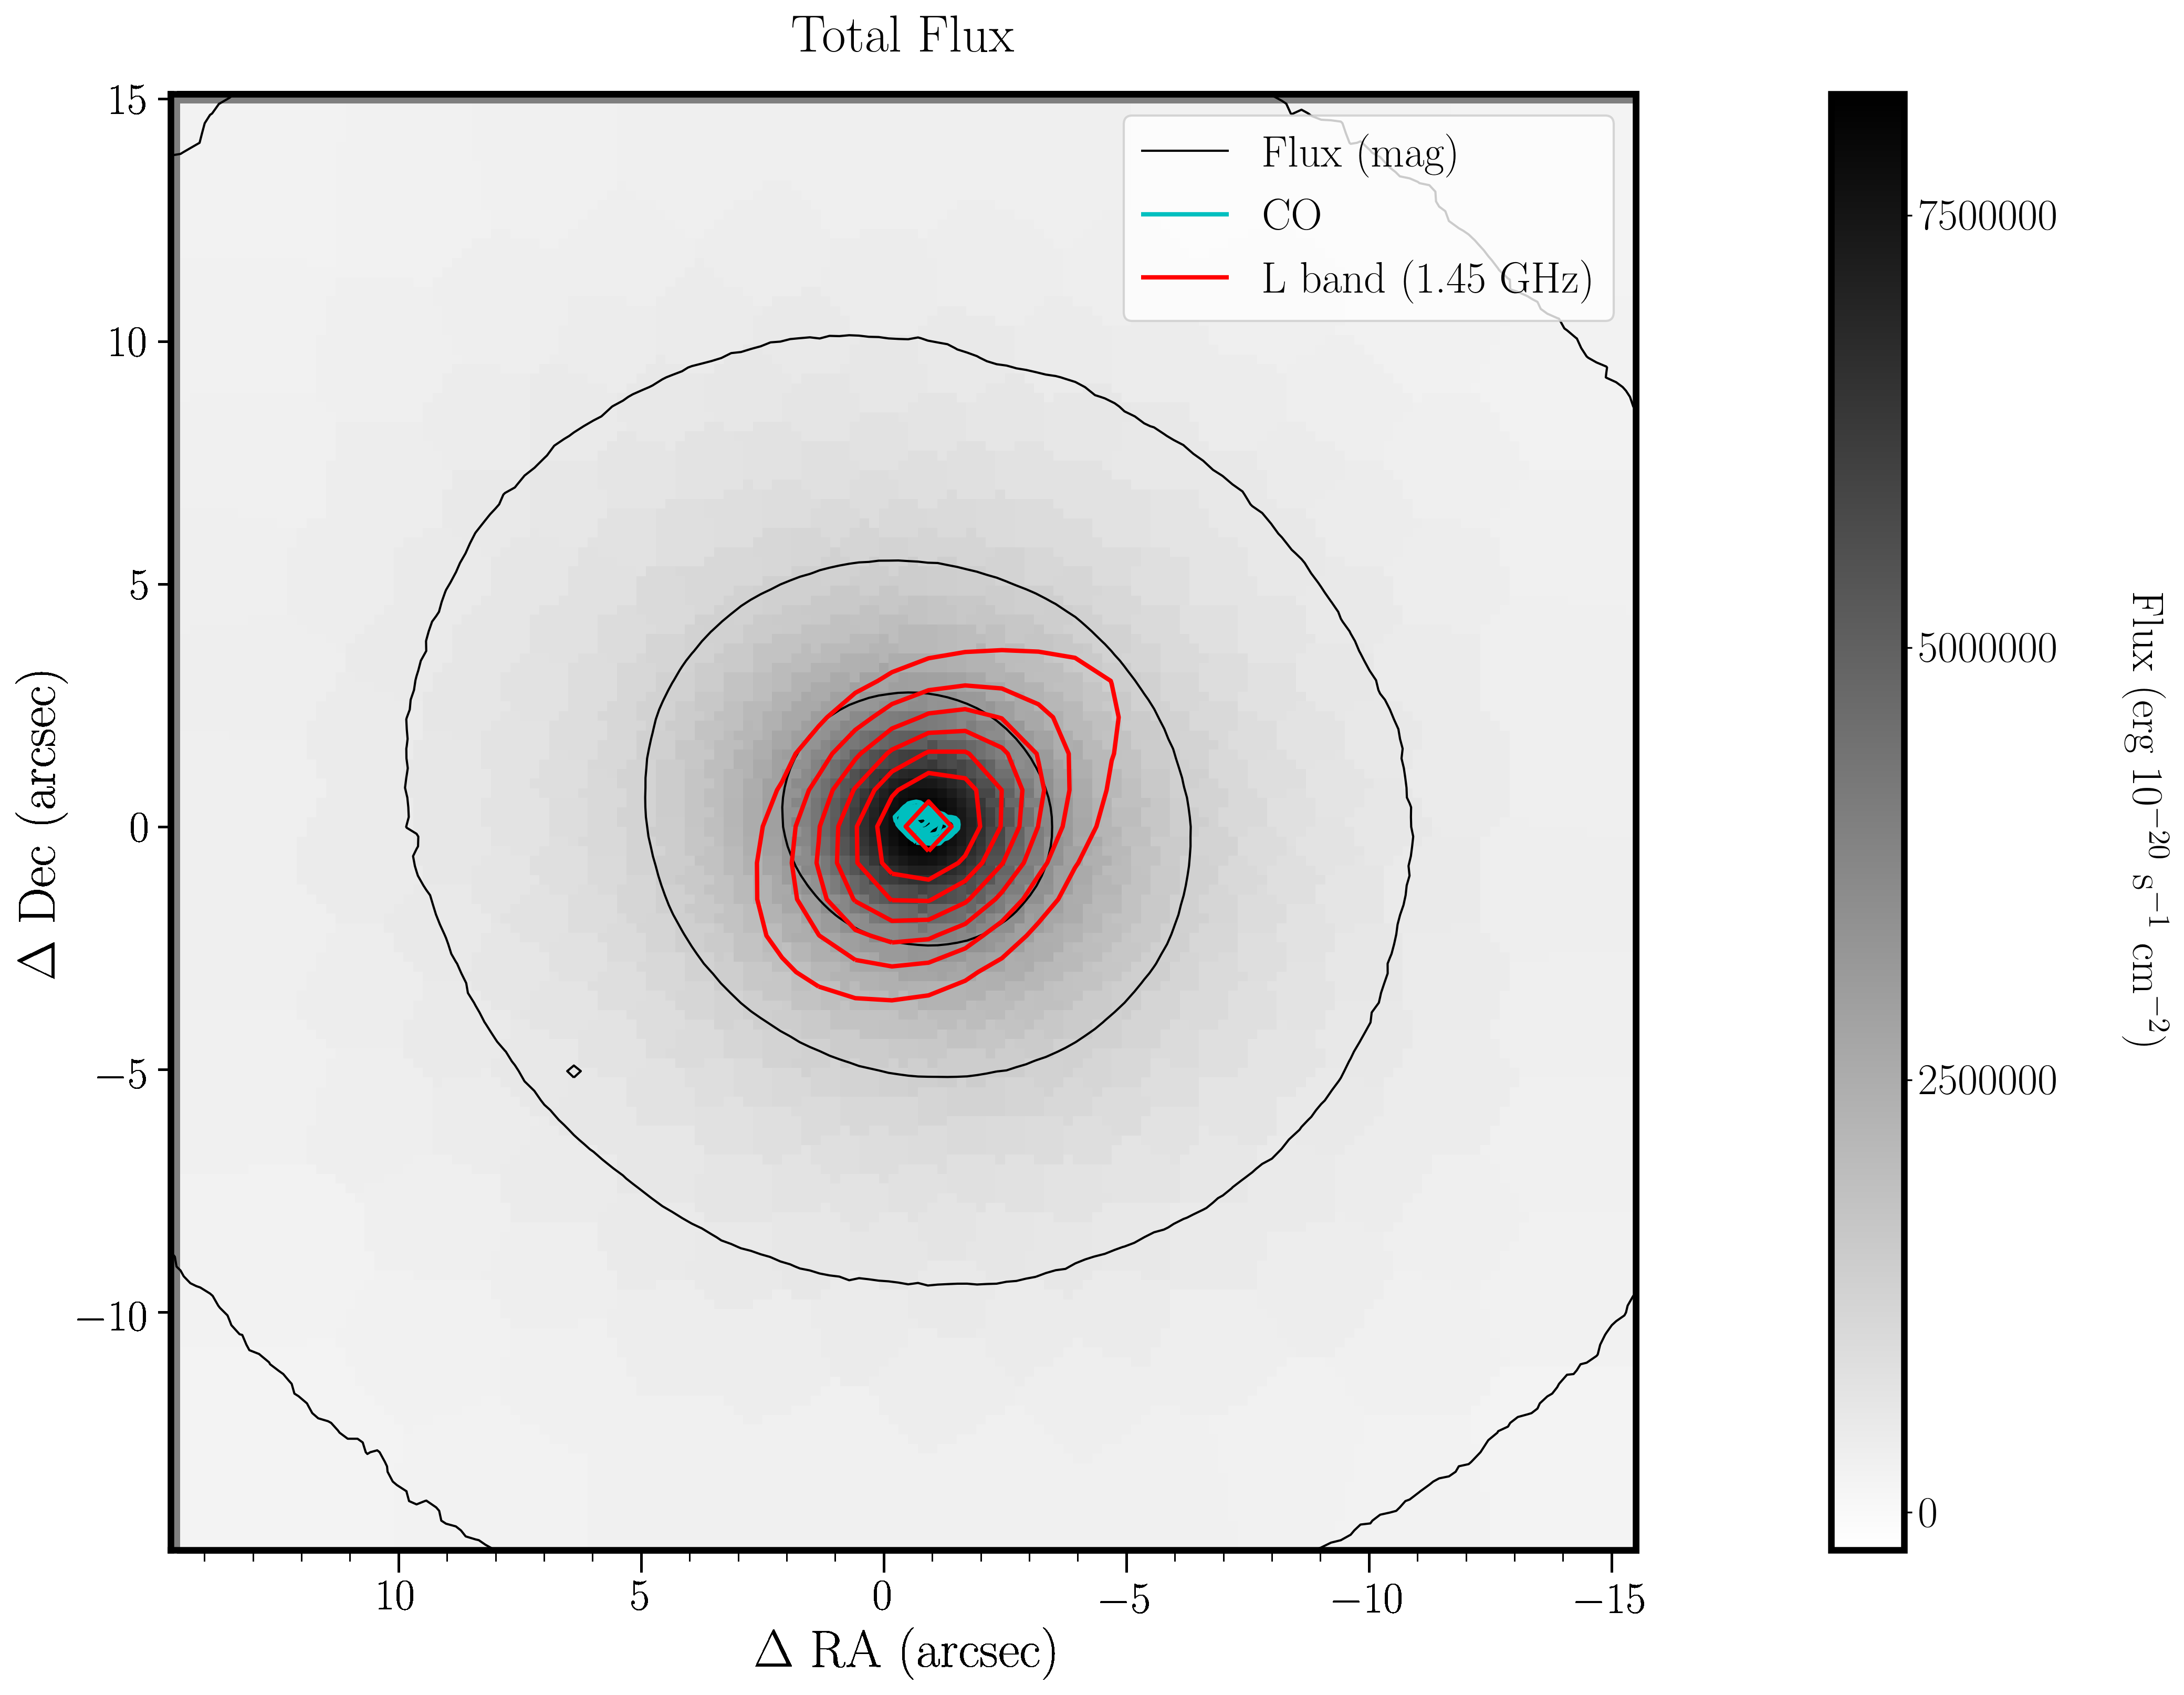
\includegraphics[width=0.245\textwidth]{Vmaps/ic4296_stellar_img.png}
      \includegraphics[width=0.245\textwidth]{Vmaps/ngc7075_stellar_img.png}
      \includegraphics[width=0.245\textwidth]{Vmaps/ic1531_stellar_img.png}
      \includegraphics[width=0.245\textwidth]{Vmaps/ngc1399_stellar_img.png}
      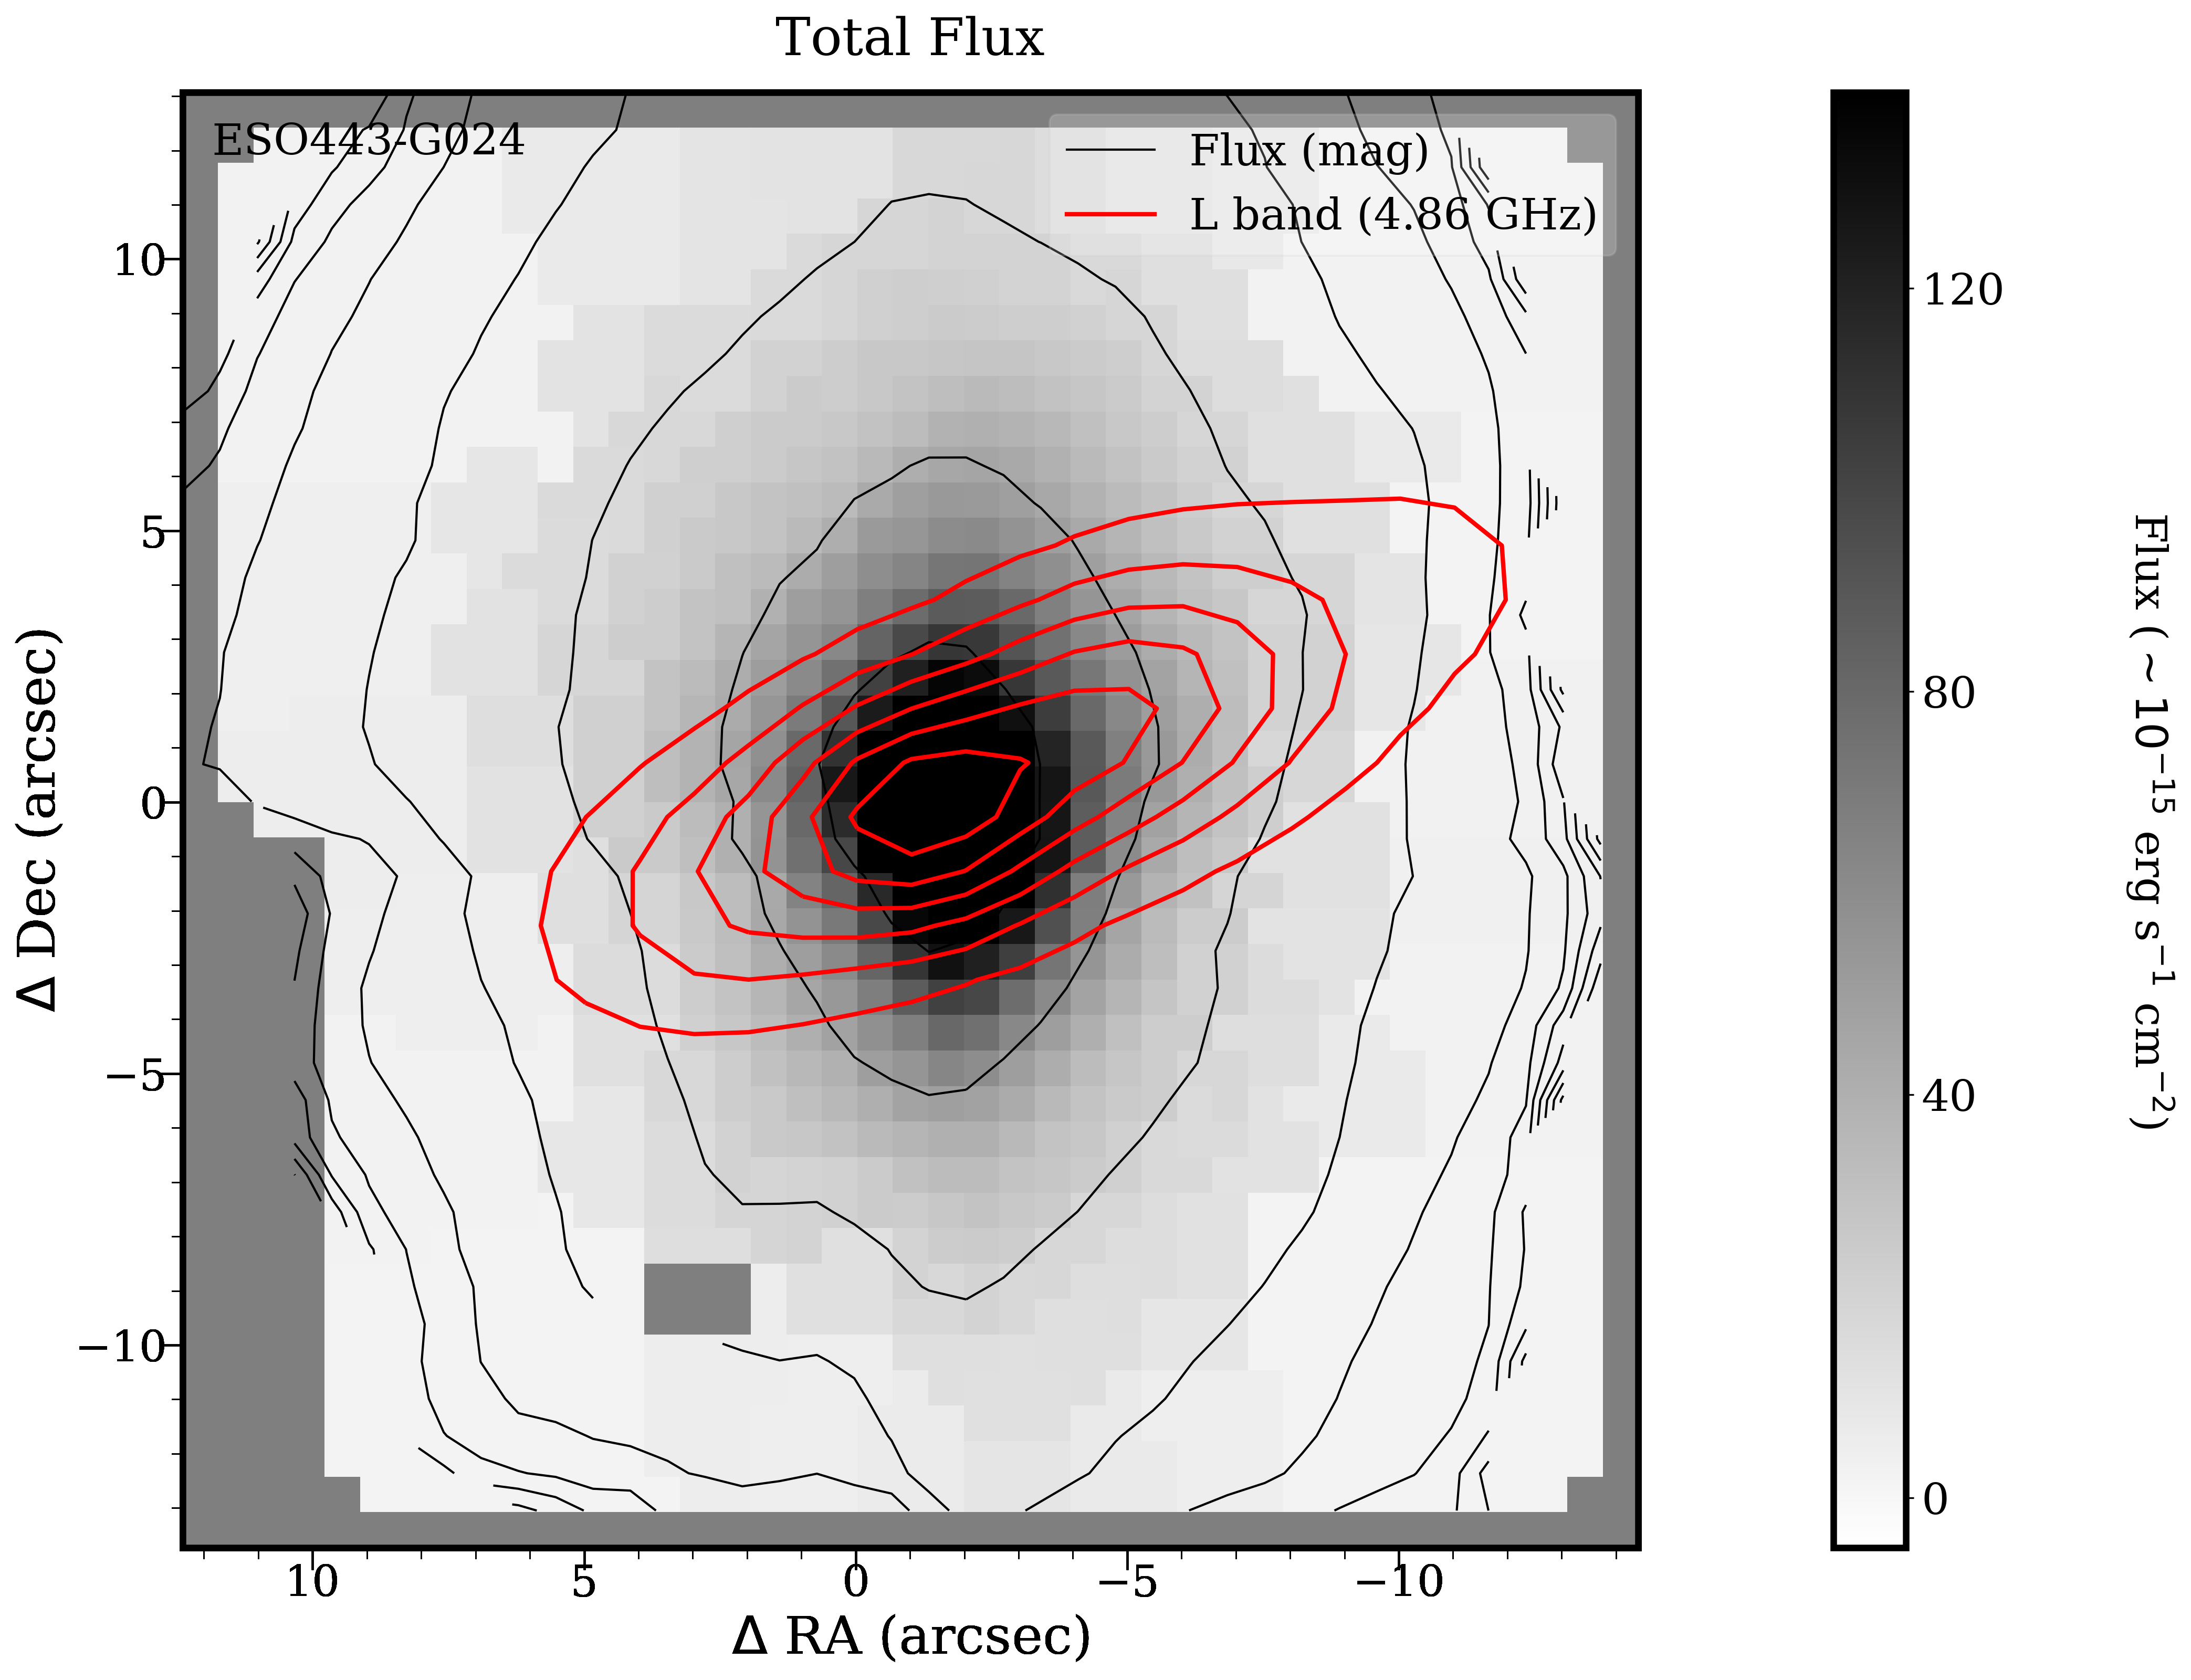
\includegraphics[width=0.245\textwidth]{Vmaps/eso443-g024_stellar_img.png}
      \caption[VIMOS images]{Image for each galaxy in the VIMOS sample. Plots are ordered roughly in peak stellar velocity, with flux contours in black, CO from ALMA in cyan and radio from VLA in red. The radio band displaied is shown in the legend of each plot and depends on what data is avaliable in the archive and which images had a similar resolution and and scale}
      \label{fig:Vstellar_img}
\end{figure*}

\begin{figure*}
      \centering
      \includegraphics[width=0.245\textwidth]{Vmaps/ngc0612_stellar_vel.png}
      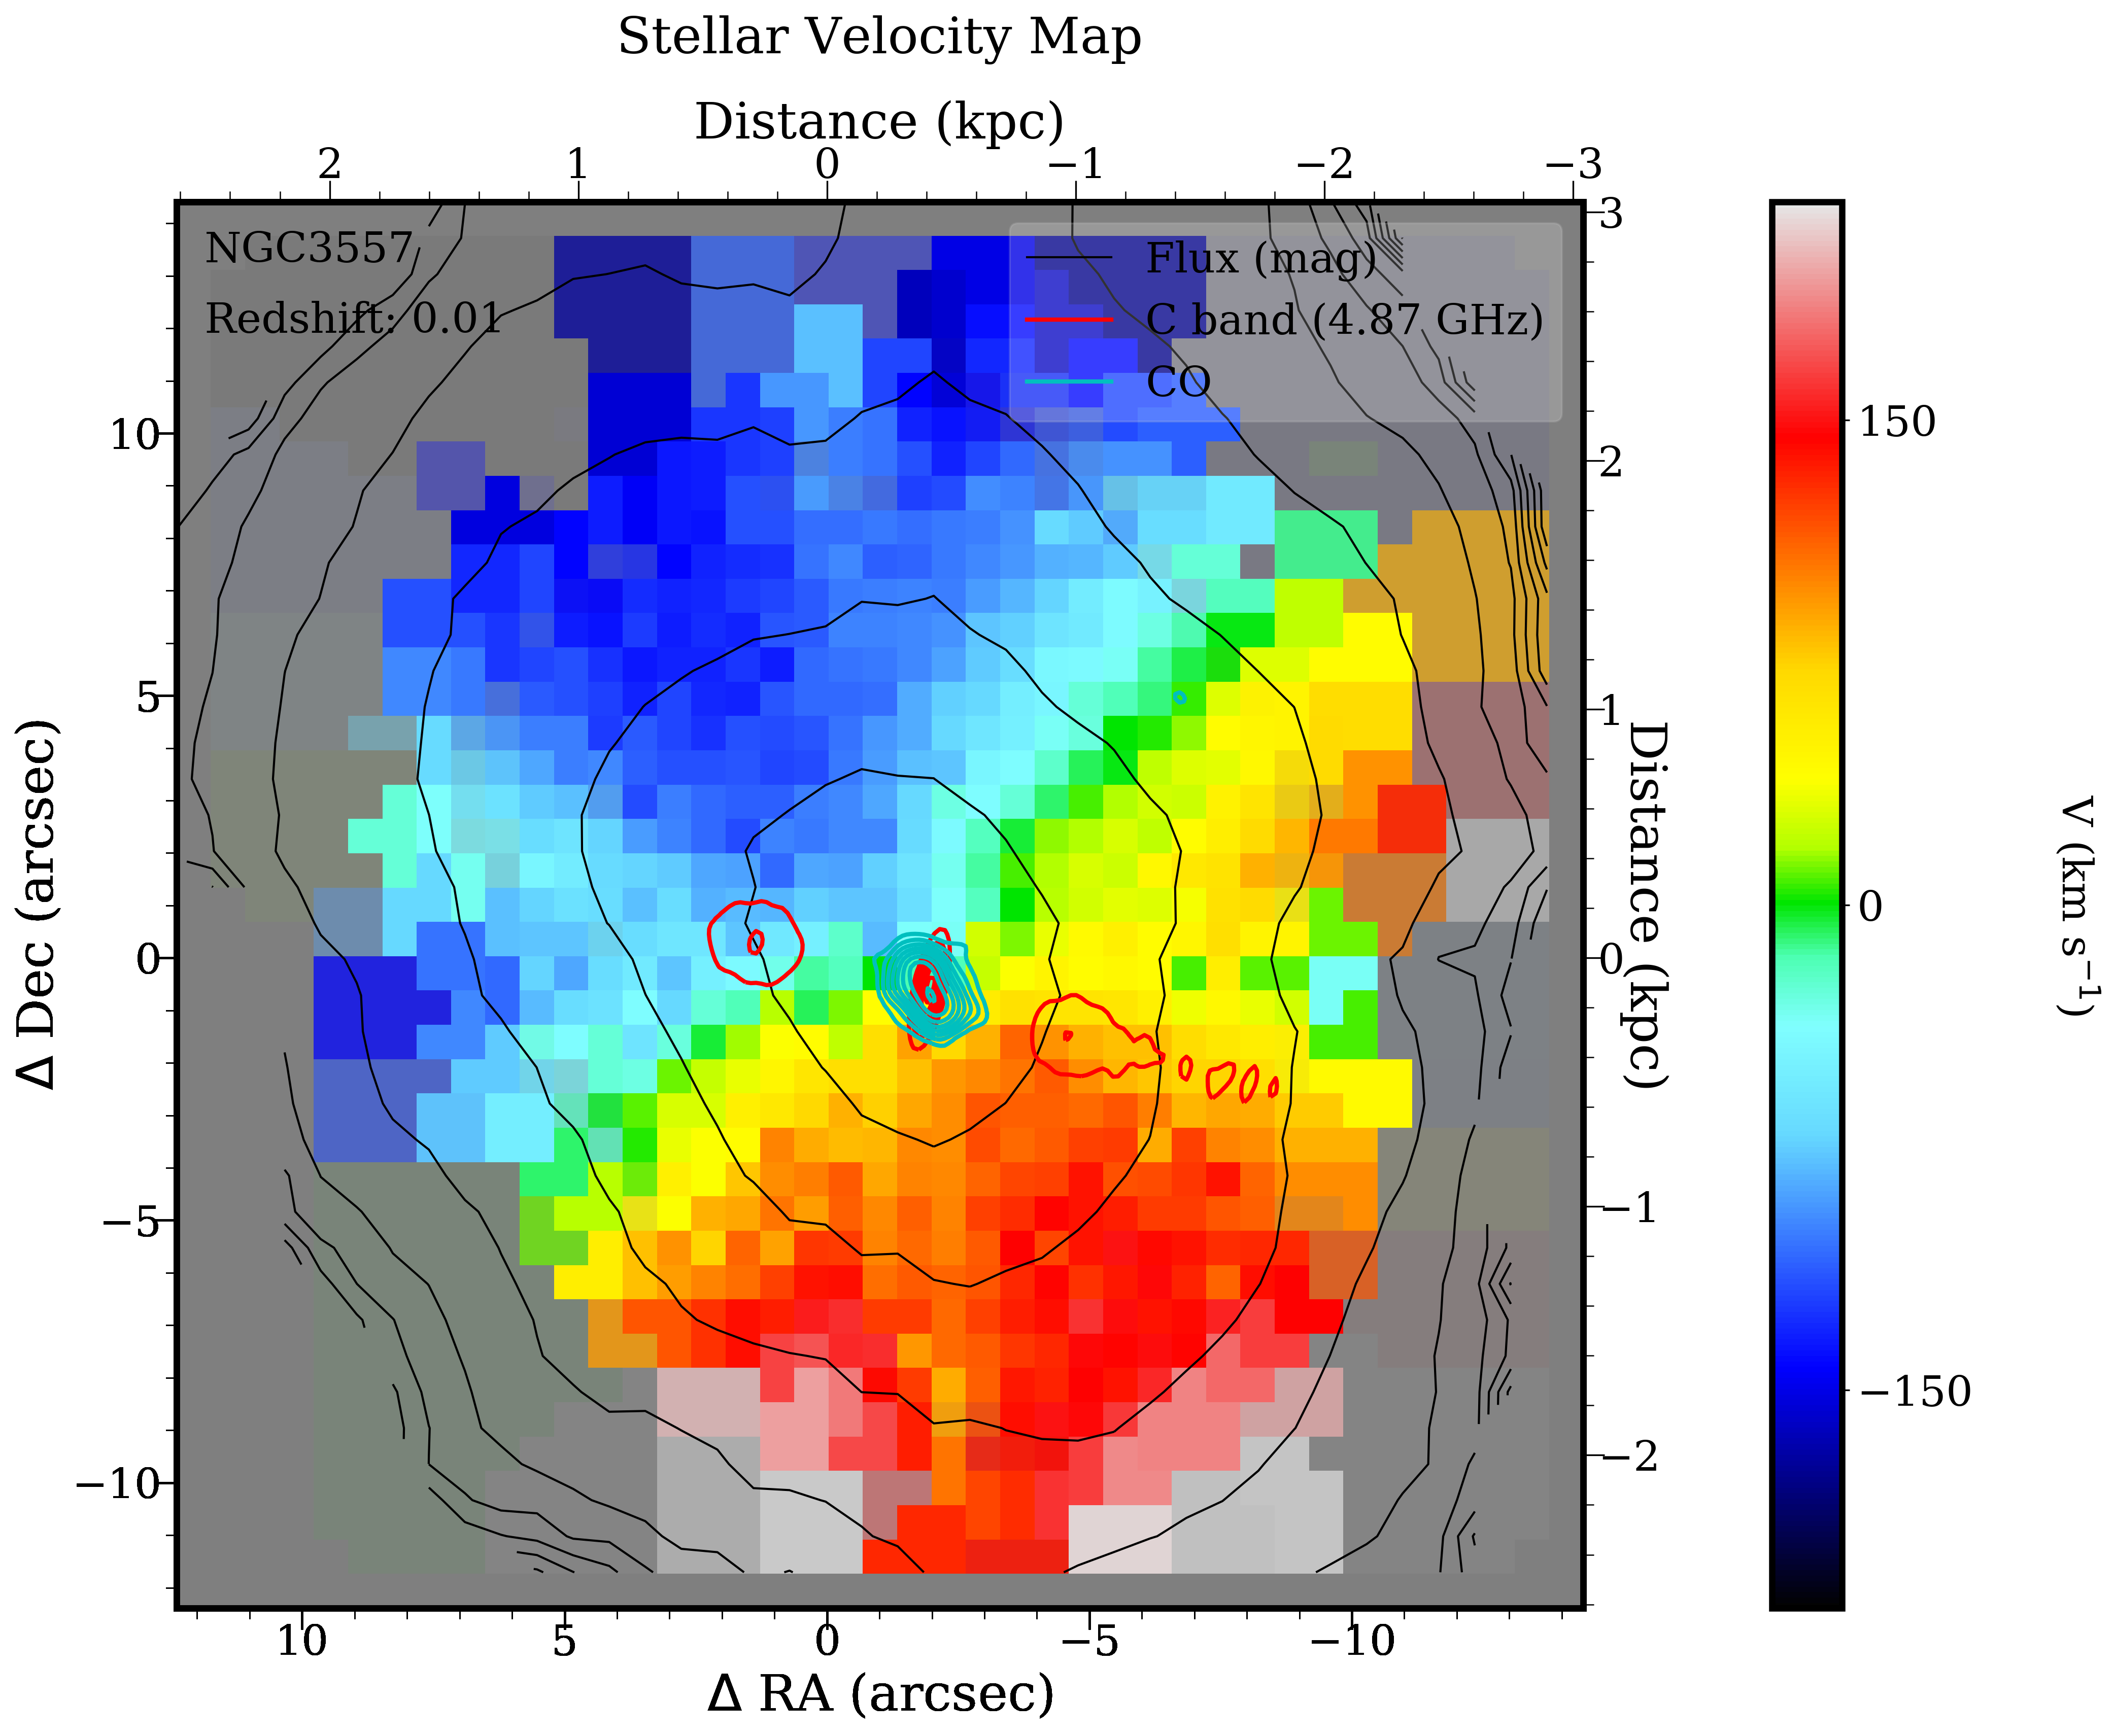
\includegraphics[width=0.245\textwidth]{Vmaps/ngc3557_stellar_vel.png}
      \includegraphics[width=0.245\textwidth]{Vmaps/ngc3100_stellar_vel.png}
      \includegraphics[width=0.245\textwidth]{Vmaps/ic1459_stellar_vel.png}
      \includegraphics[width=0.245\textwidth]{Vmaps/pks0718-34_stellar_vel.png}
      \includegraphics[width=0.245\textwidth]{Vmaps/ic4296_stellar_vel.png}
      \includegraphics[width=0.245\textwidth]{Vmaps/ngc7075_stellar_vel.png}
      \includegraphics[width=0.245\textwidth]{Vmaps/ic1531_stellar_vel.png}
      \includegraphics[width=0.245\textwidth]{Vmaps/ngc1399_stellar_vel.png}
      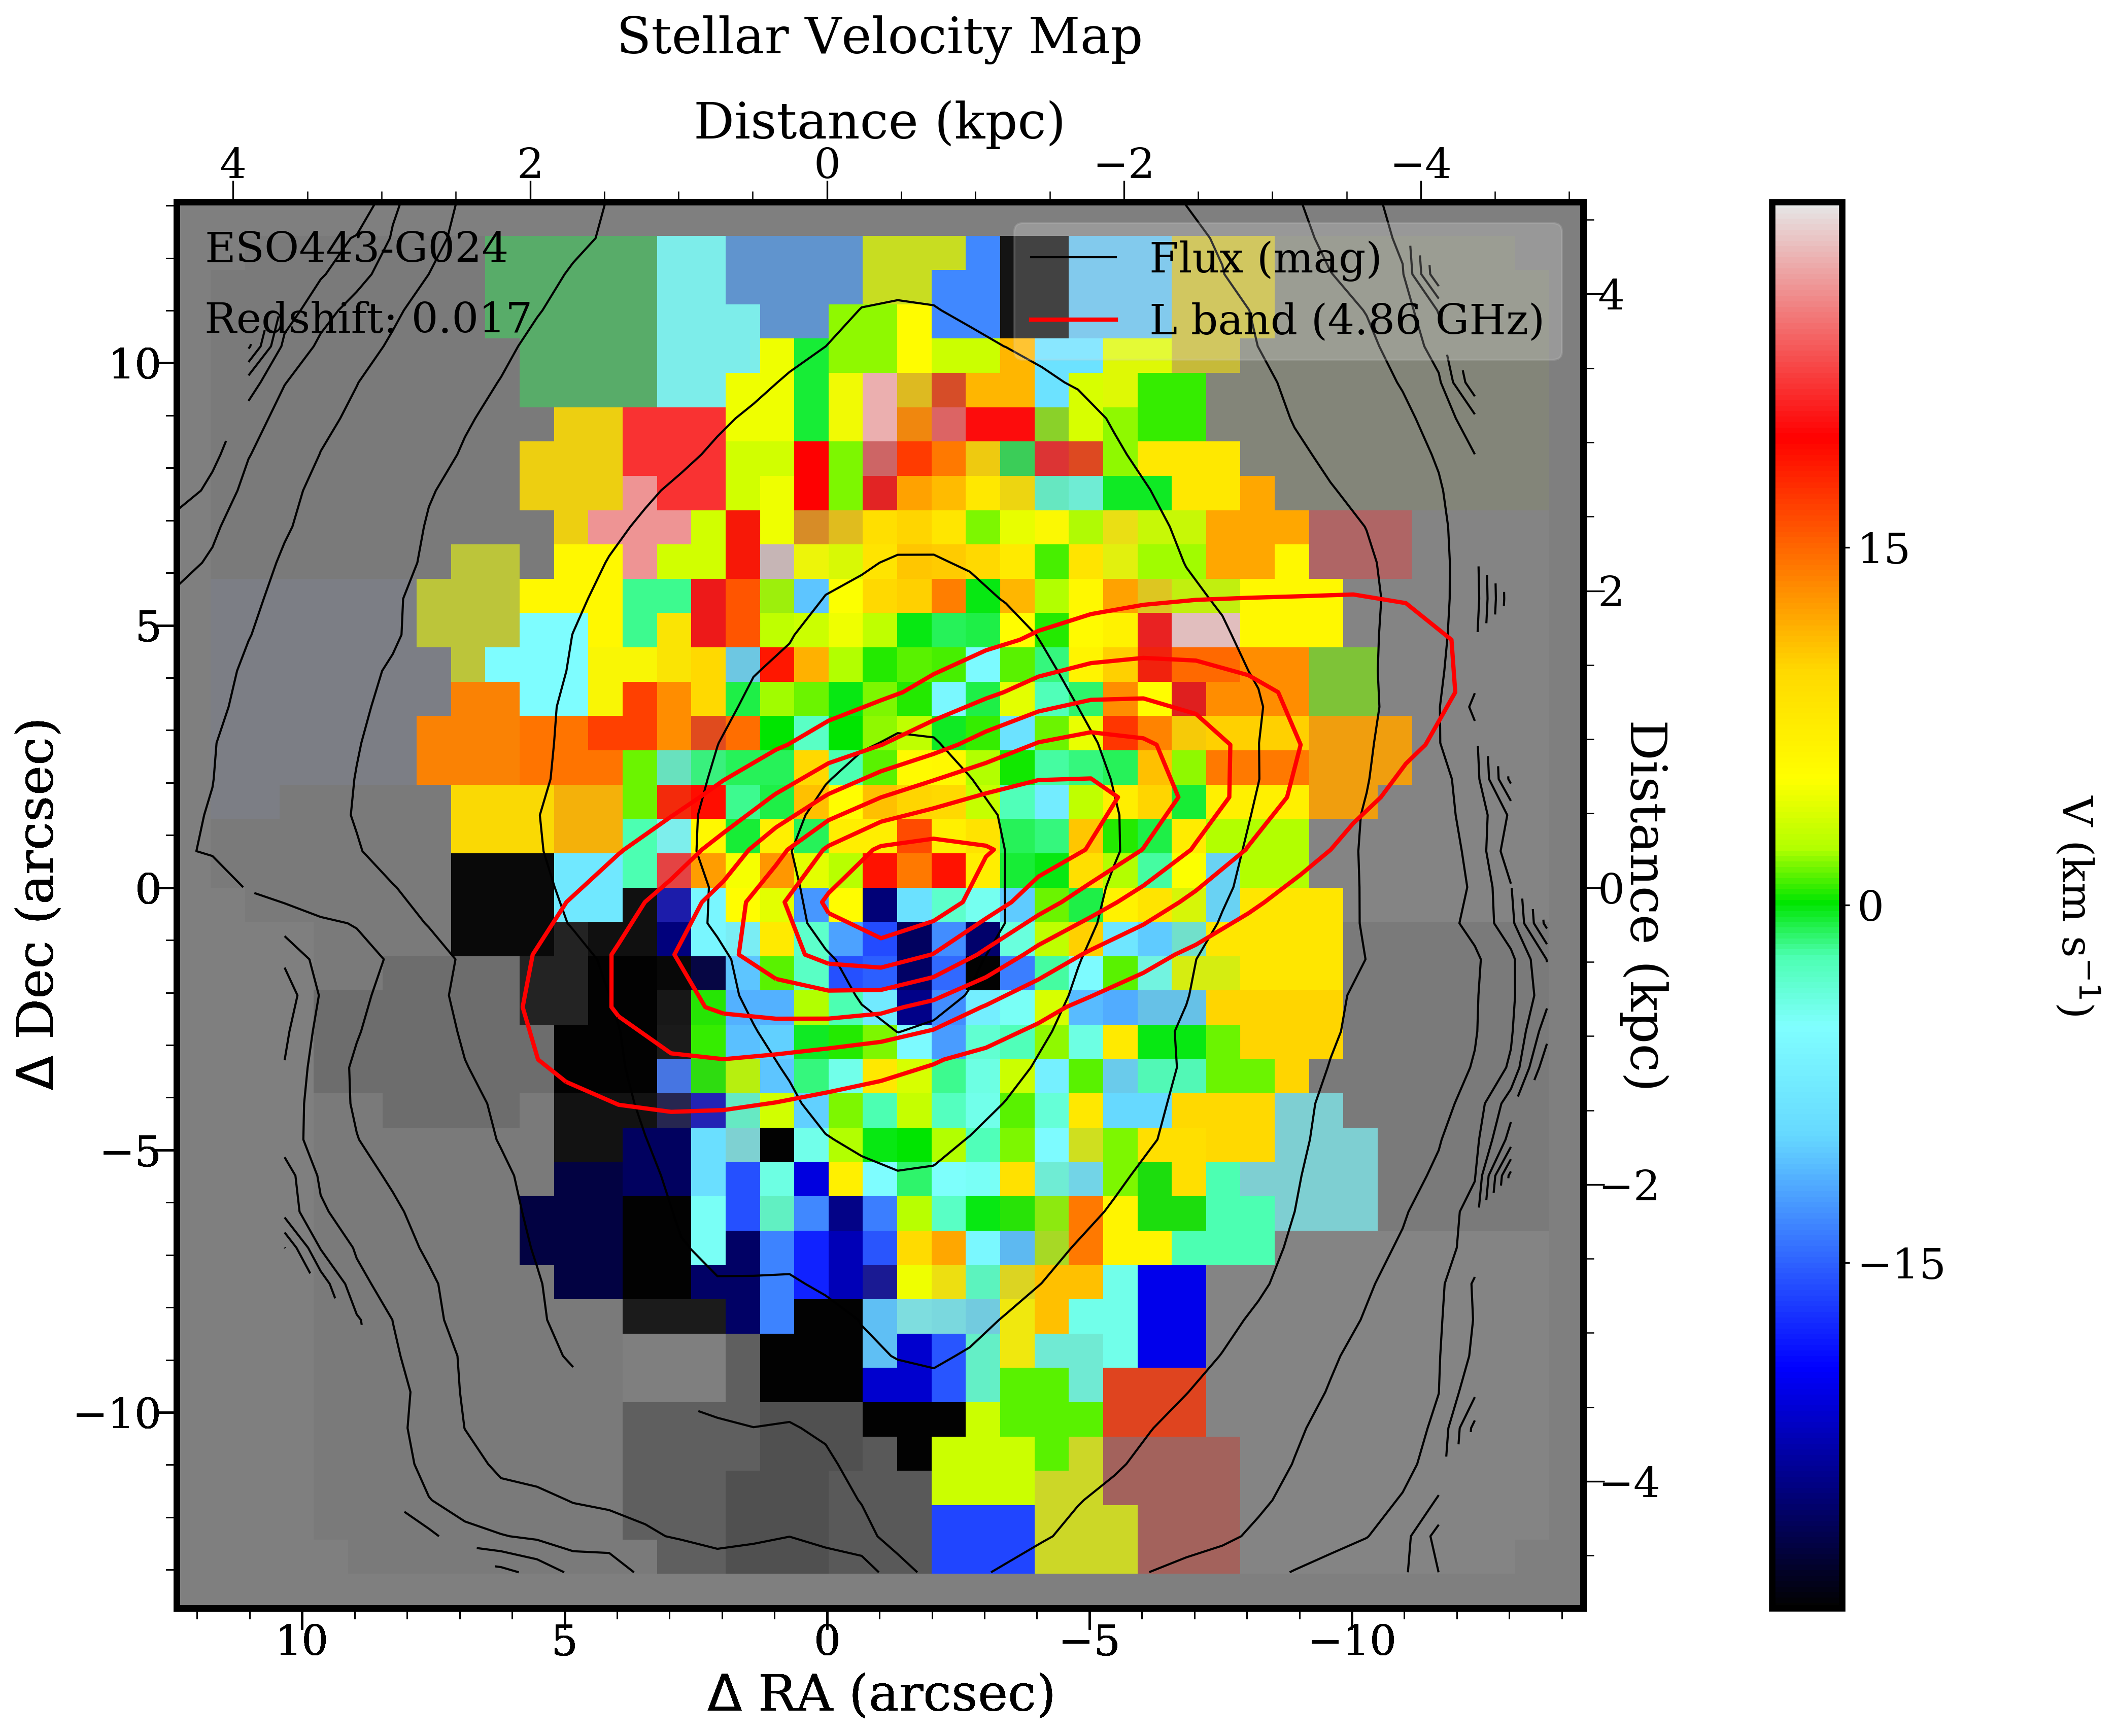
\includegraphics[width=0.245\textwidth]{Vmaps/eso443-g024_stellar_vel.png}
      \caption[VIMOS velocity maps]{Velocity for each galaxy in the VIMOS sample. Plots are ordered and contour colors are as in figure \ref{fig:Vstellar_img}}
      \label{fig:Vstellar_vel}
\end{figure*}

\begin{figure*}
      \centering
      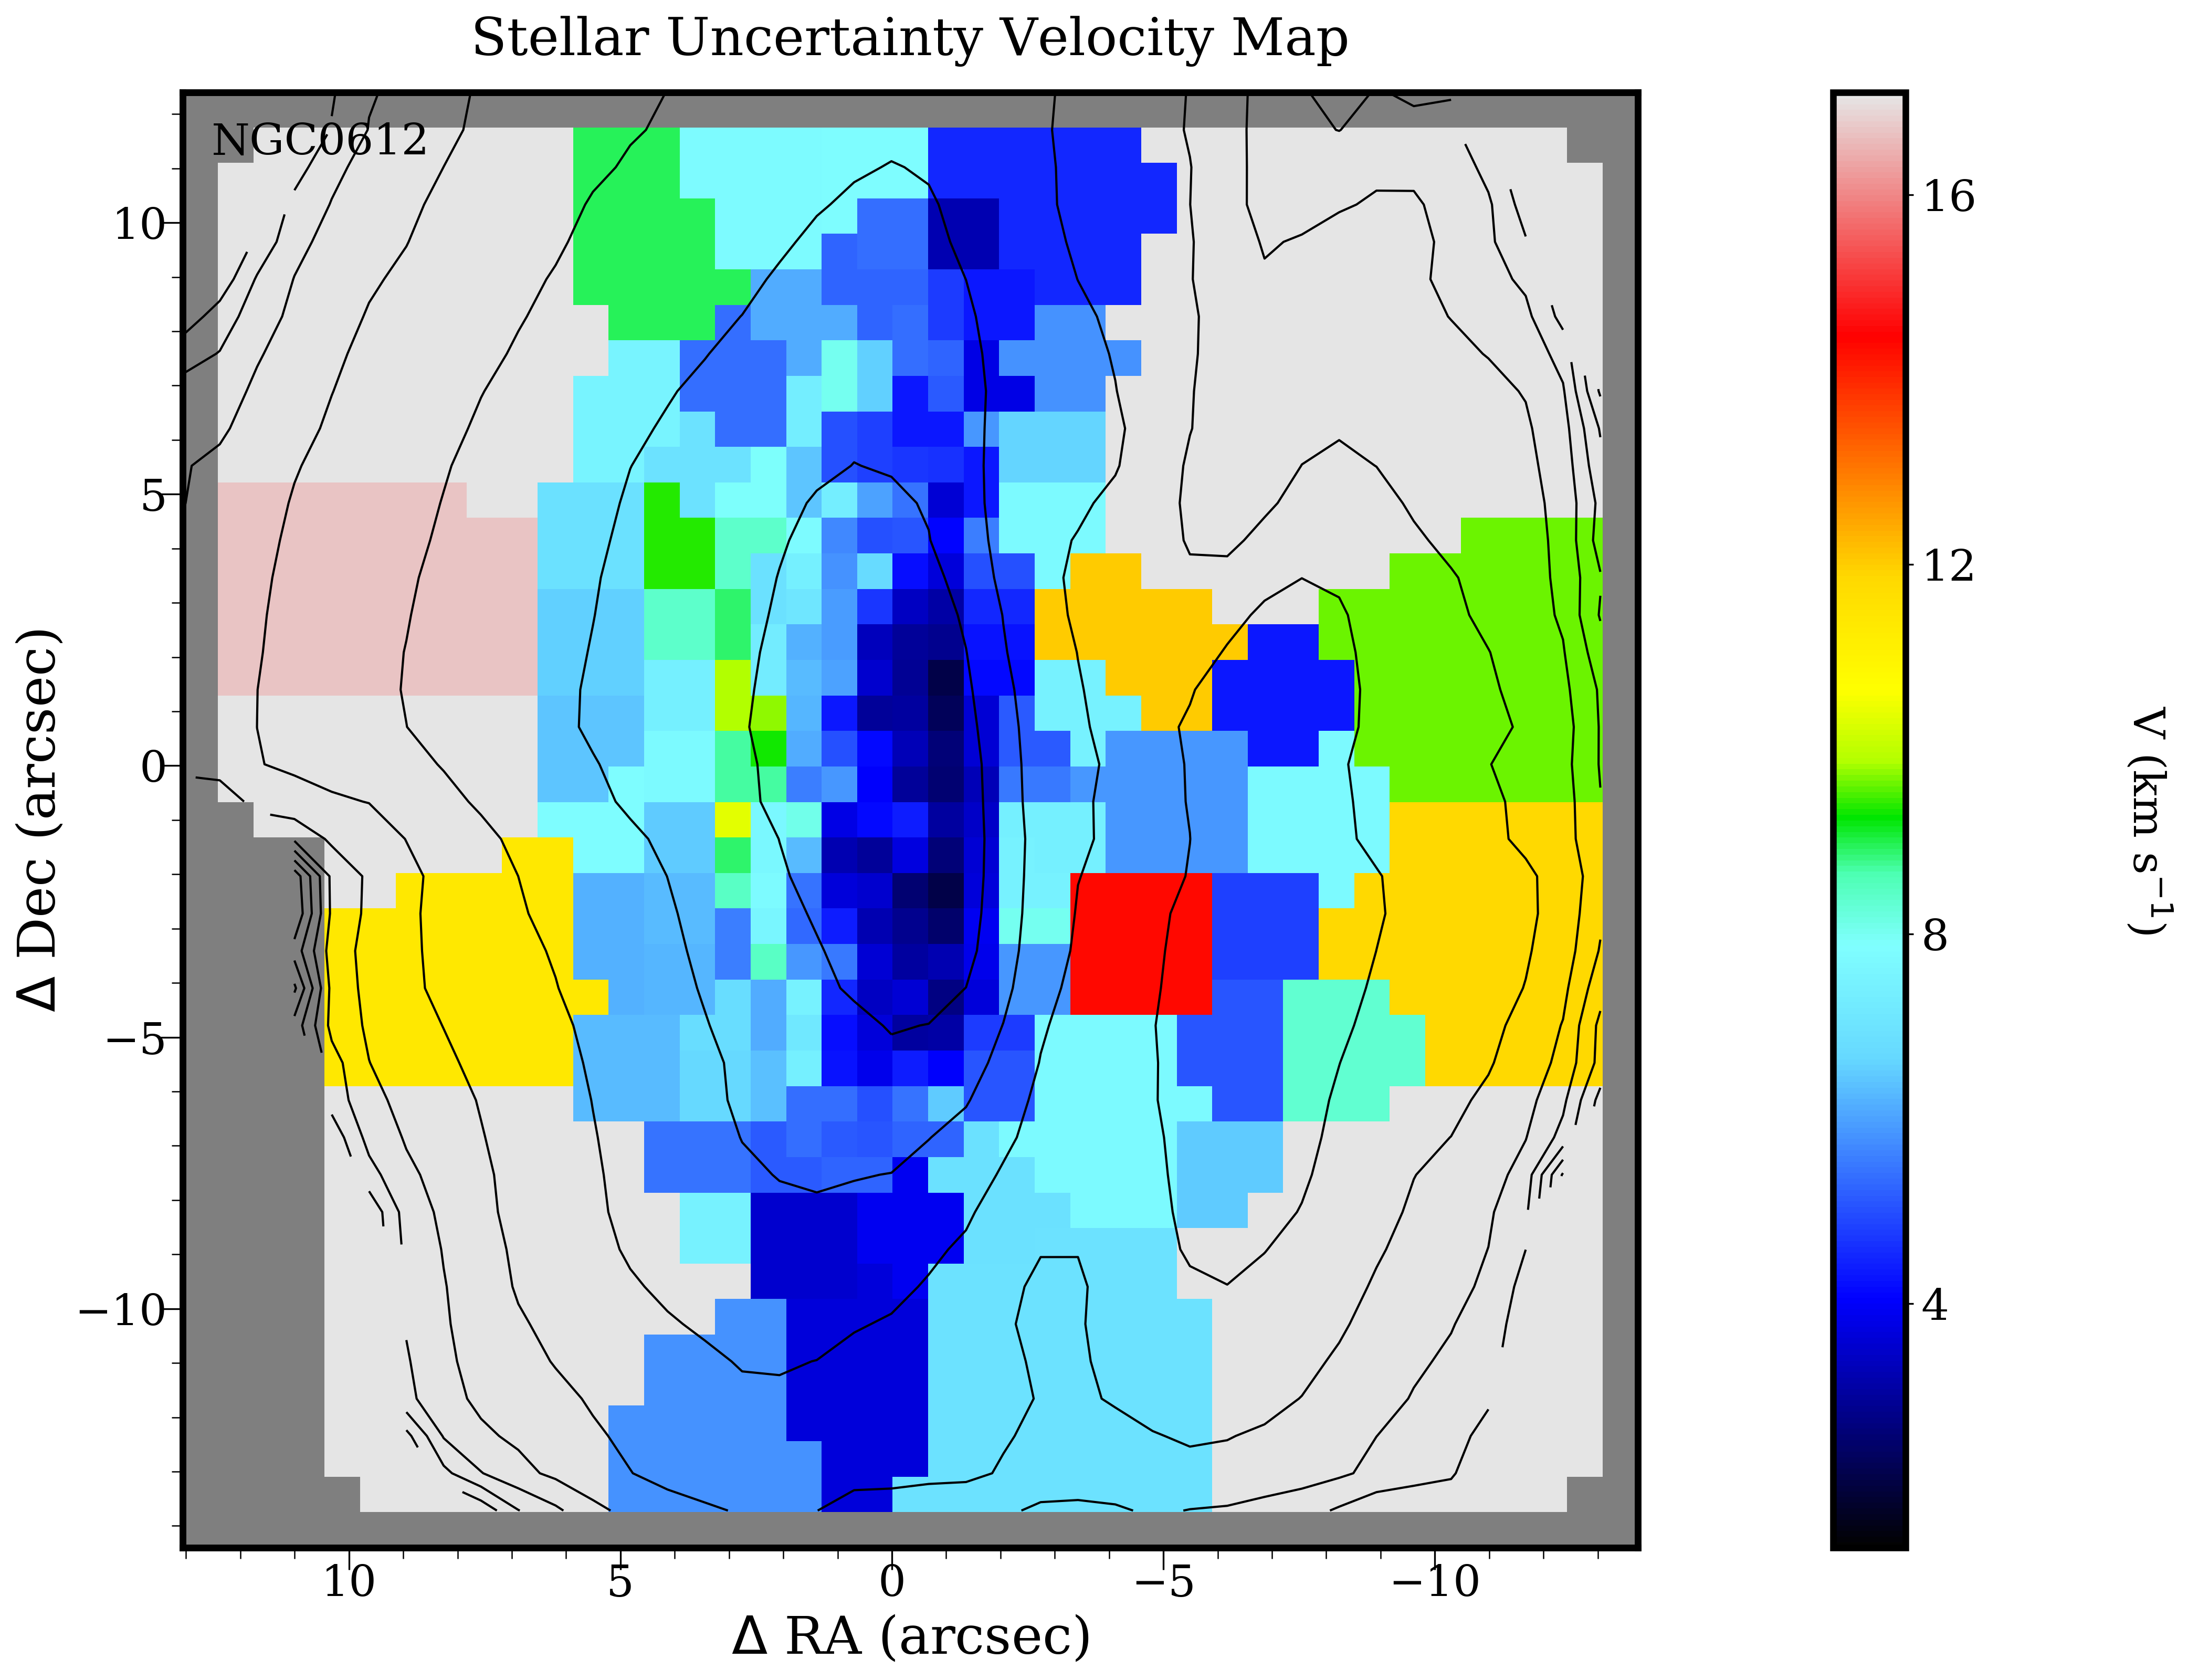
\includegraphics[width=0.245\textwidth]{Vmaps/ngc0612_stellar_vel_uncert.png}
      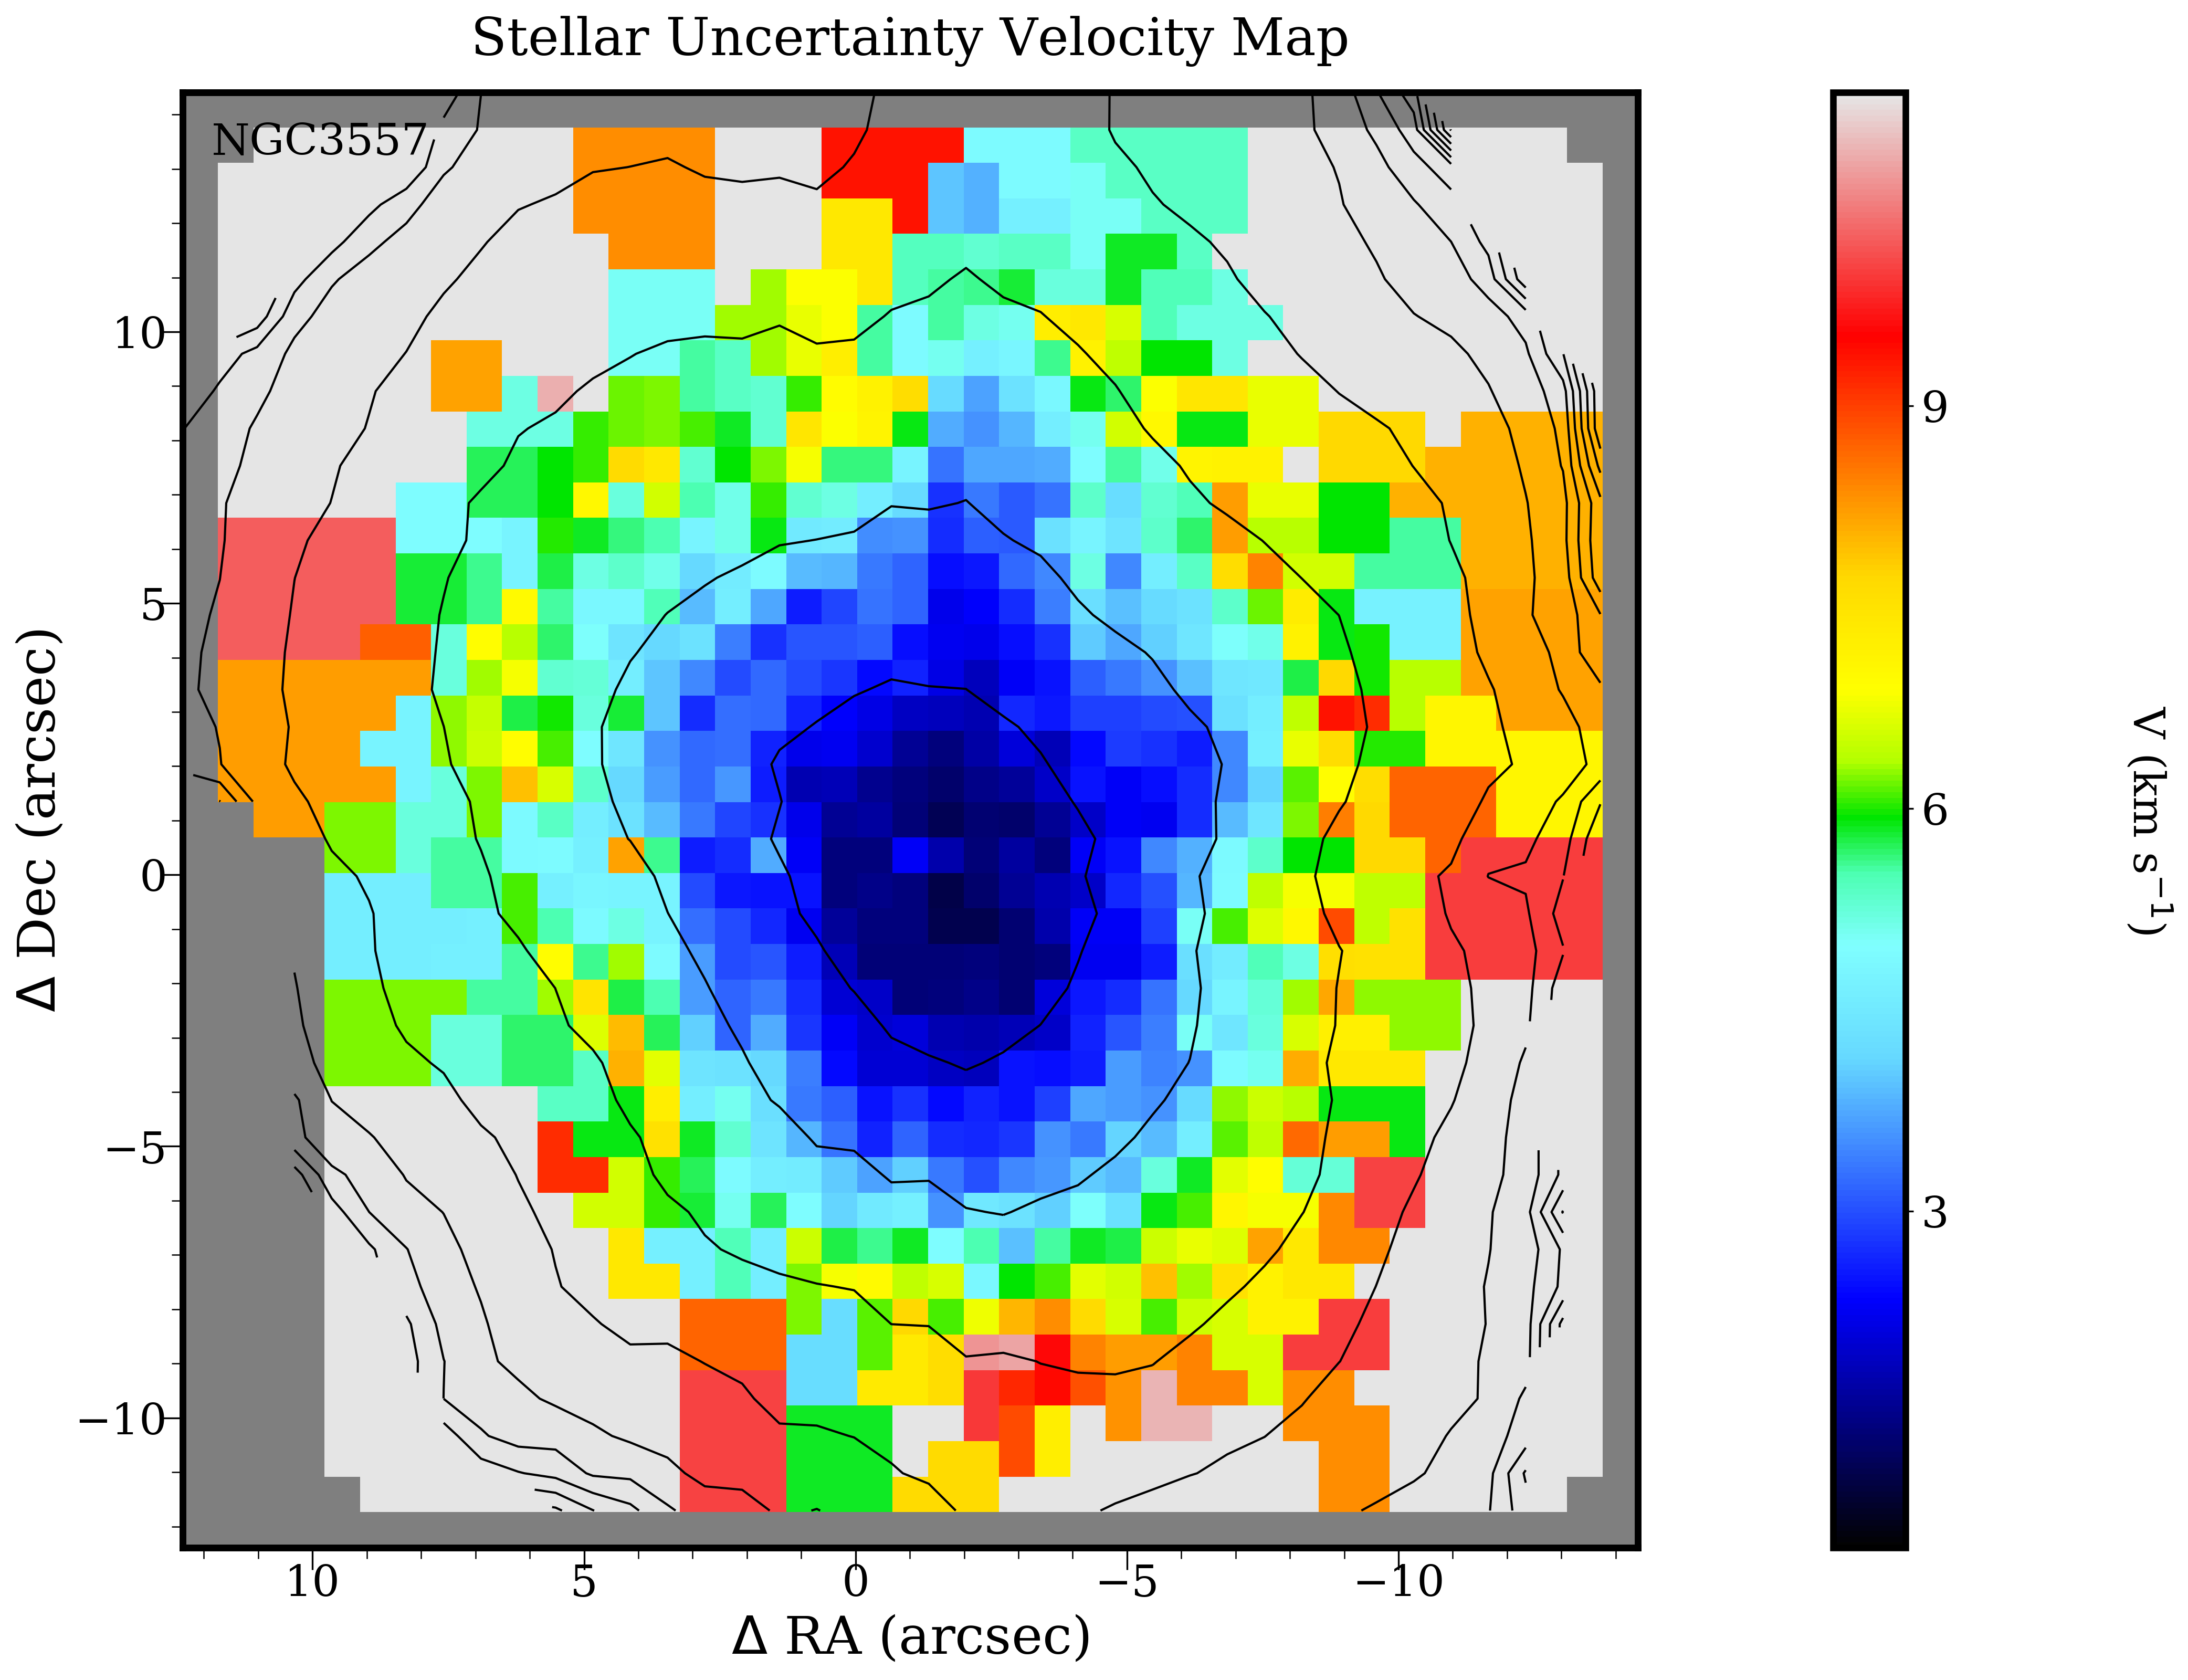
\includegraphics[width=0.245\textwidth]{Vmaps/ngc3557_stellar_vel_uncert.png}
      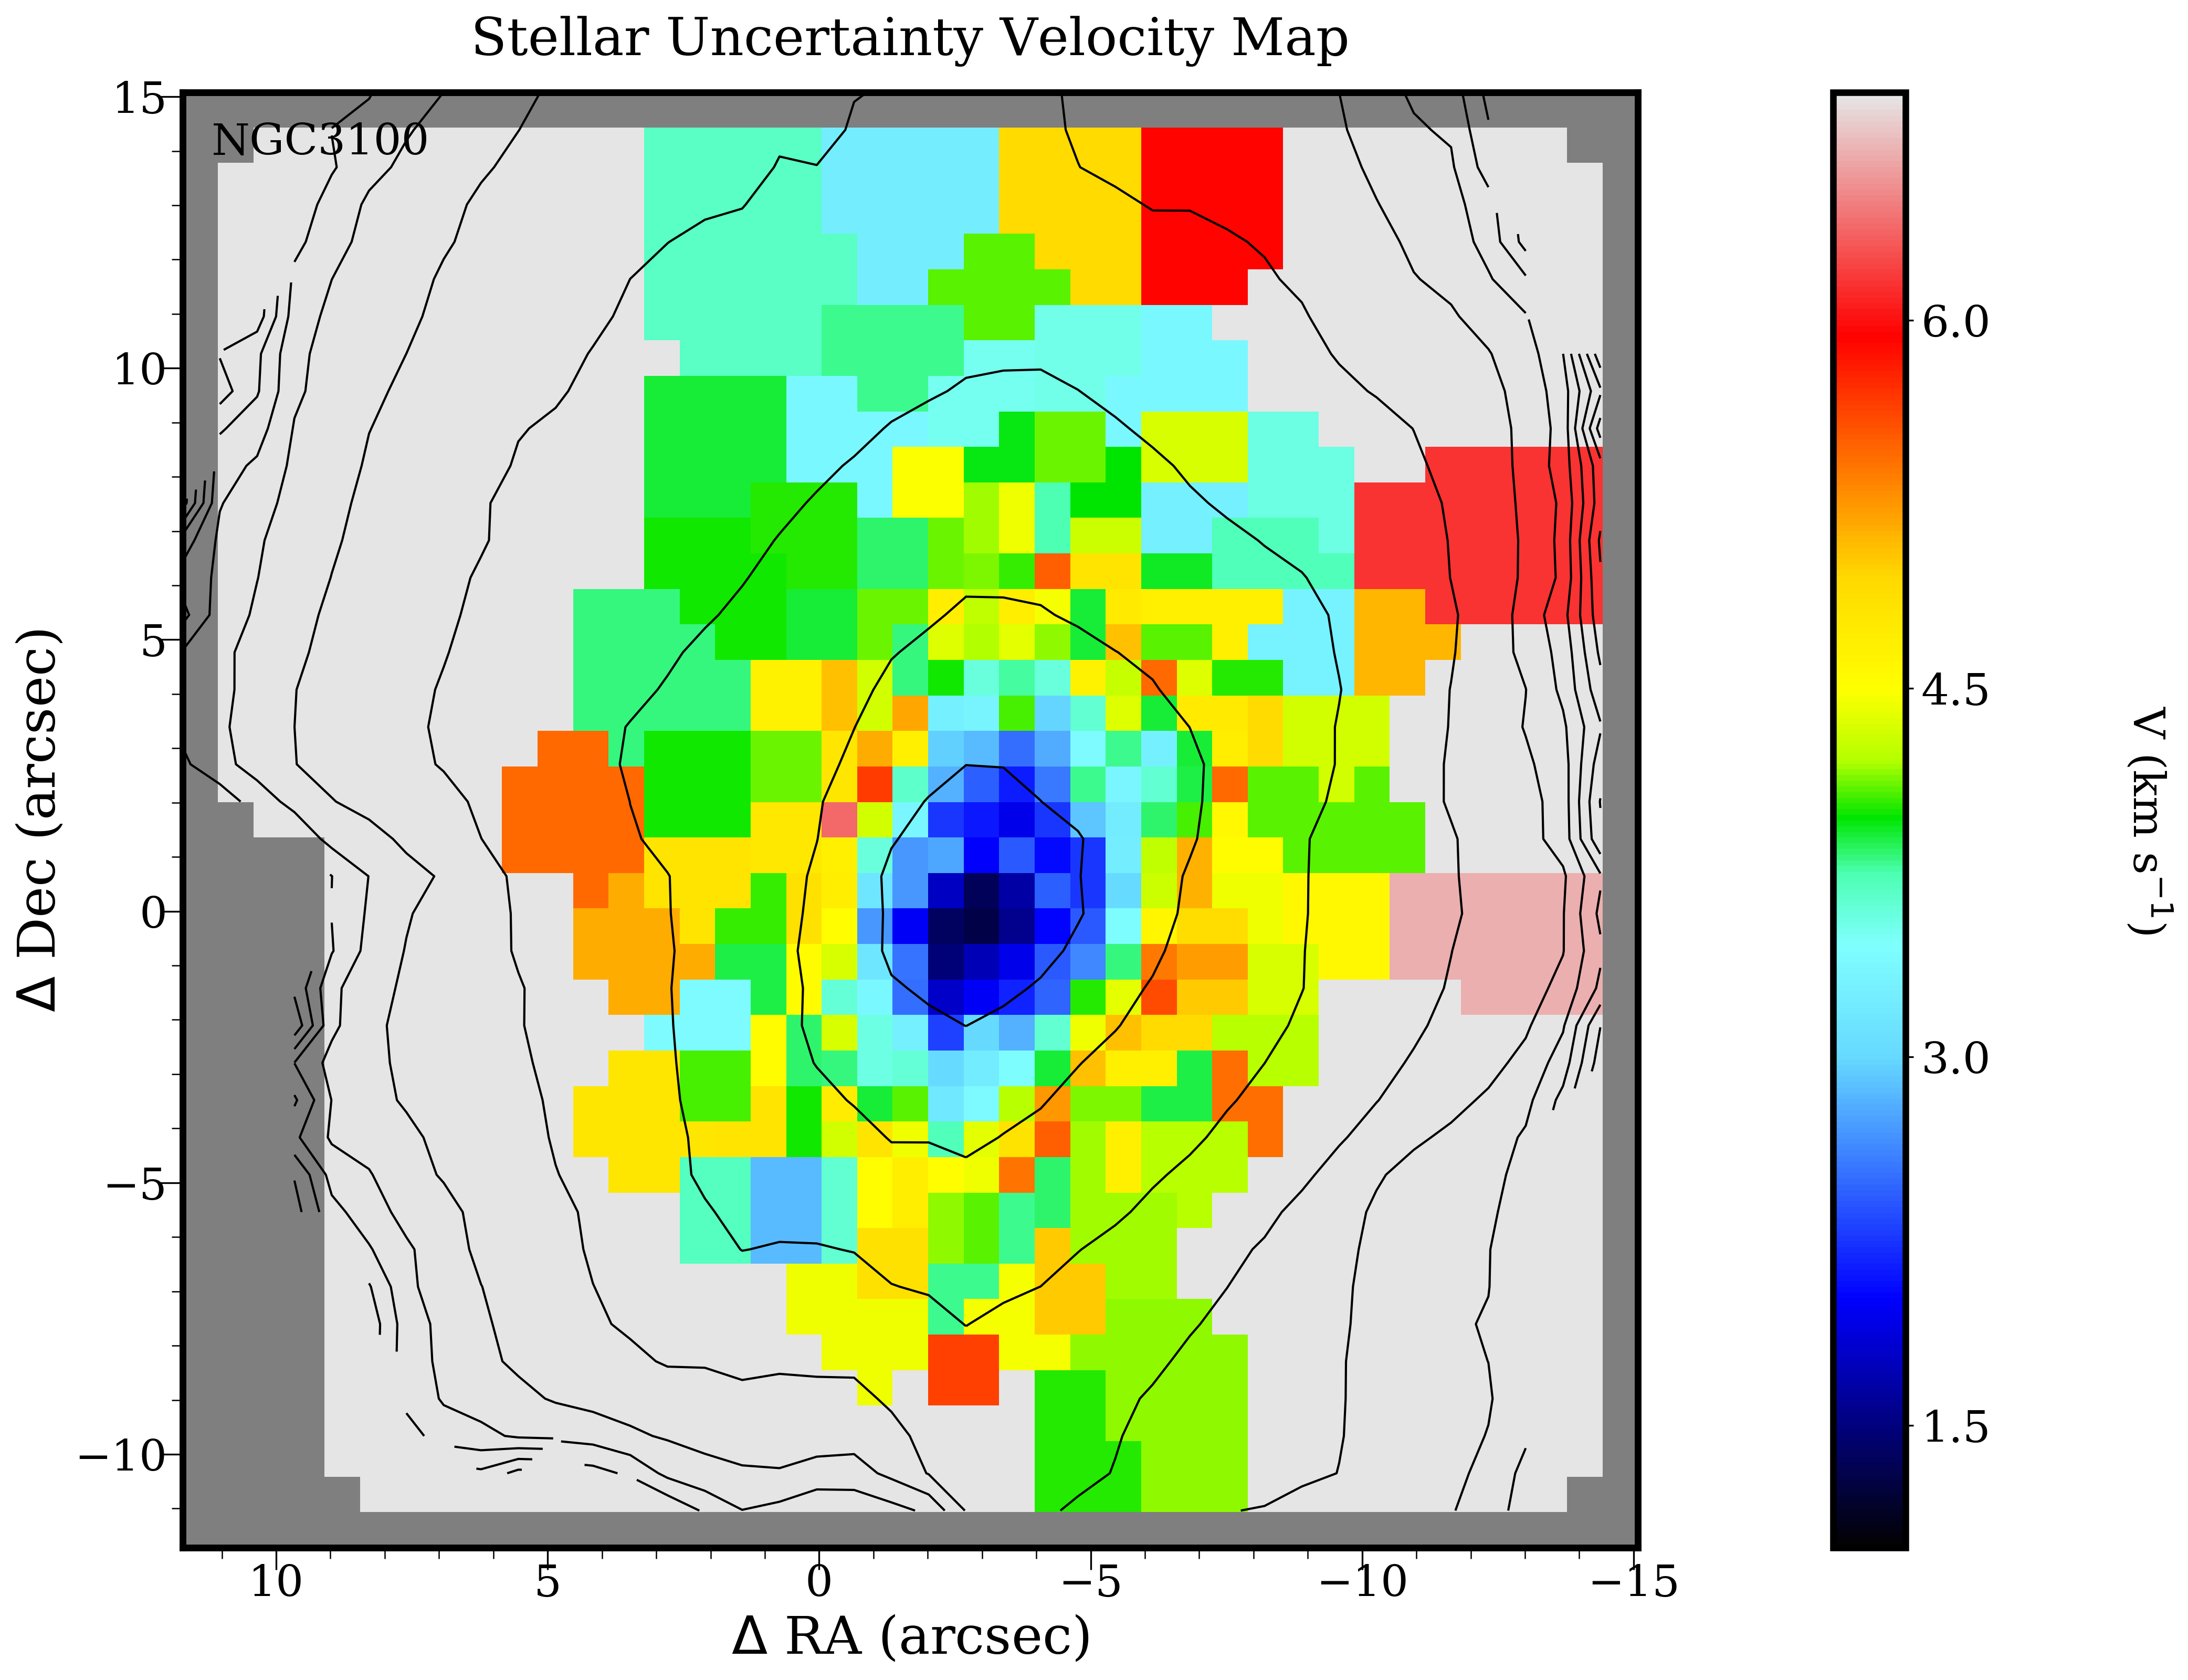
\includegraphics[width=0.245\textwidth]{Vmaps/ngc3100_stellar_vel_uncert.png}
      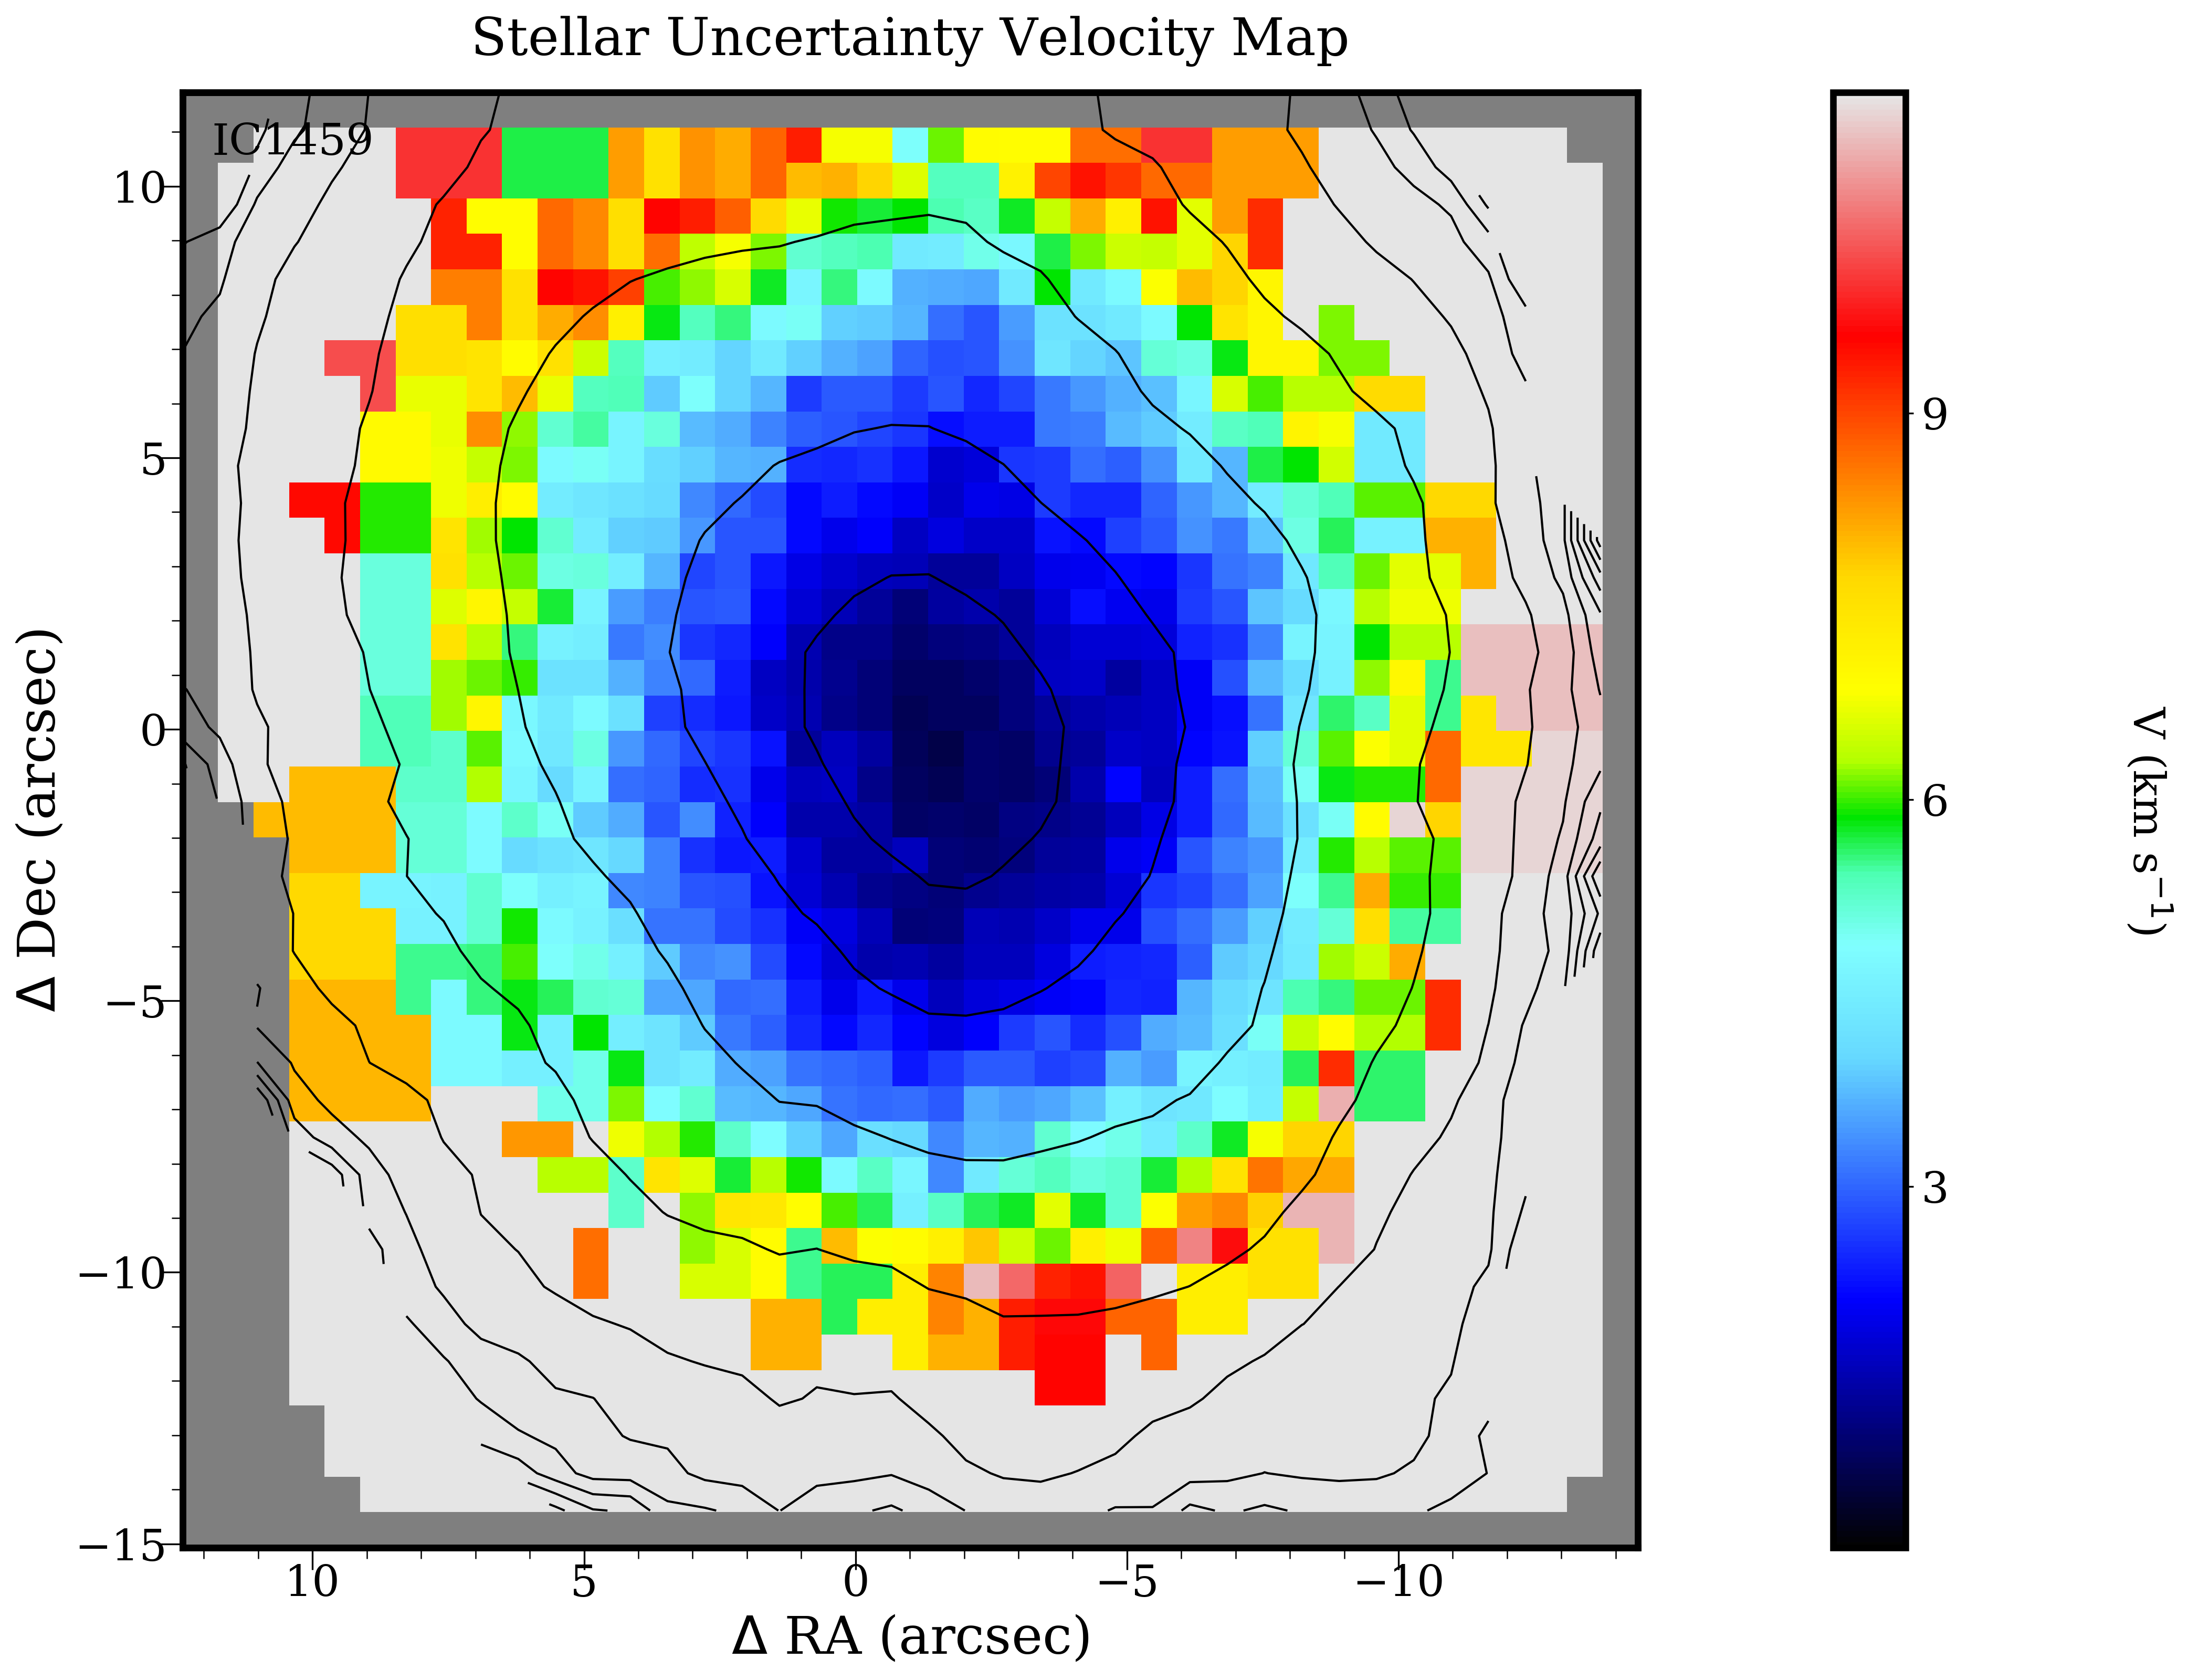
\includegraphics[width=0.245\textwidth]{Vmaps/ic1459_stellar_vel_uncert.png}
      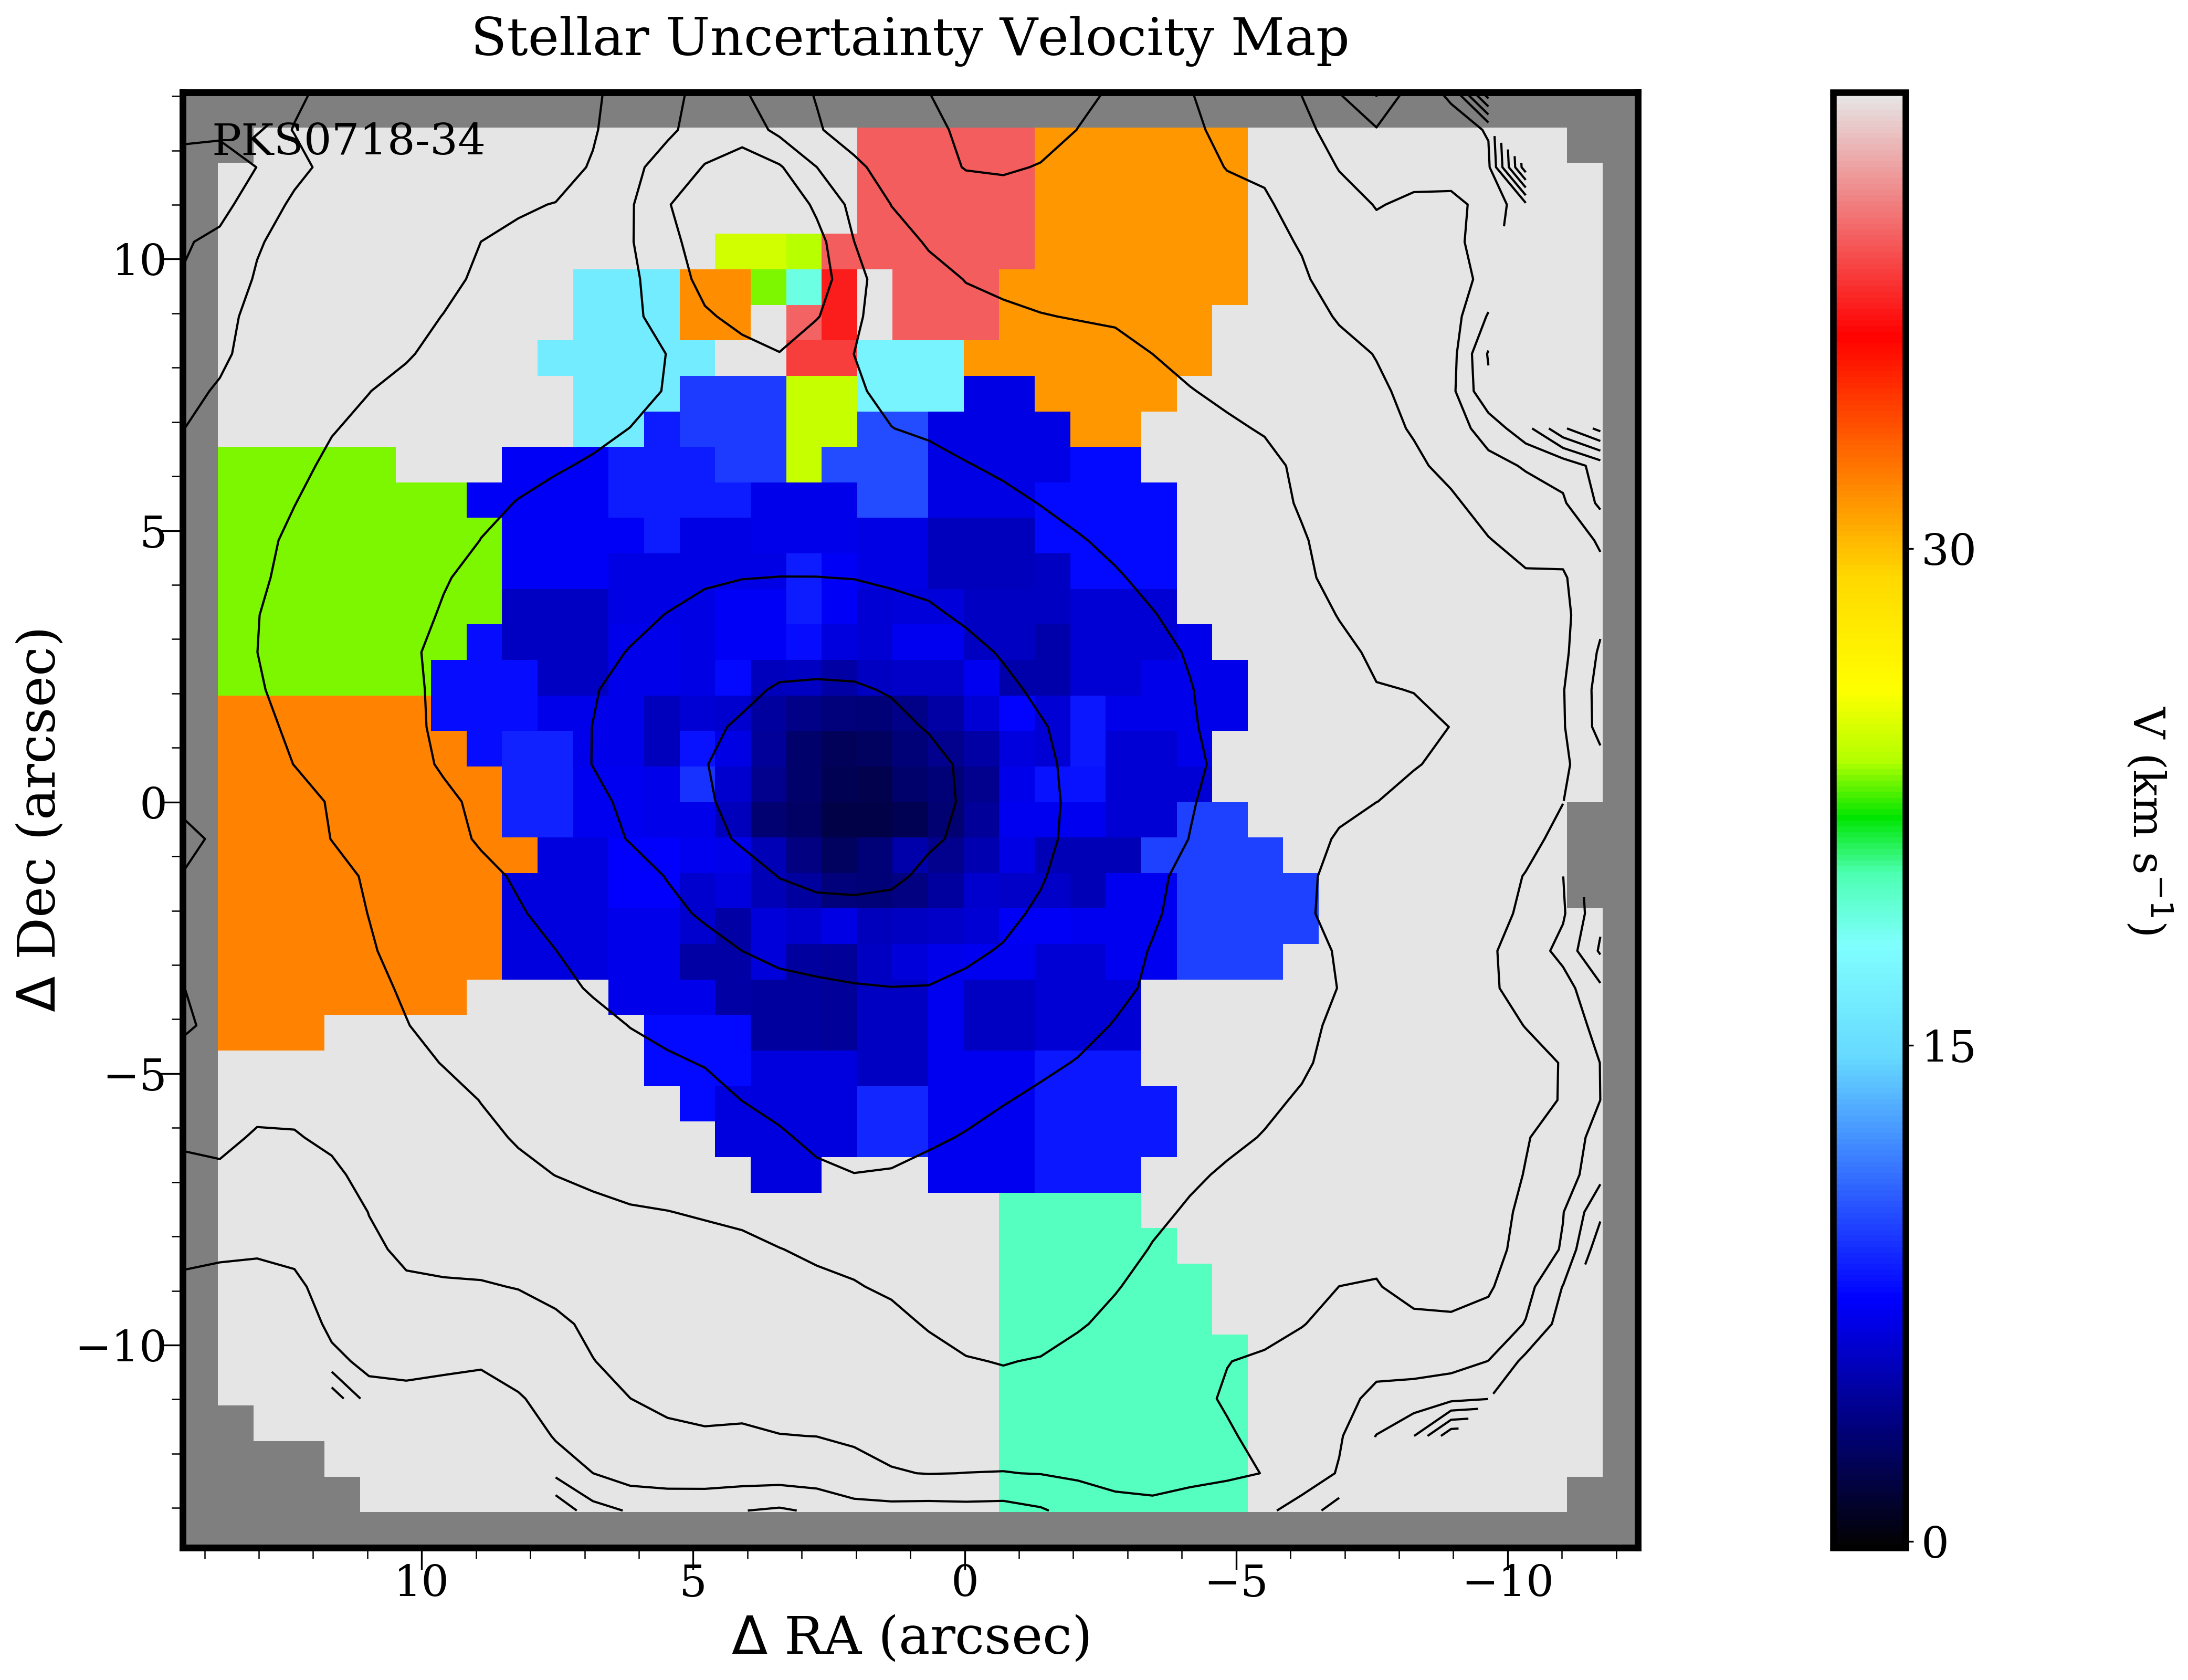
\includegraphics[width=0.245\textwidth]{Vmaps/pks0718-34_stellar_vel_uncert.png}
      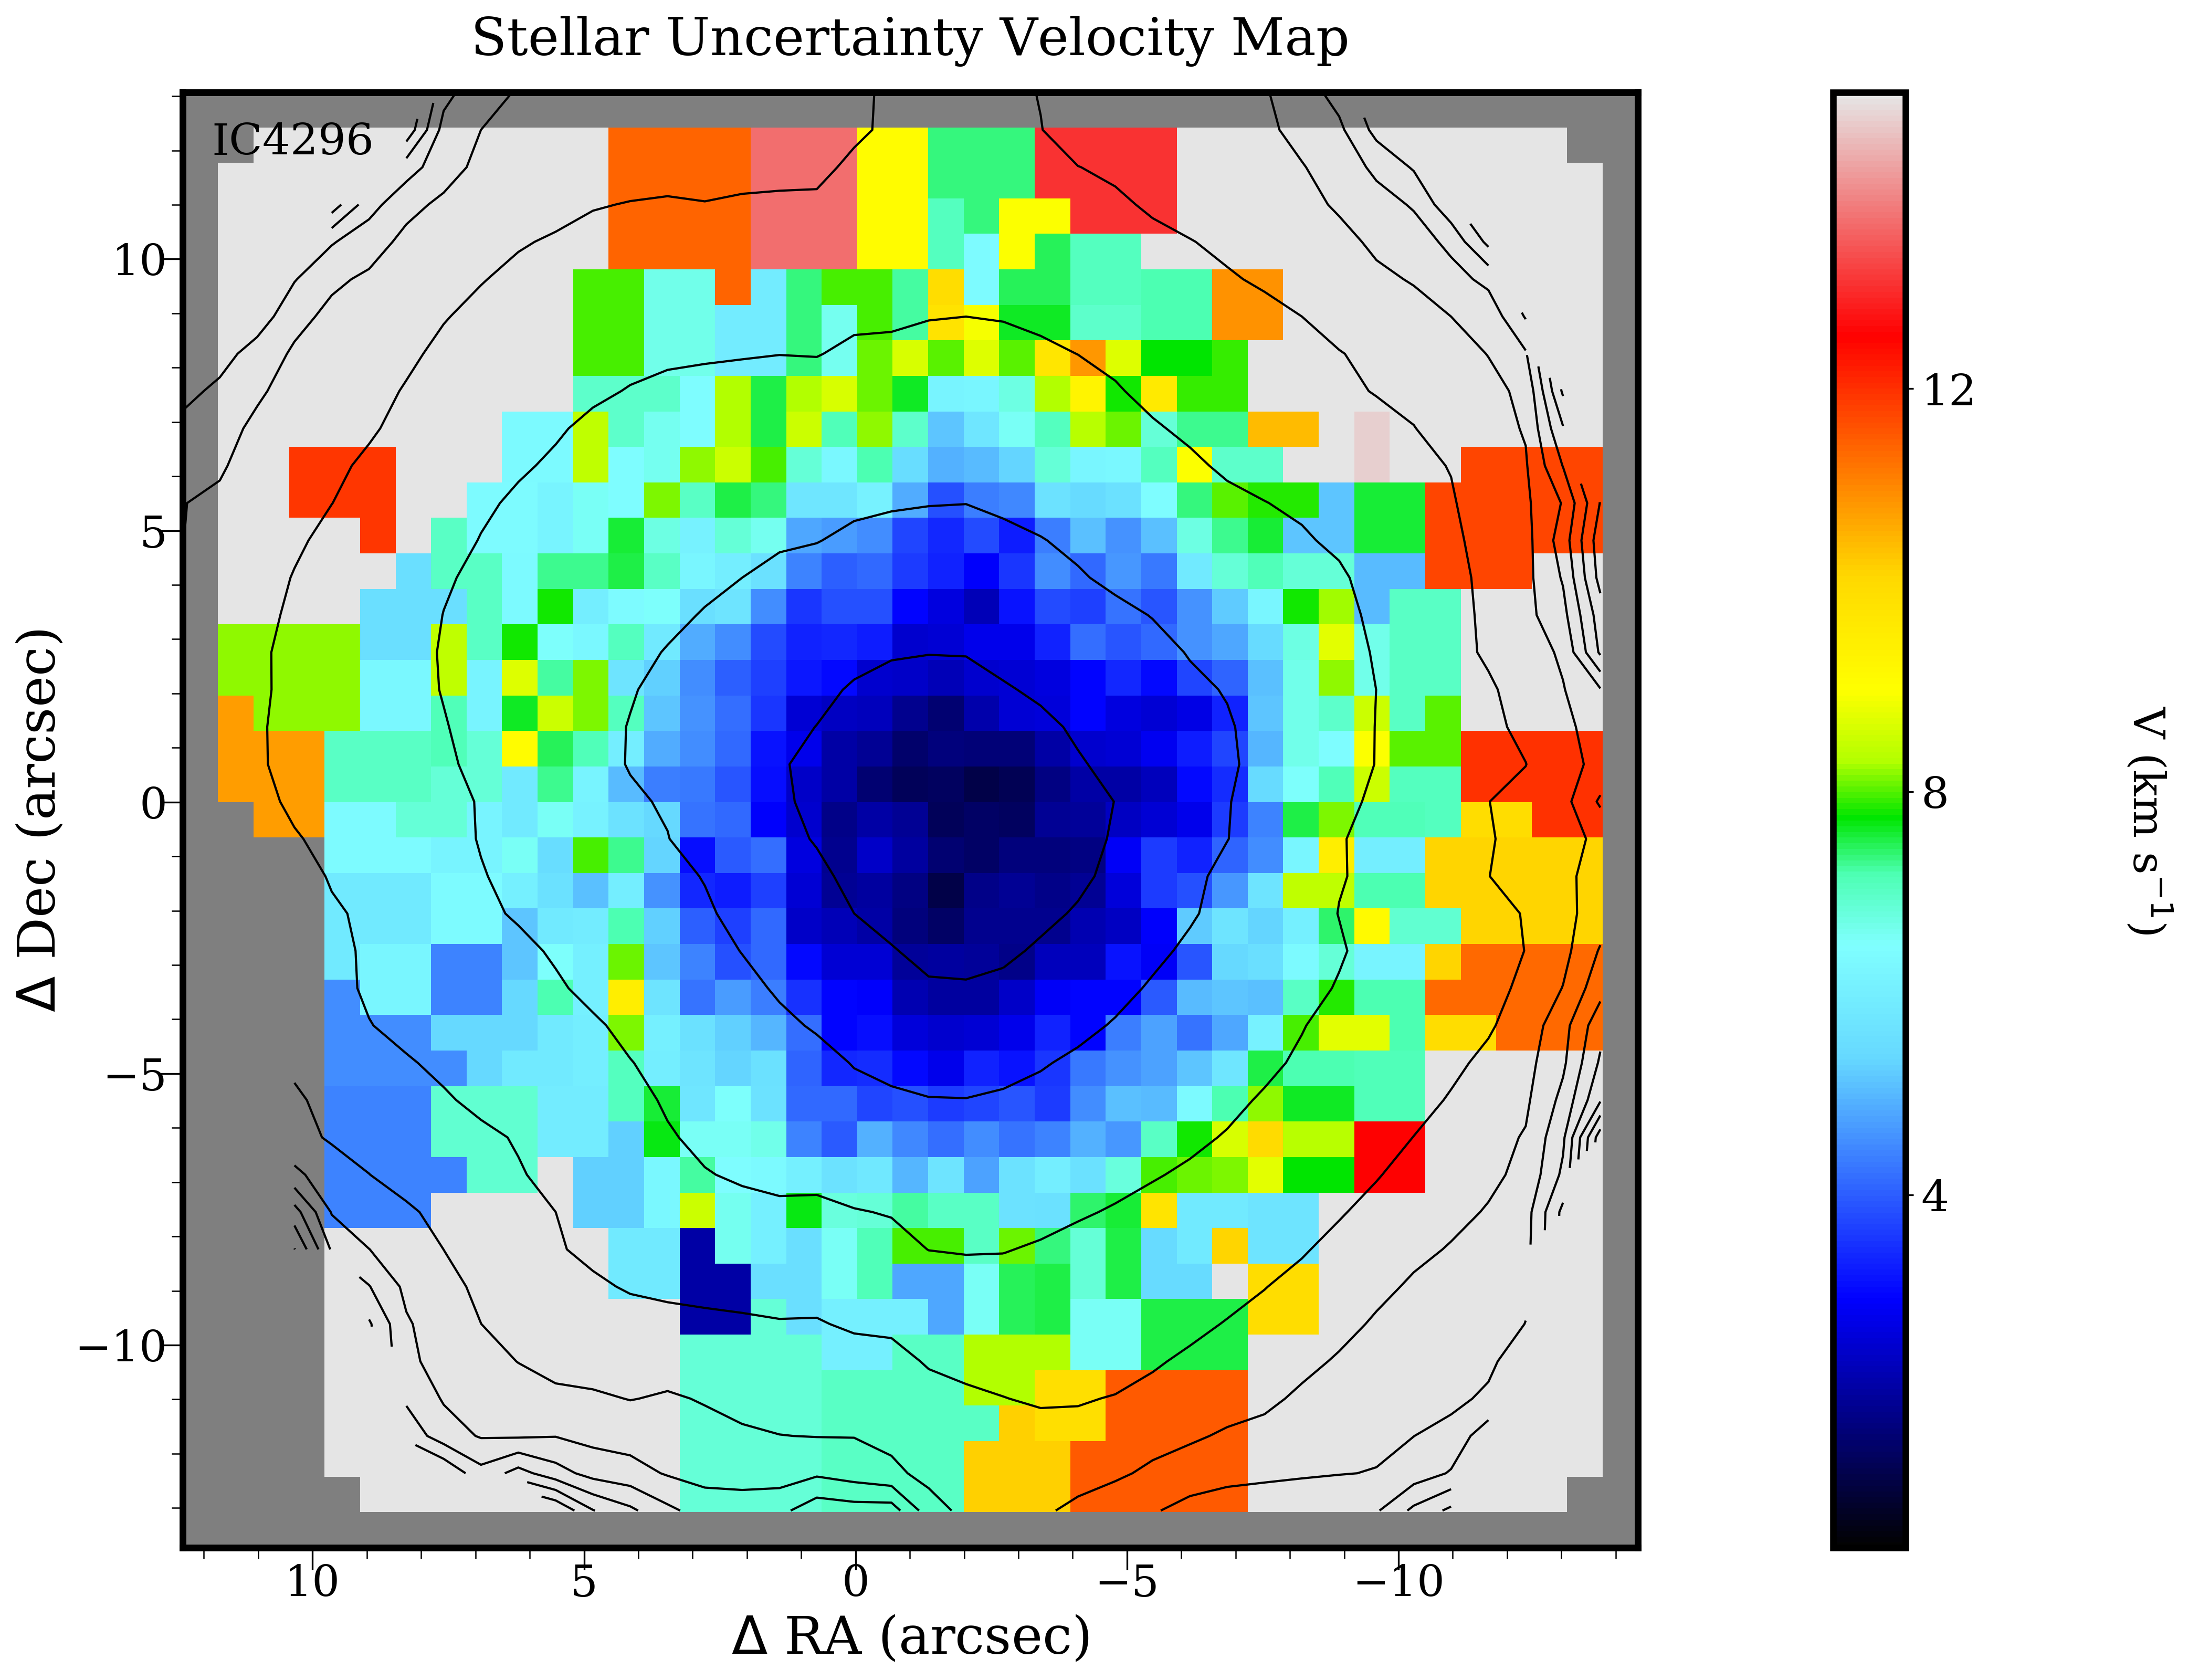
\includegraphics[width=0.245\textwidth]{Vmaps/ic4296_stellar_vel_uncert.png}
      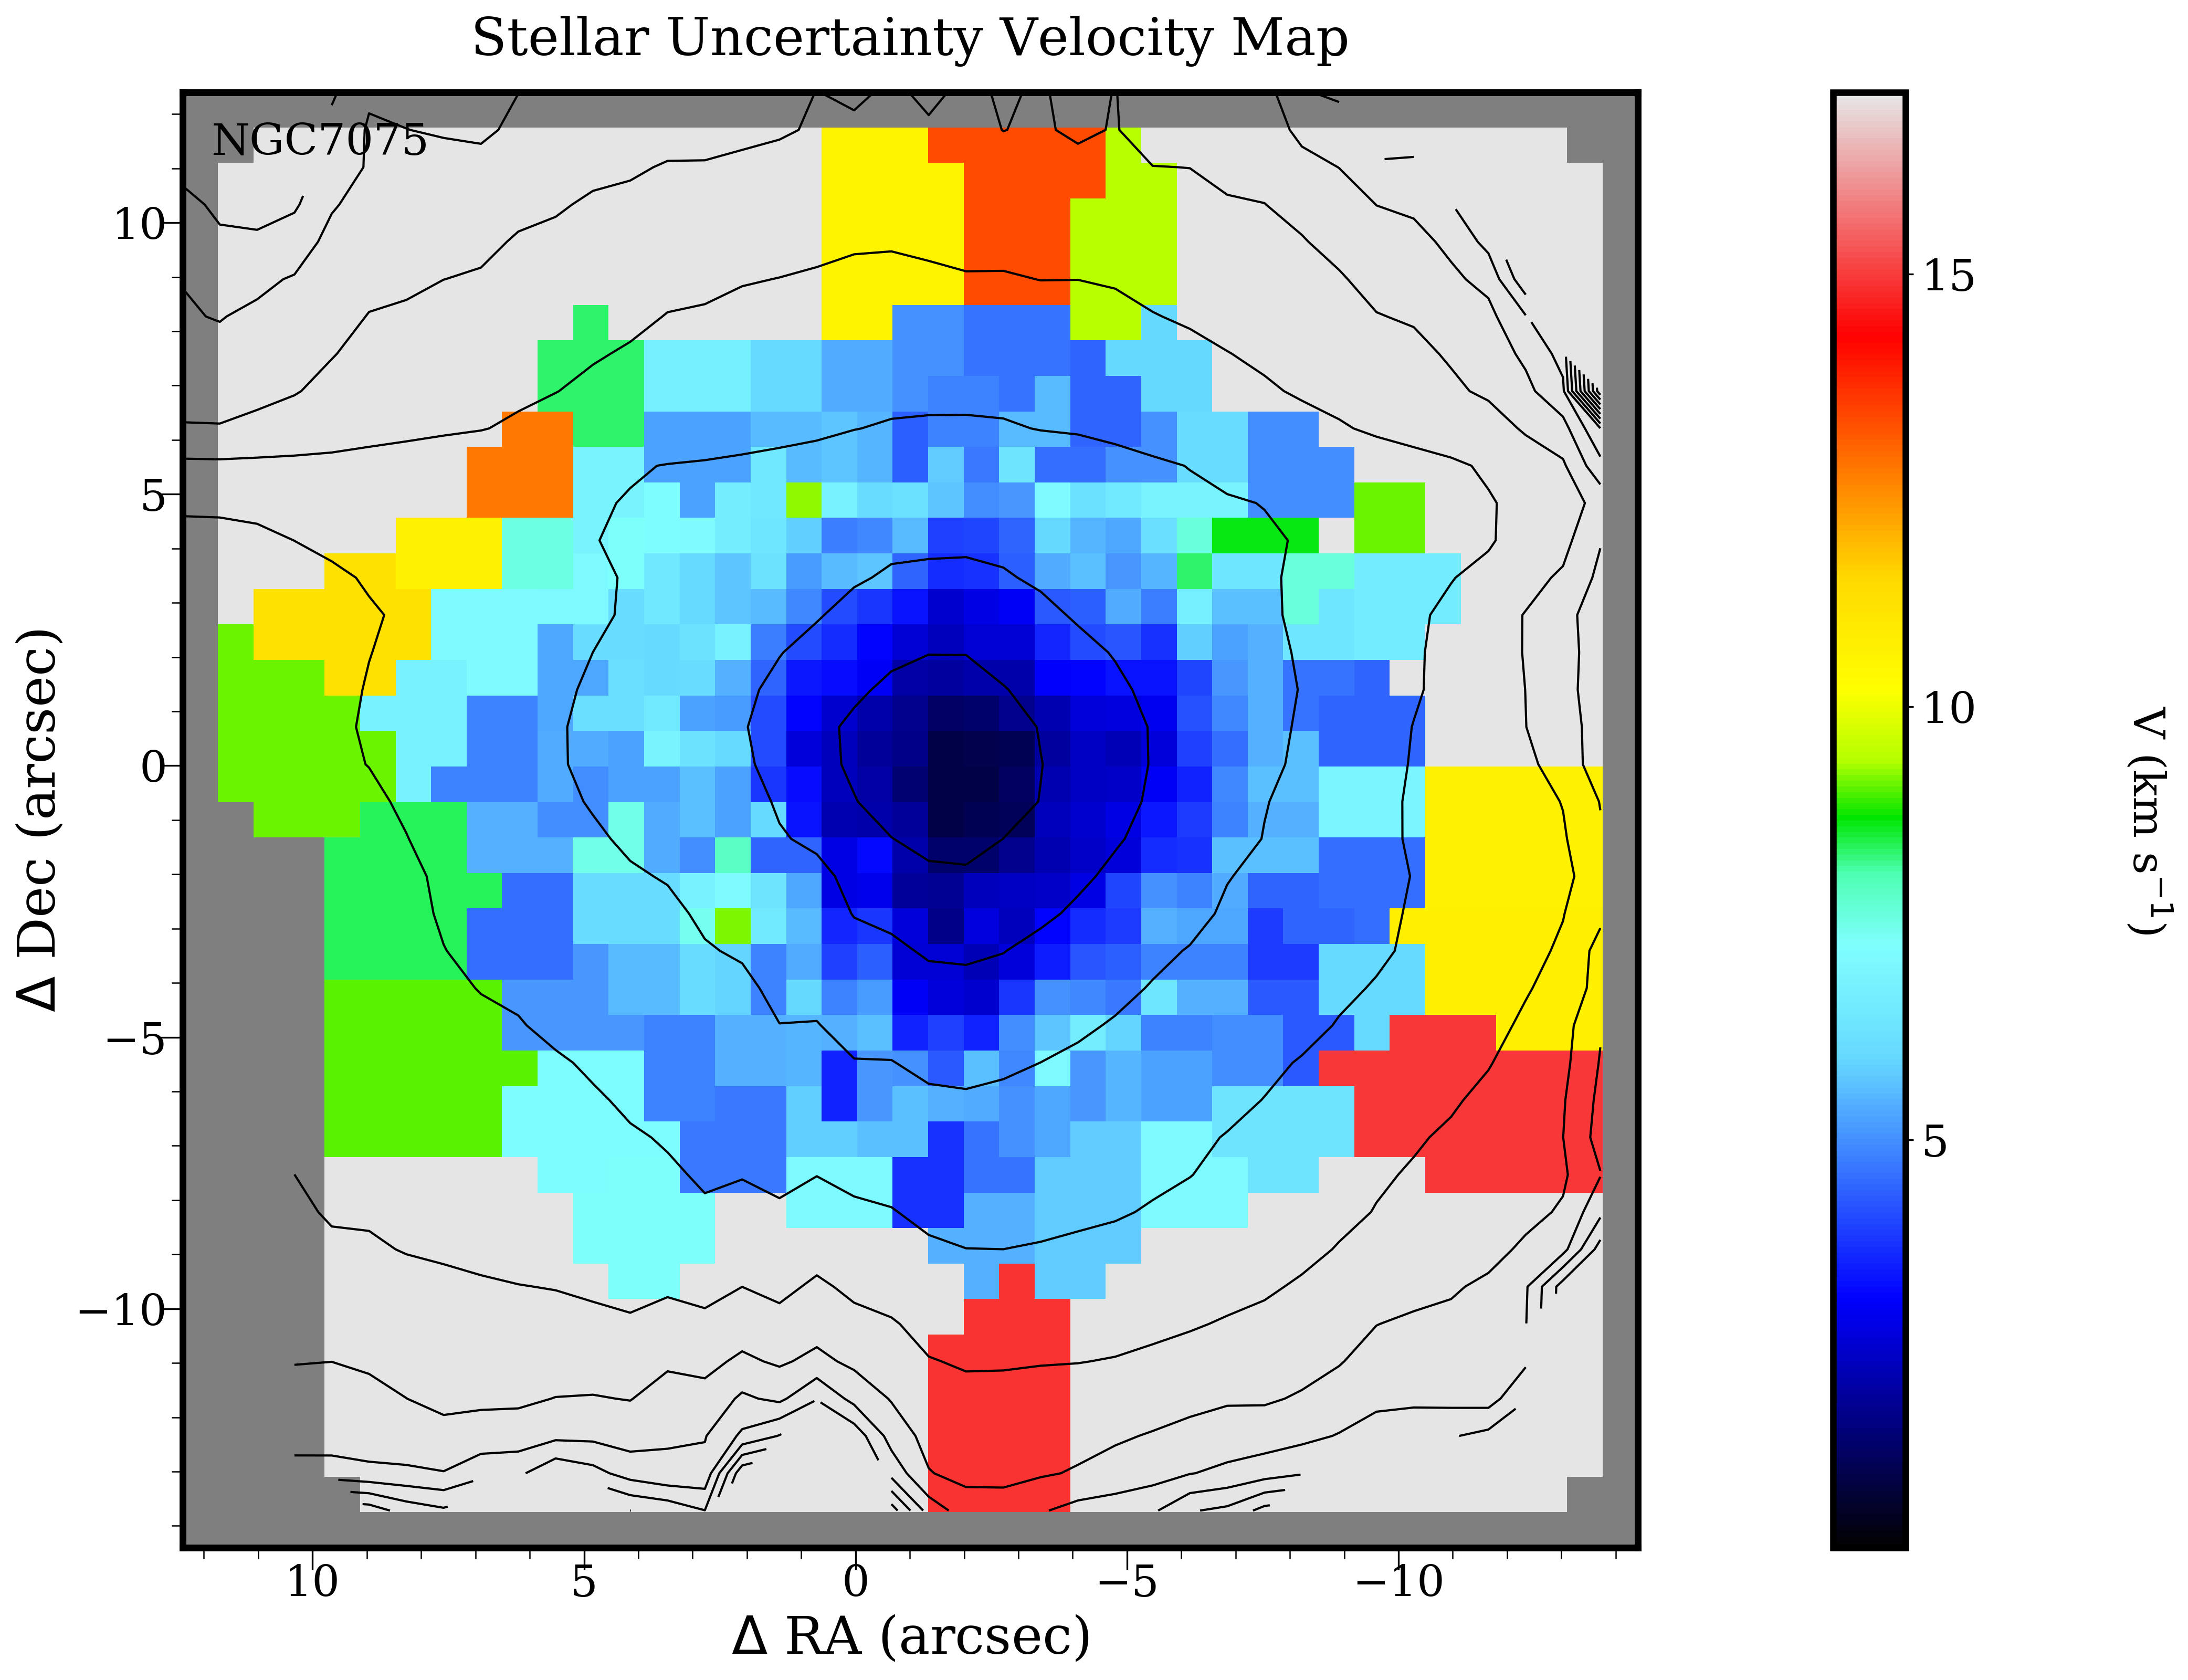
\includegraphics[width=0.245\textwidth]{Vmaps/ngc7075_stellar_vel_uncert.png}
      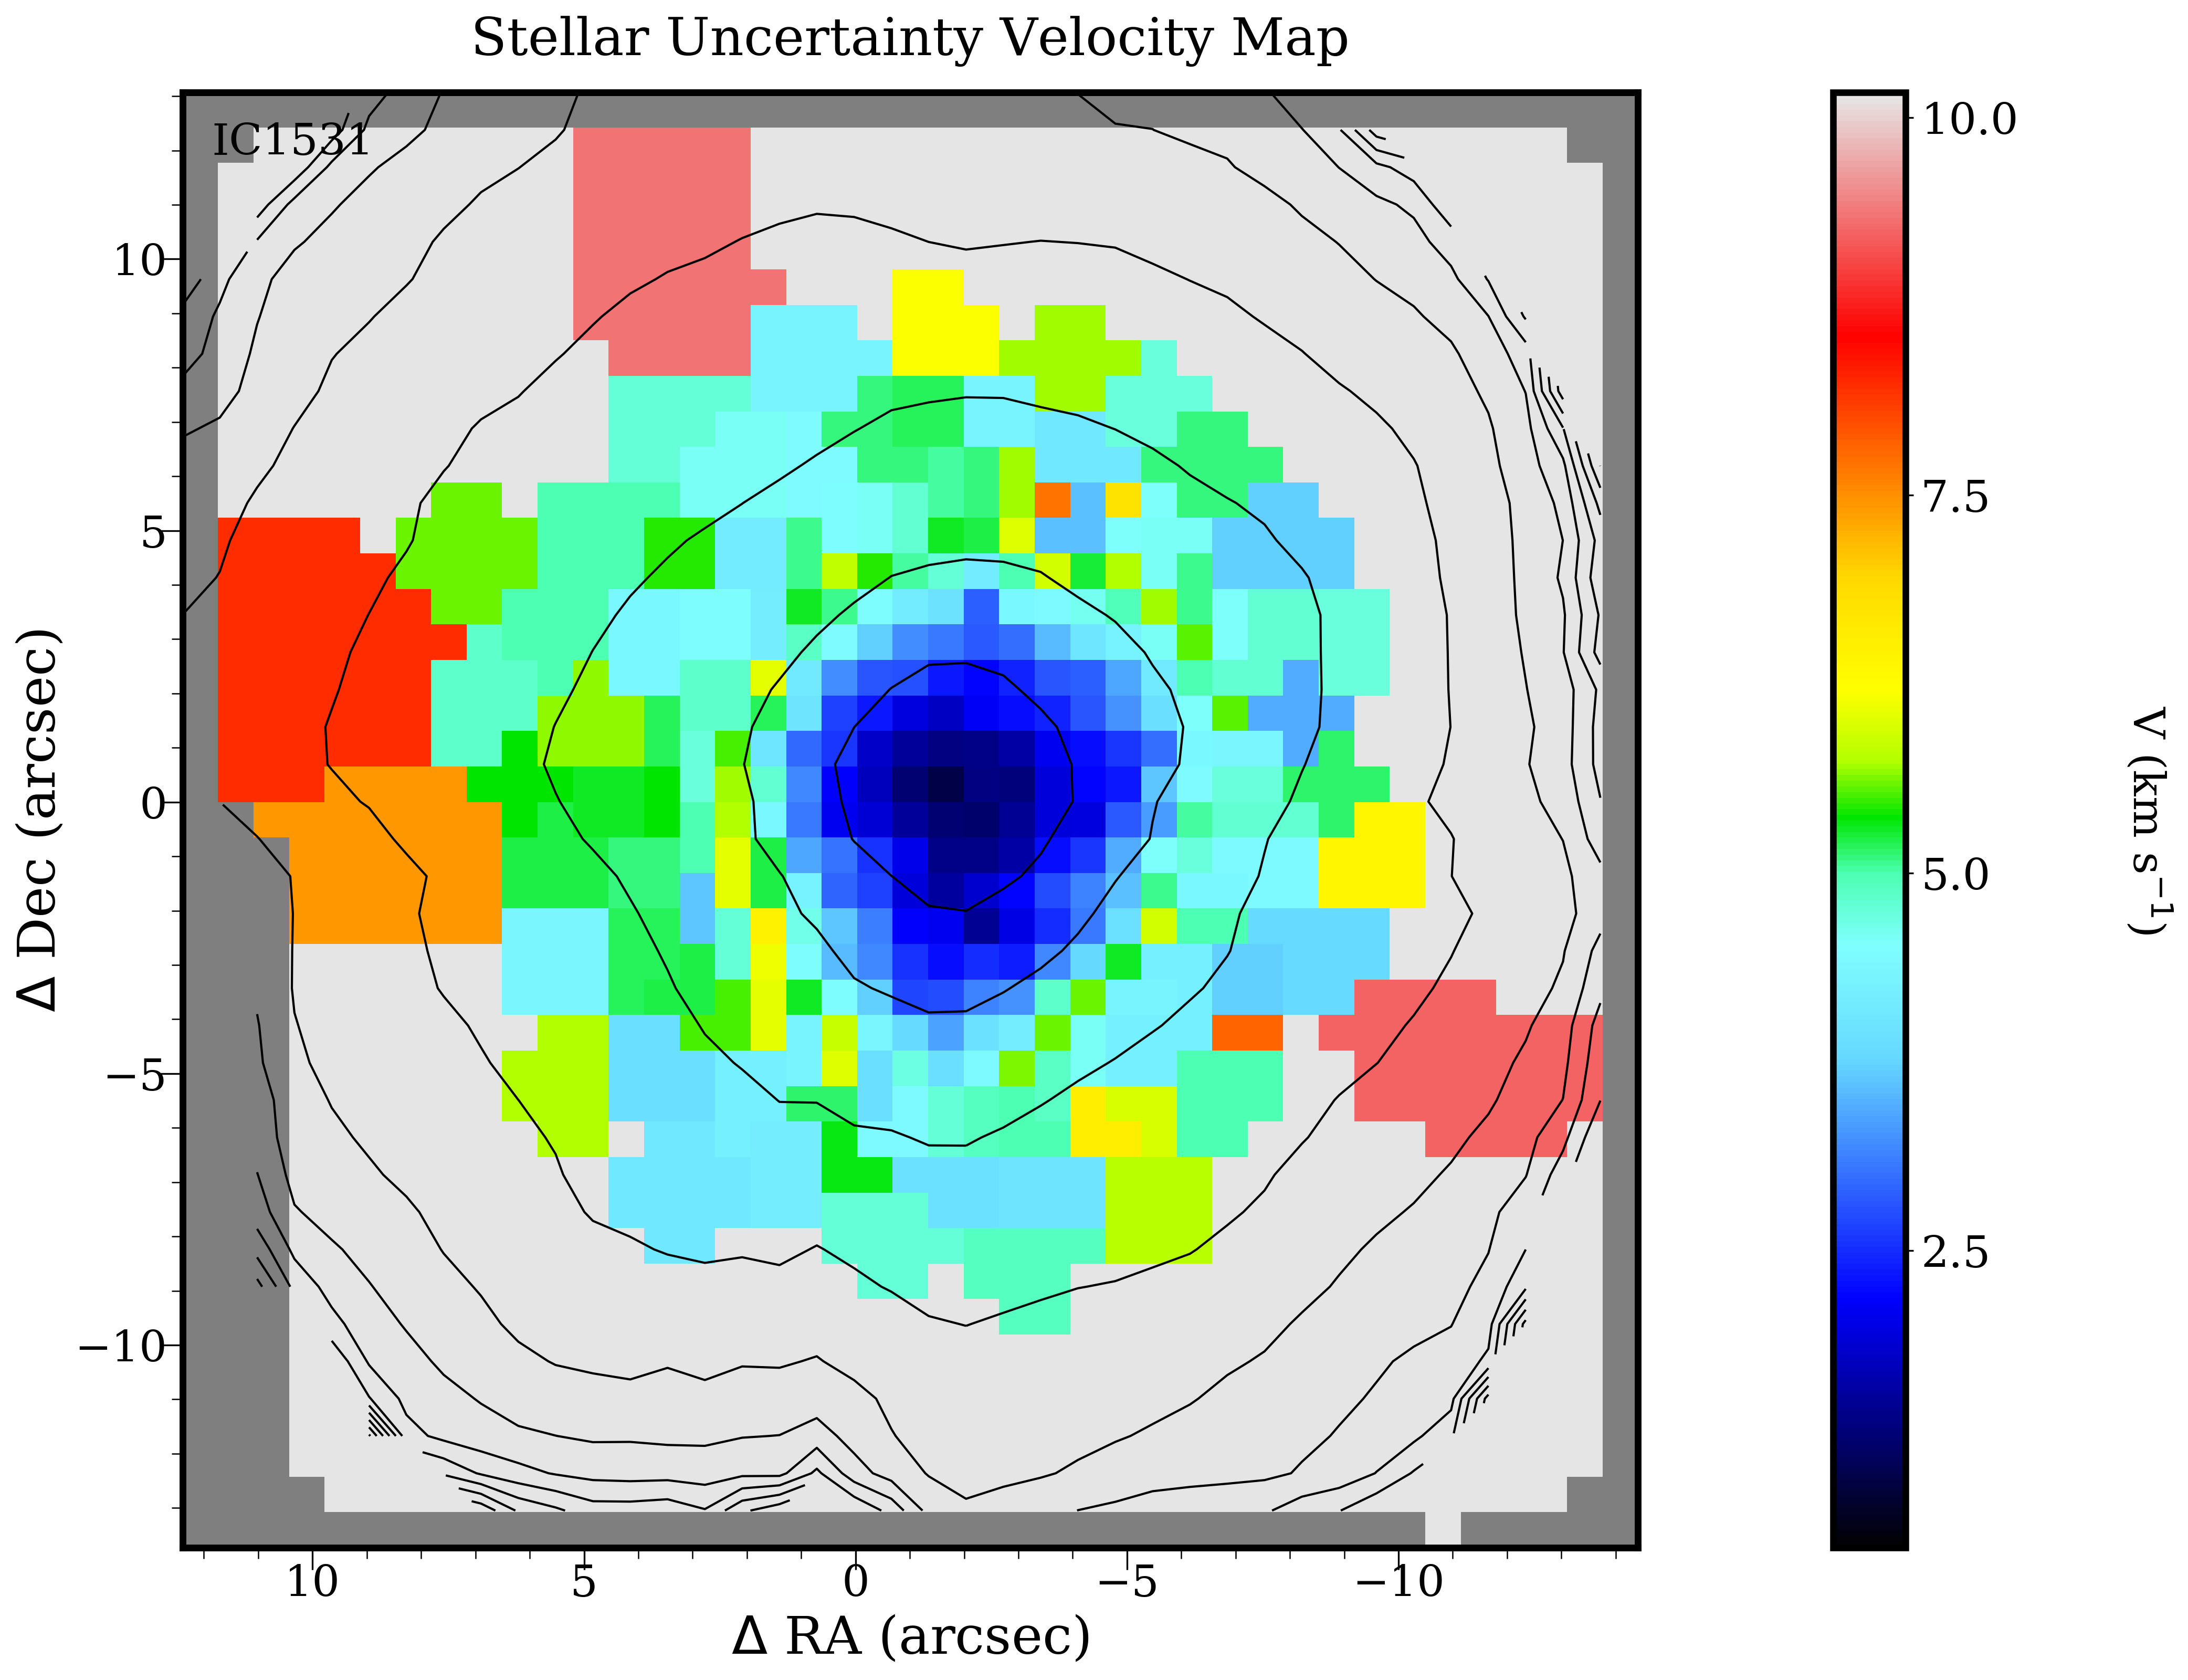
\includegraphics[width=0.245\textwidth]{Vmaps/ic1531_stellar_vel_uncert.png}
      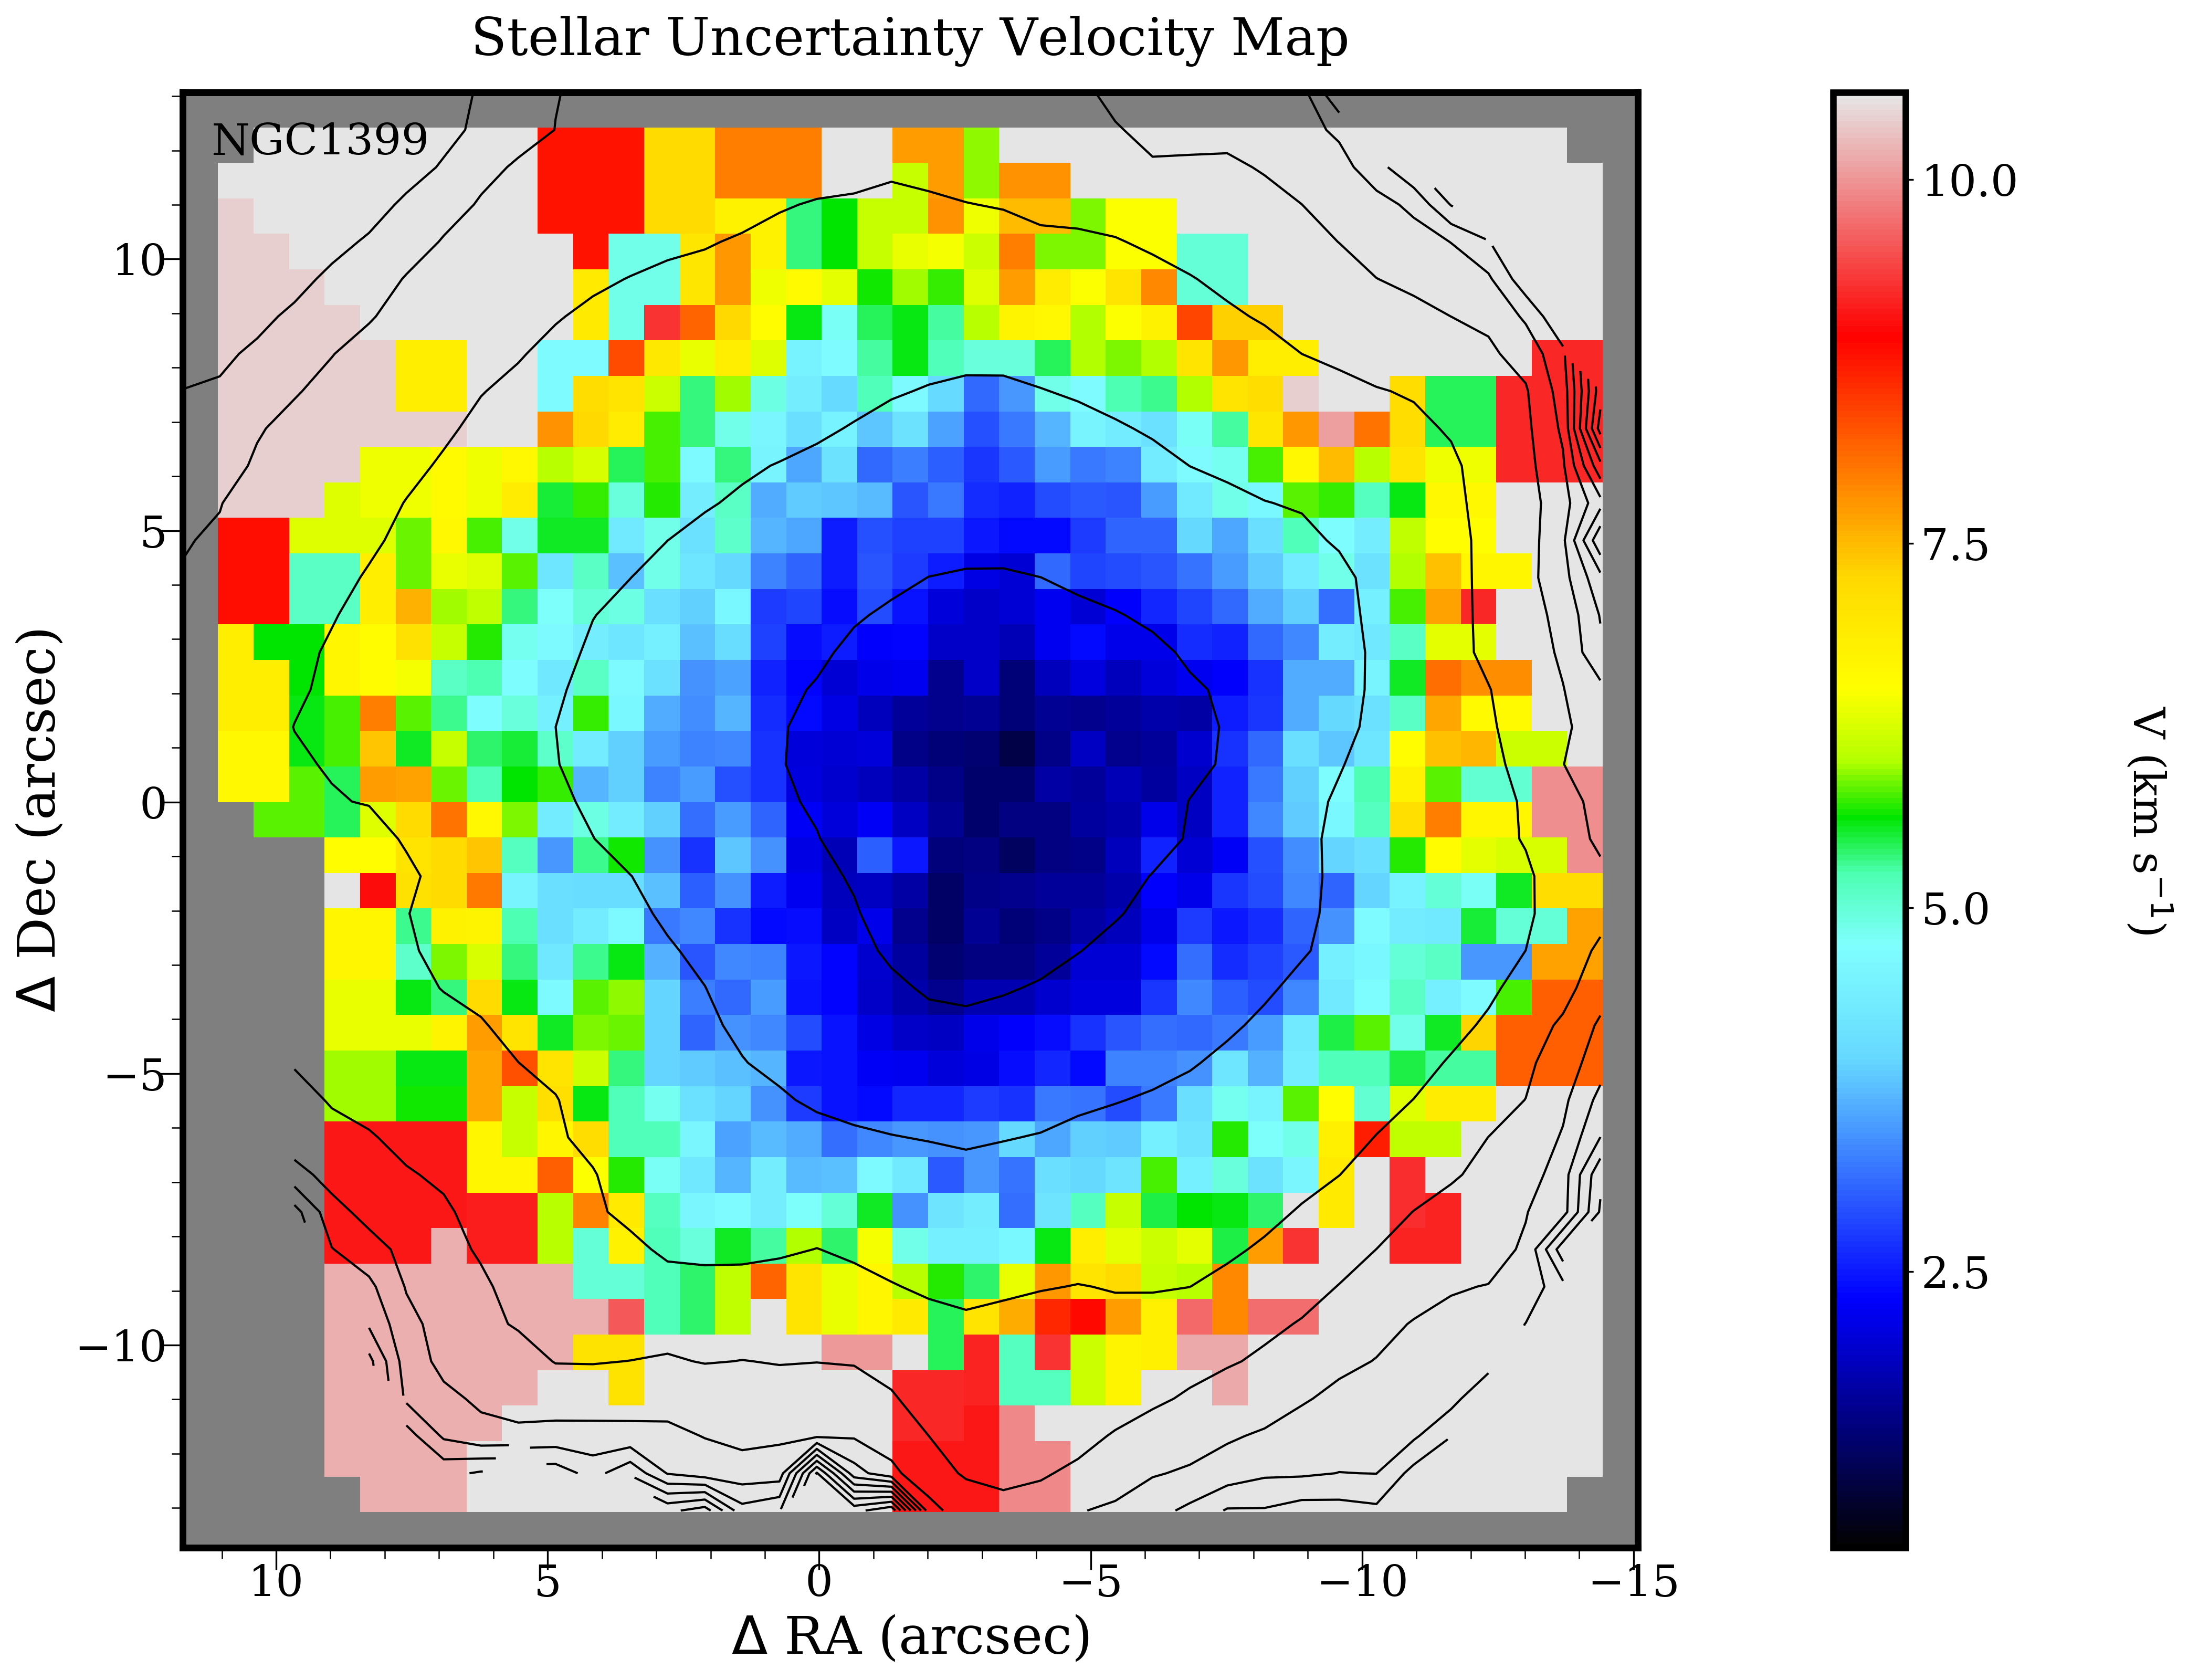
\includegraphics[width=0.245\textwidth]{Vmaps/ngc1399_stellar_vel_uncert.png}
      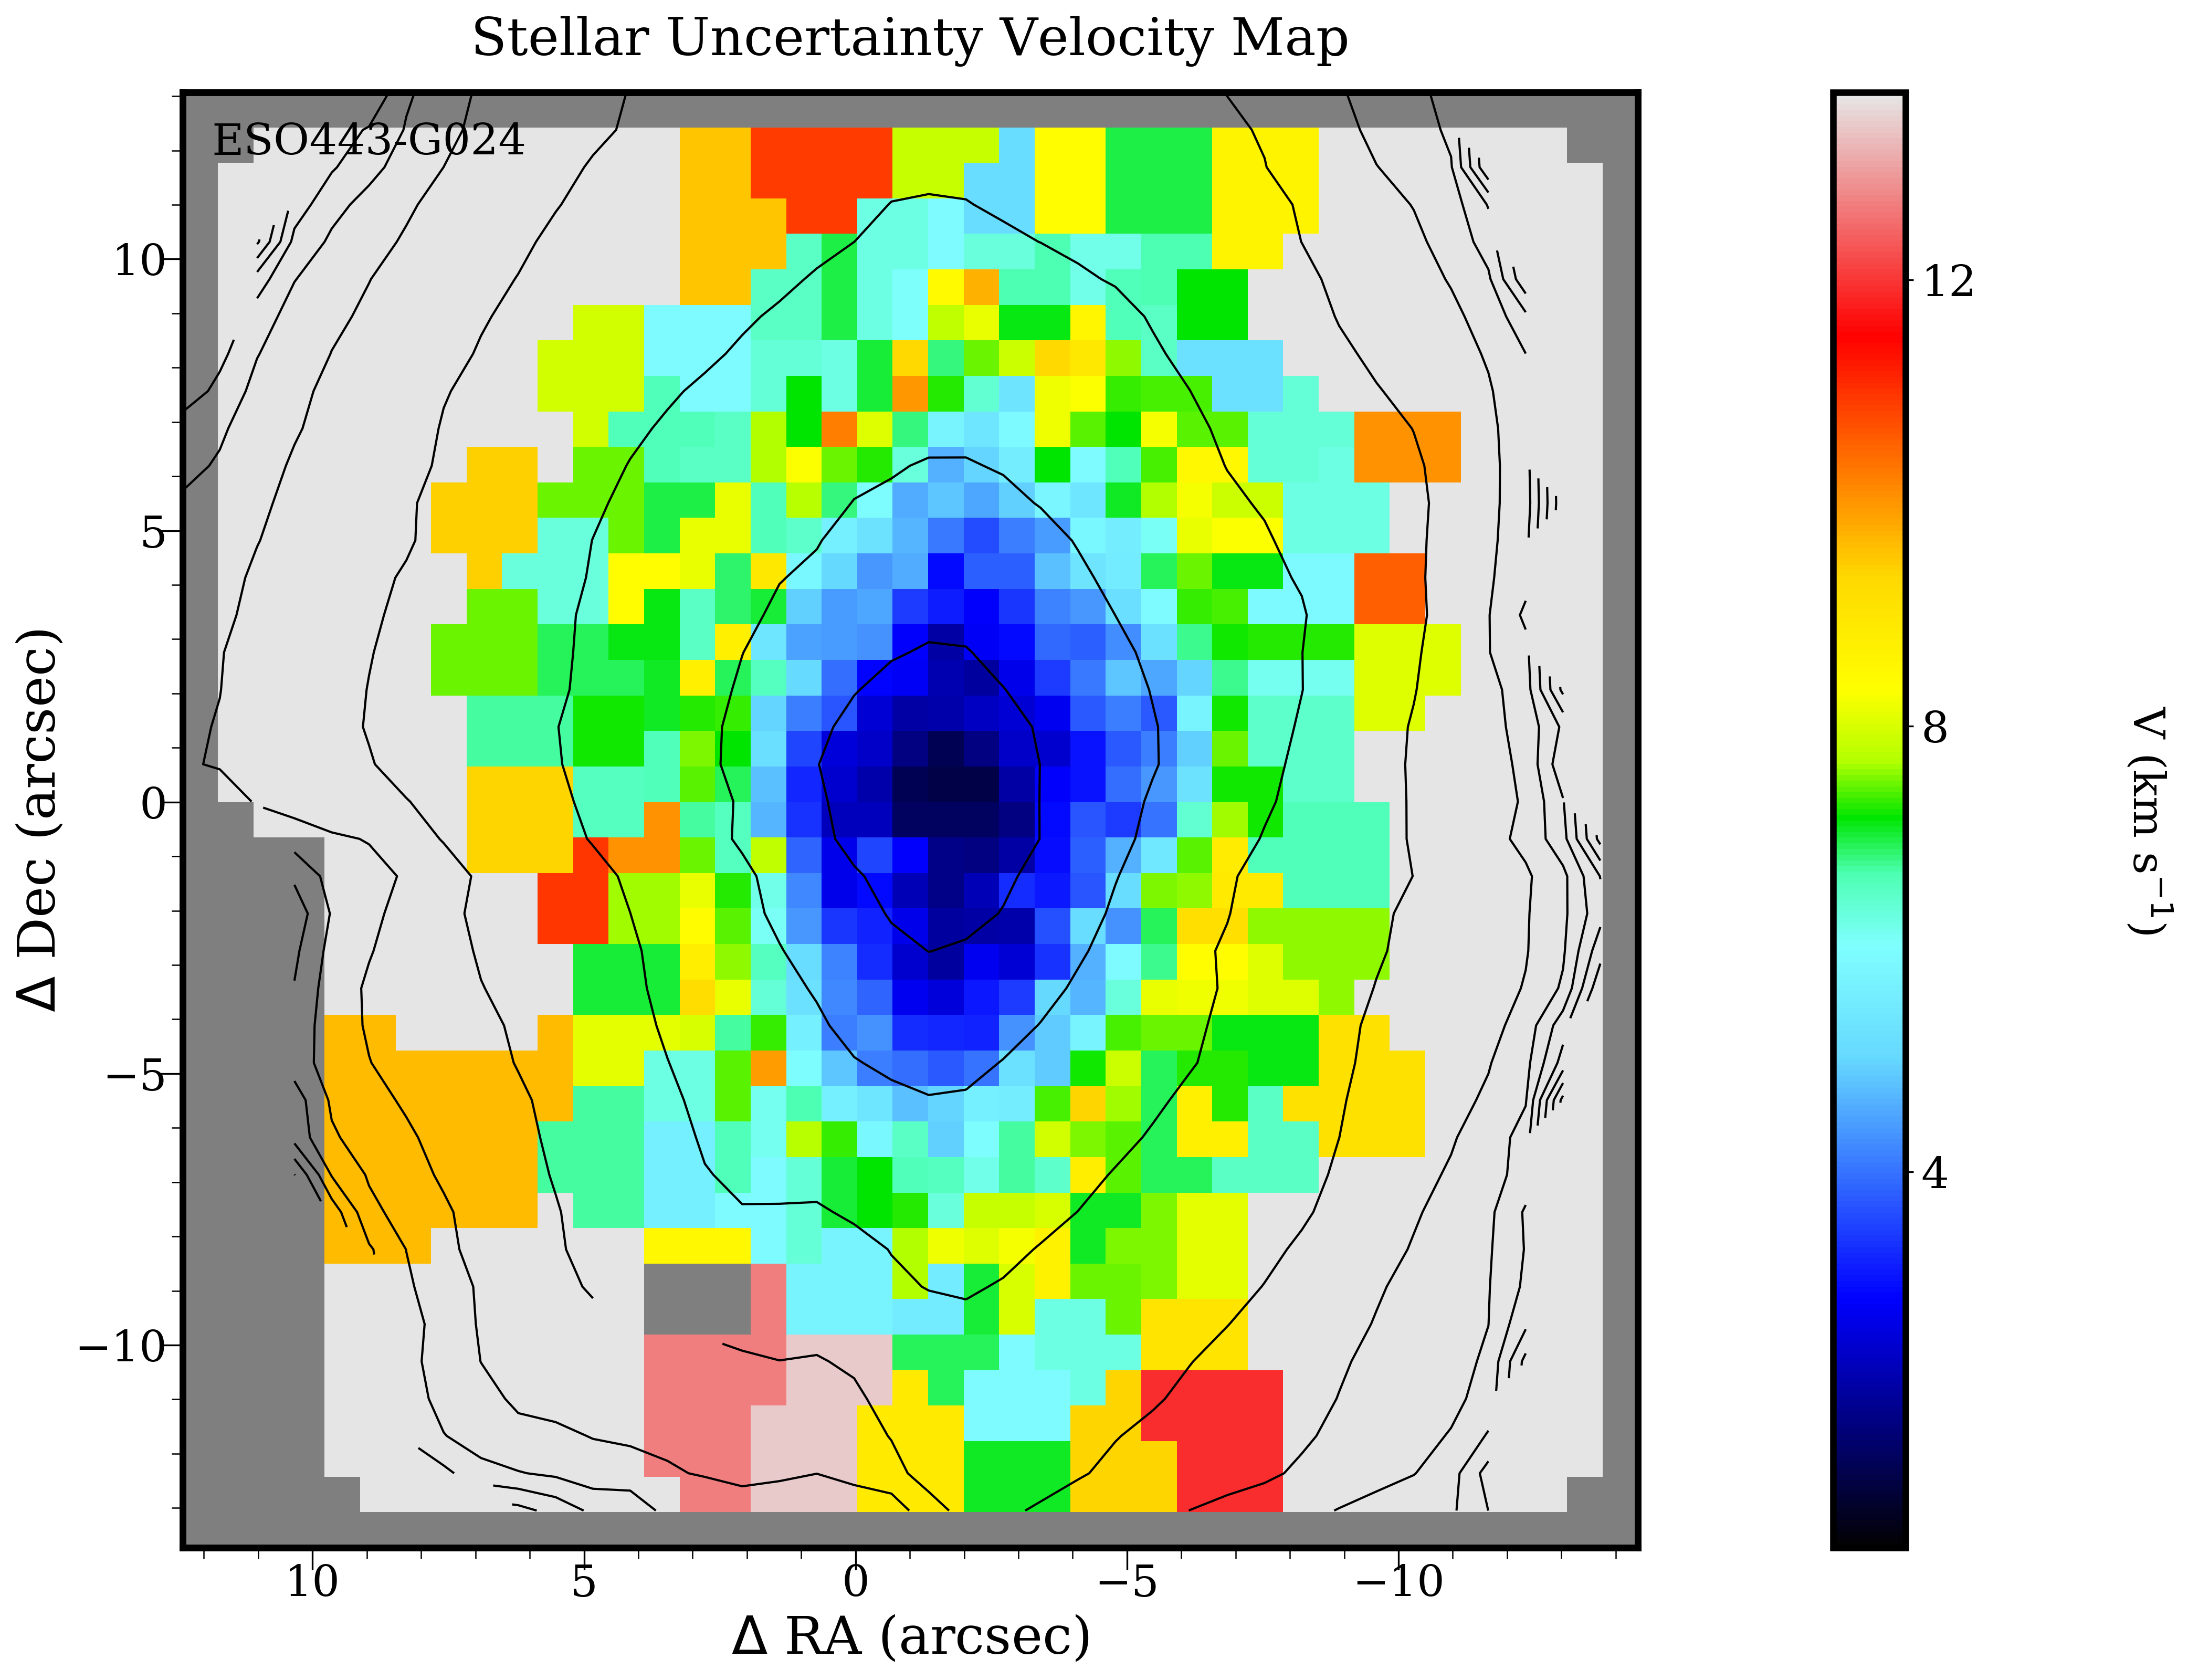
\includegraphics[width=0.245\textwidth]{Vmaps/eso443-g024_stellar_vel_uncert.png}
      \caption[VIMOS velocity uncertocity maps]{Uncertainties in the velocity for each galaxy in the VIMOS sample. Plots are ordered and contour colors are as in figure \ref{fig:Vstellar_img}}
      \label{fig:Vstellar_vel_uncert}
\end{figure*}

\begin{figure*}
      \centering
      \includegraphics[width=0.245\textwidth]{Vmaps/ngc0612_stellar_sigma.png}
      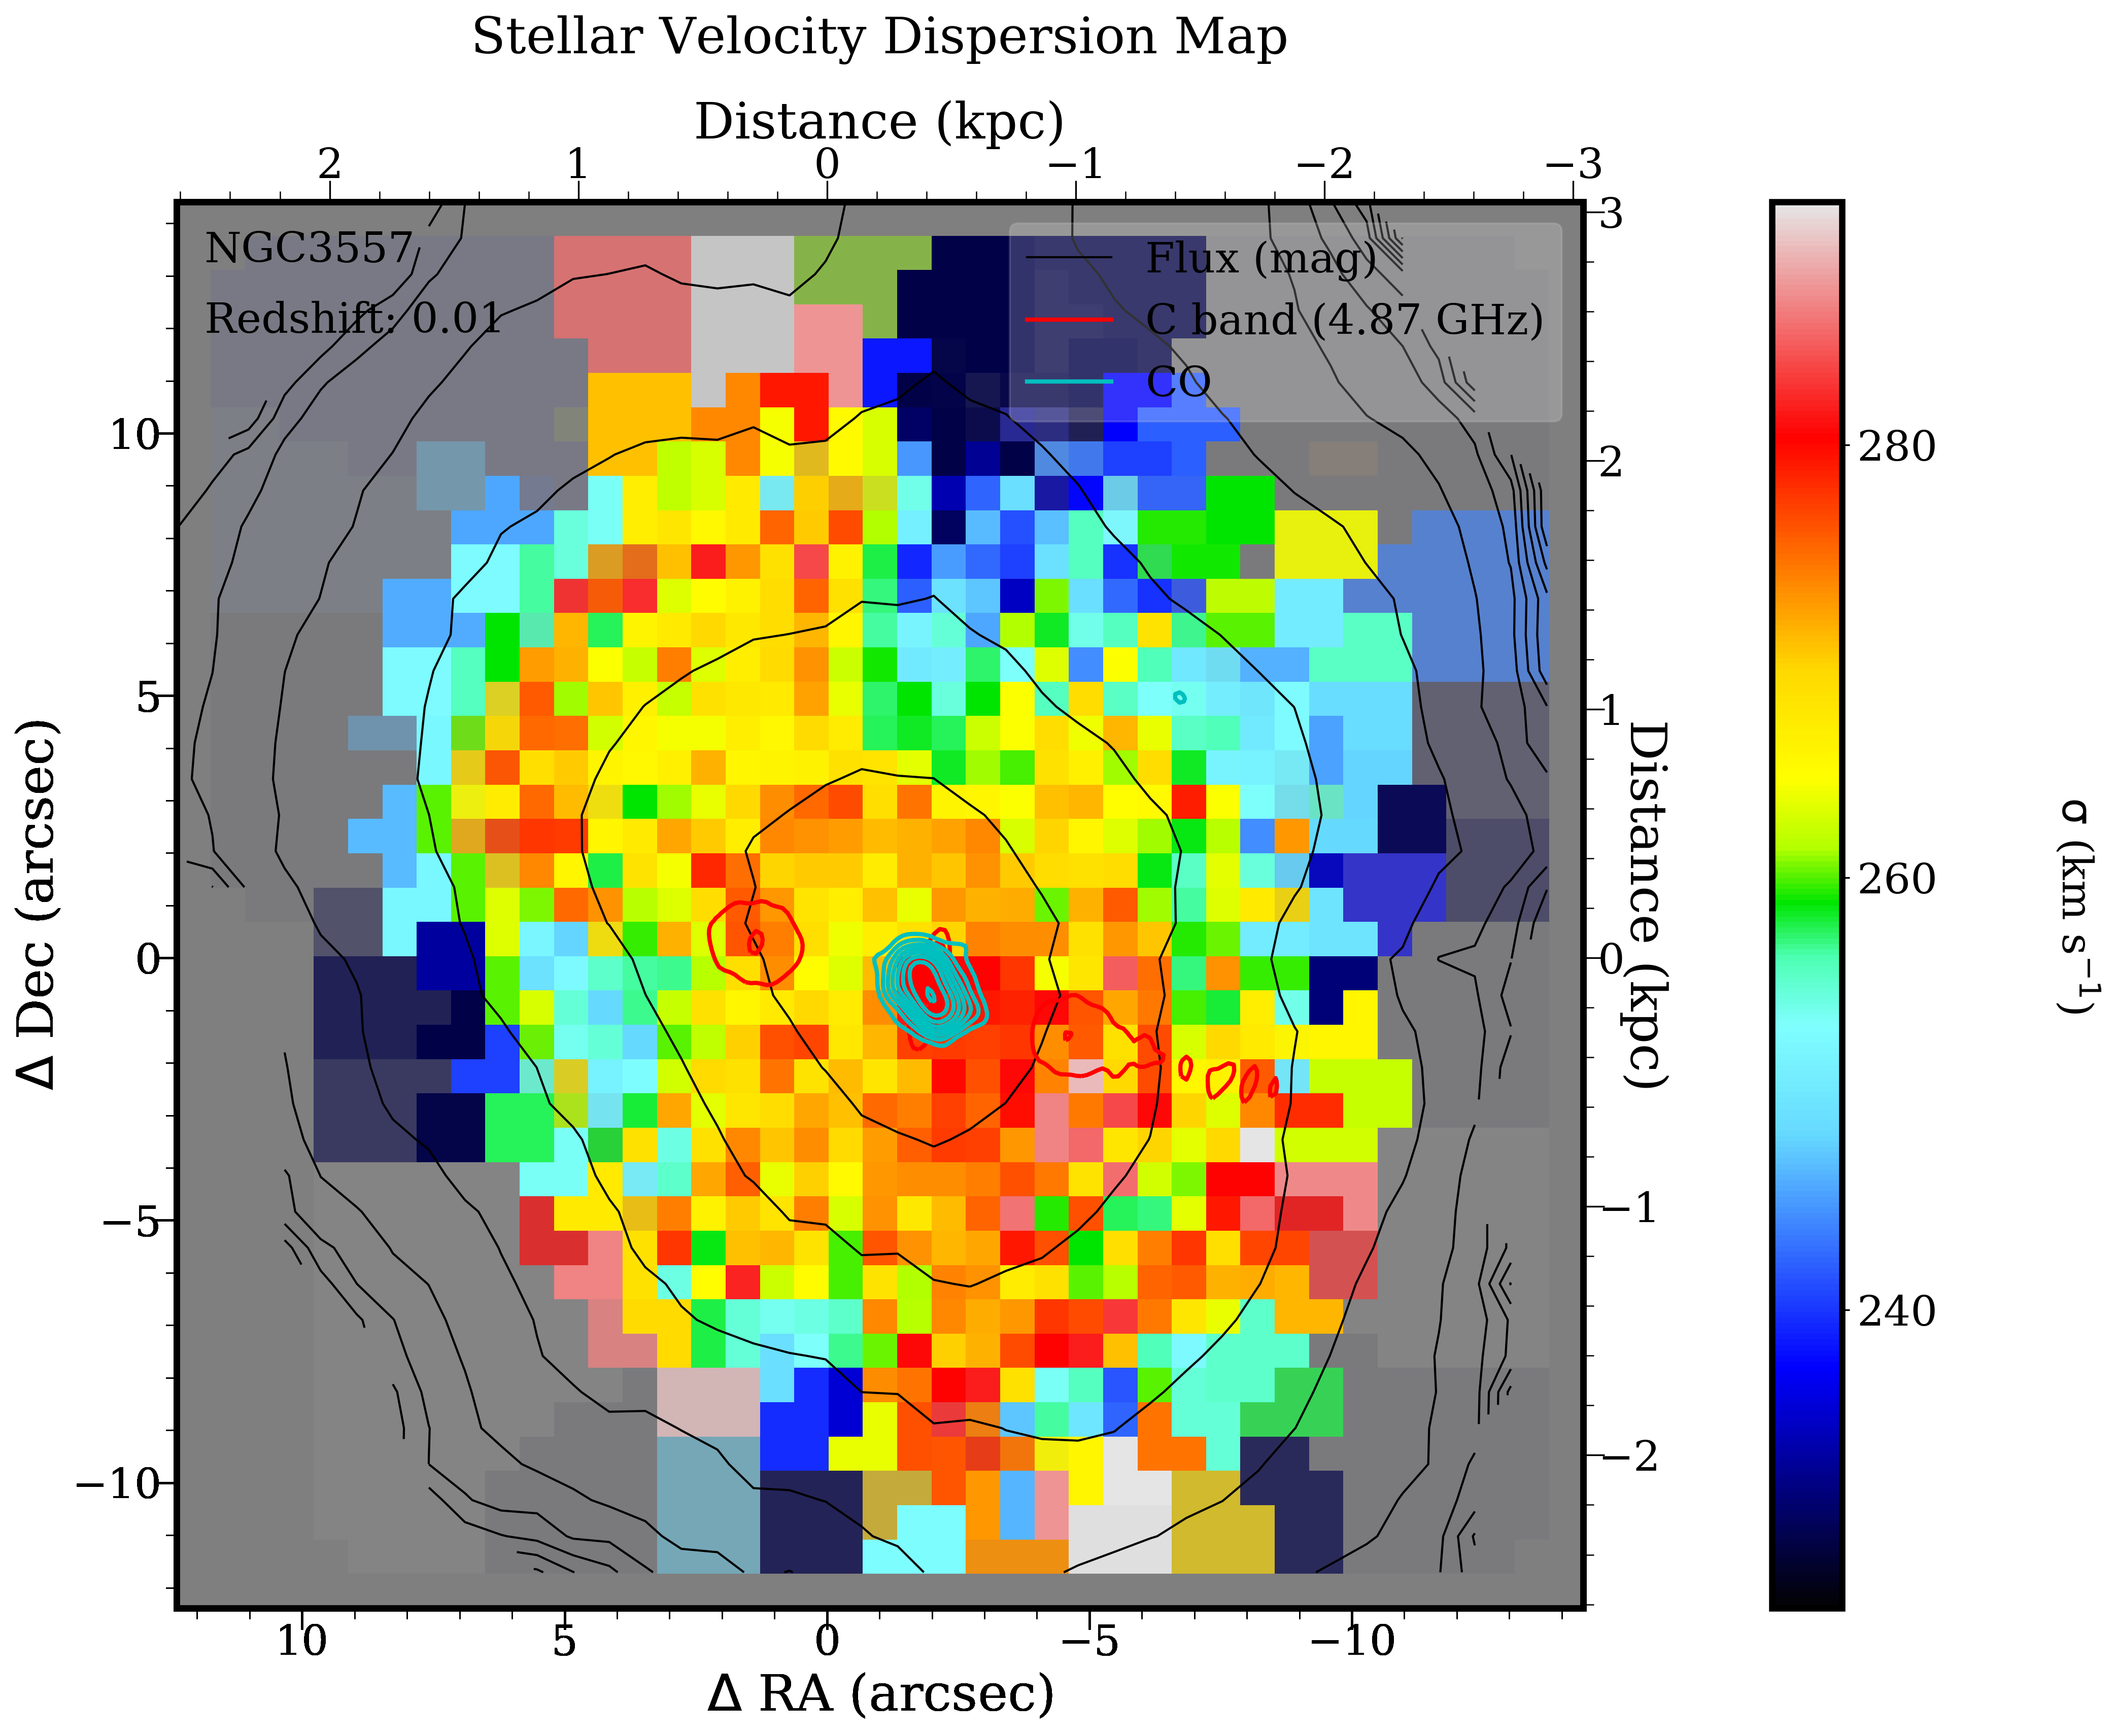
\includegraphics[width=0.245\textwidth]{Vmaps/ngc3557_stellar_sigma.png}
      \includegraphics[width=0.245\textwidth]{Vmaps/ngc3100_stellar_sigma.png}
      \includegraphics[width=0.245\textwidth]{Vmaps/ic1459_stellar_sigma.png}
      \includegraphics[width=0.245\textwidth]{Vmaps/pks0718-34_stellar_sigma.png}
      \includegraphics[width=0.245\textwidth]{Vmaps/ic4296_stellar_sigma.png}
      \includegraphics[width=0.245\textwidth]{Vmaps/ngc7075_stellar_sigma.png}
      \includegraphics[width=0.245\textwidth]{Vmaps/ic1531_stellar_sigma.png}
      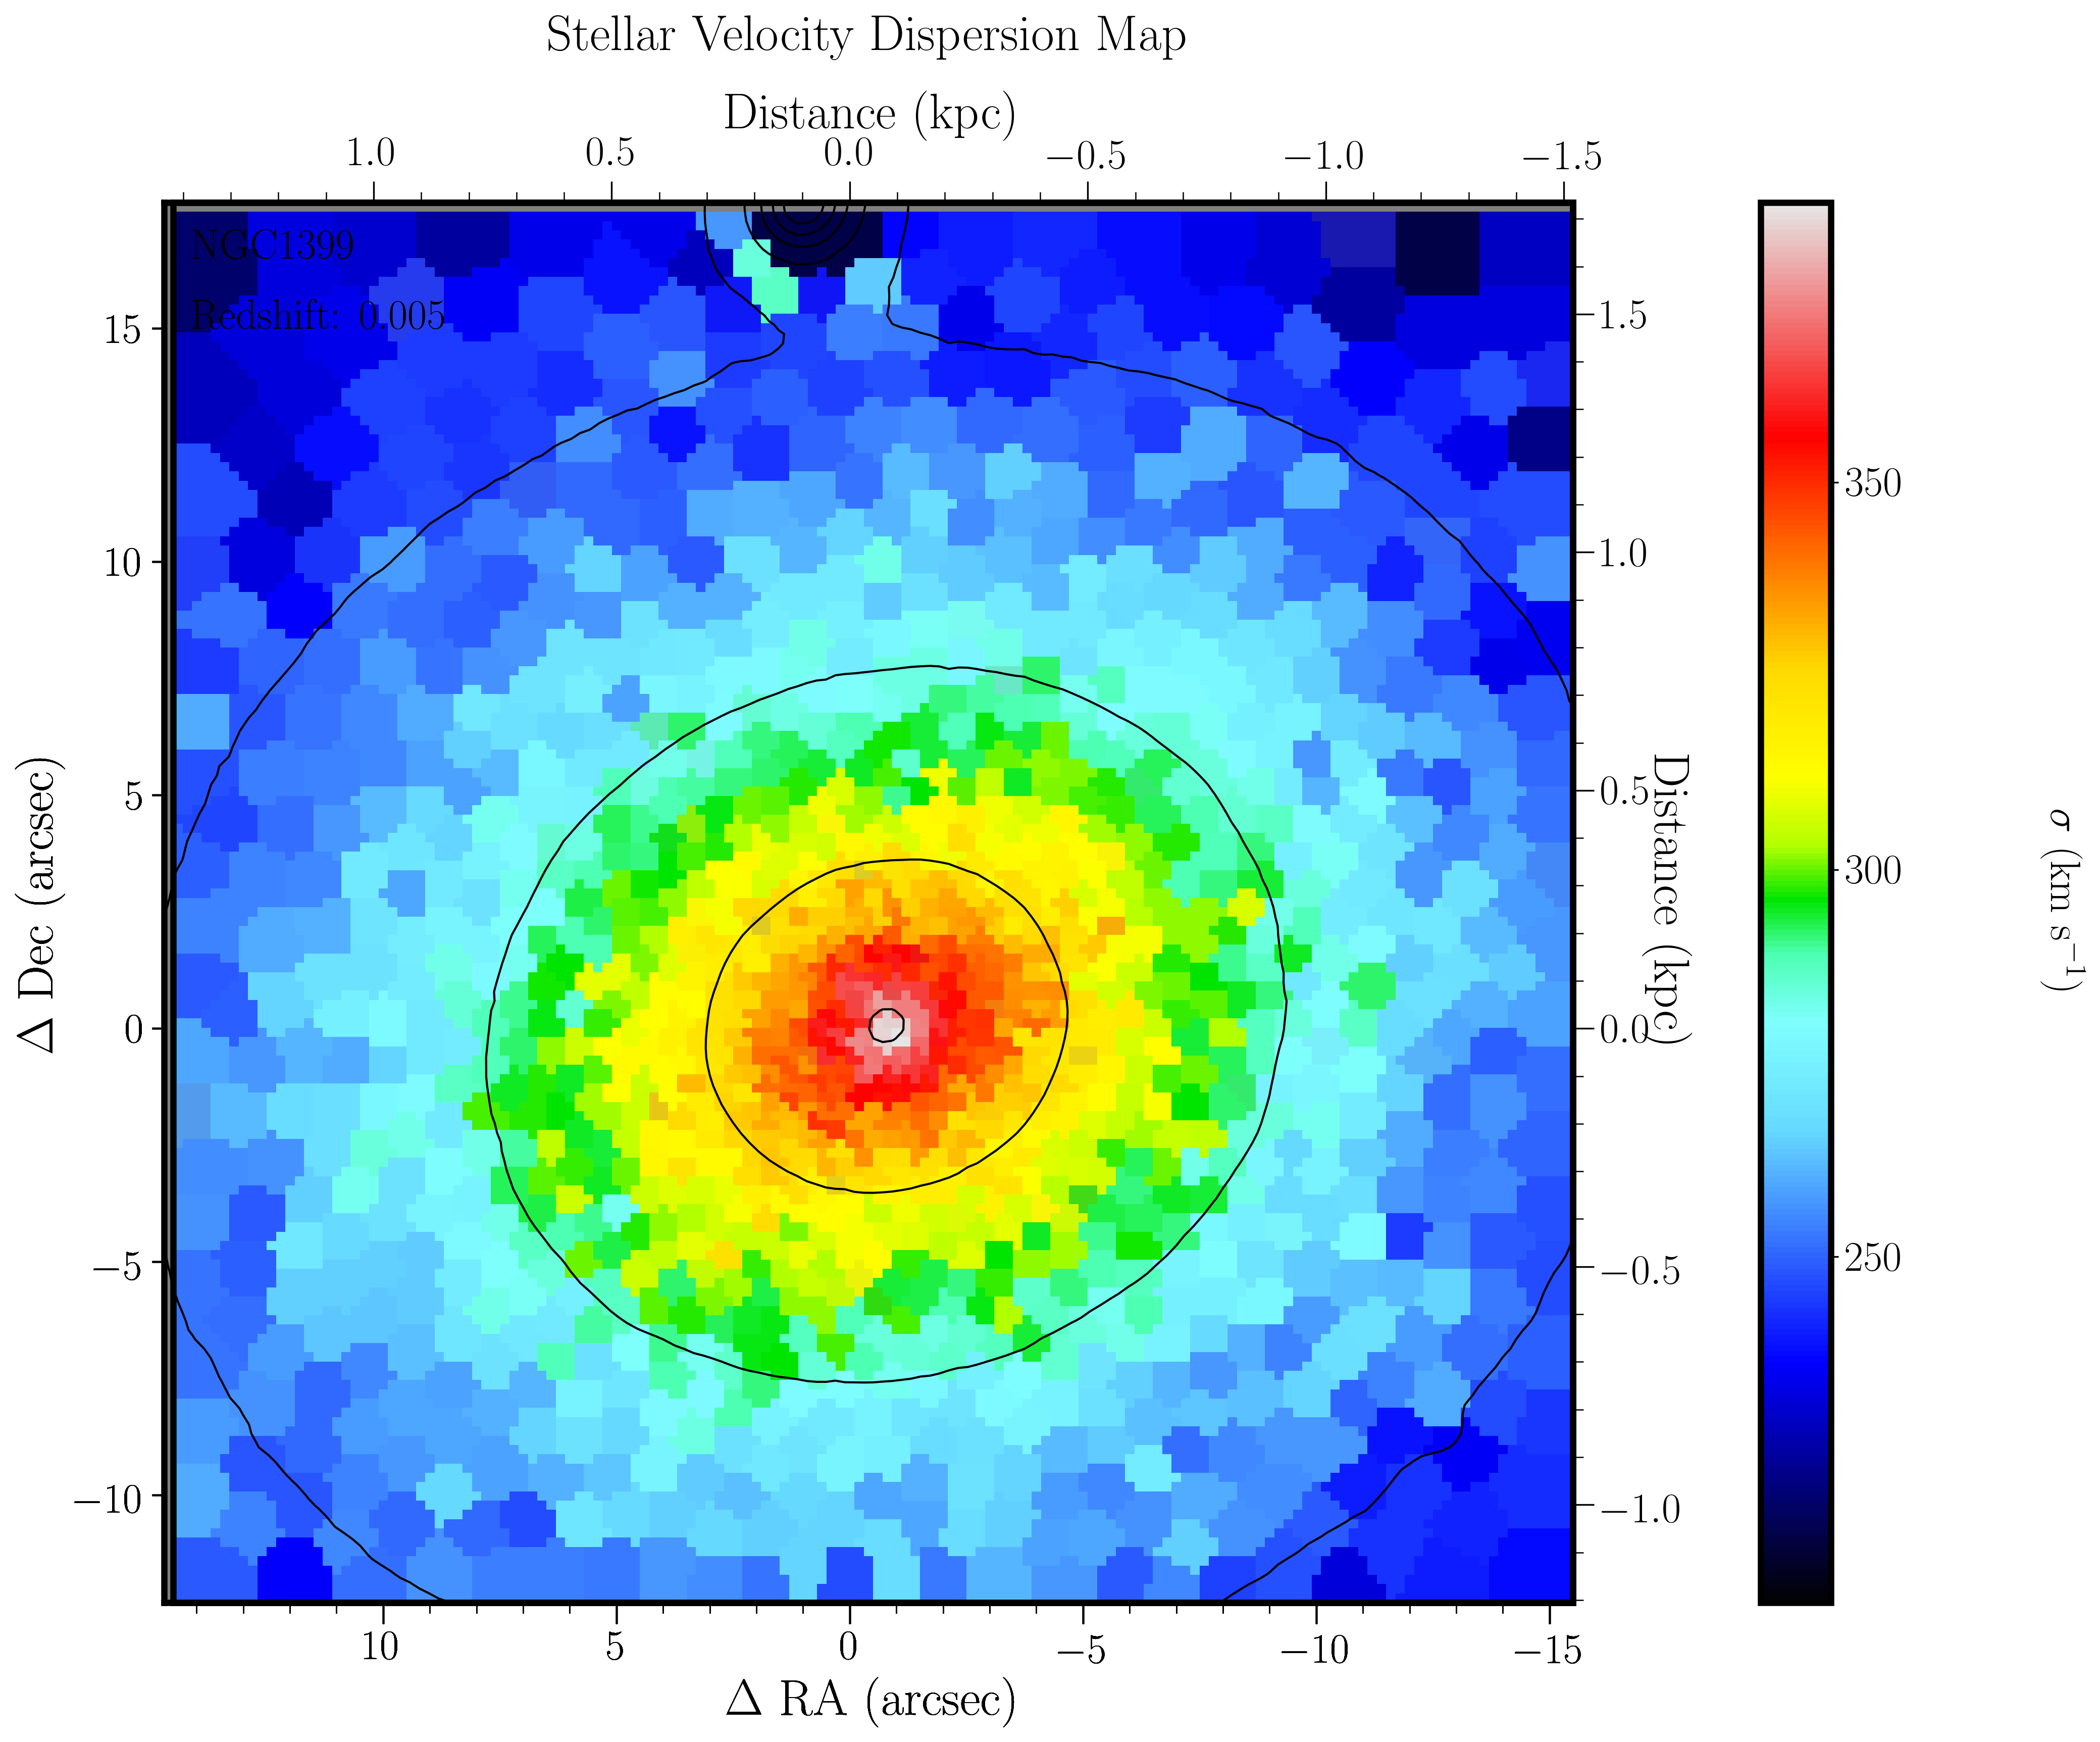
\includegraphics[width=0.245\textwidth]{Vmaps/ngc1399_stellar_sigma.png}
      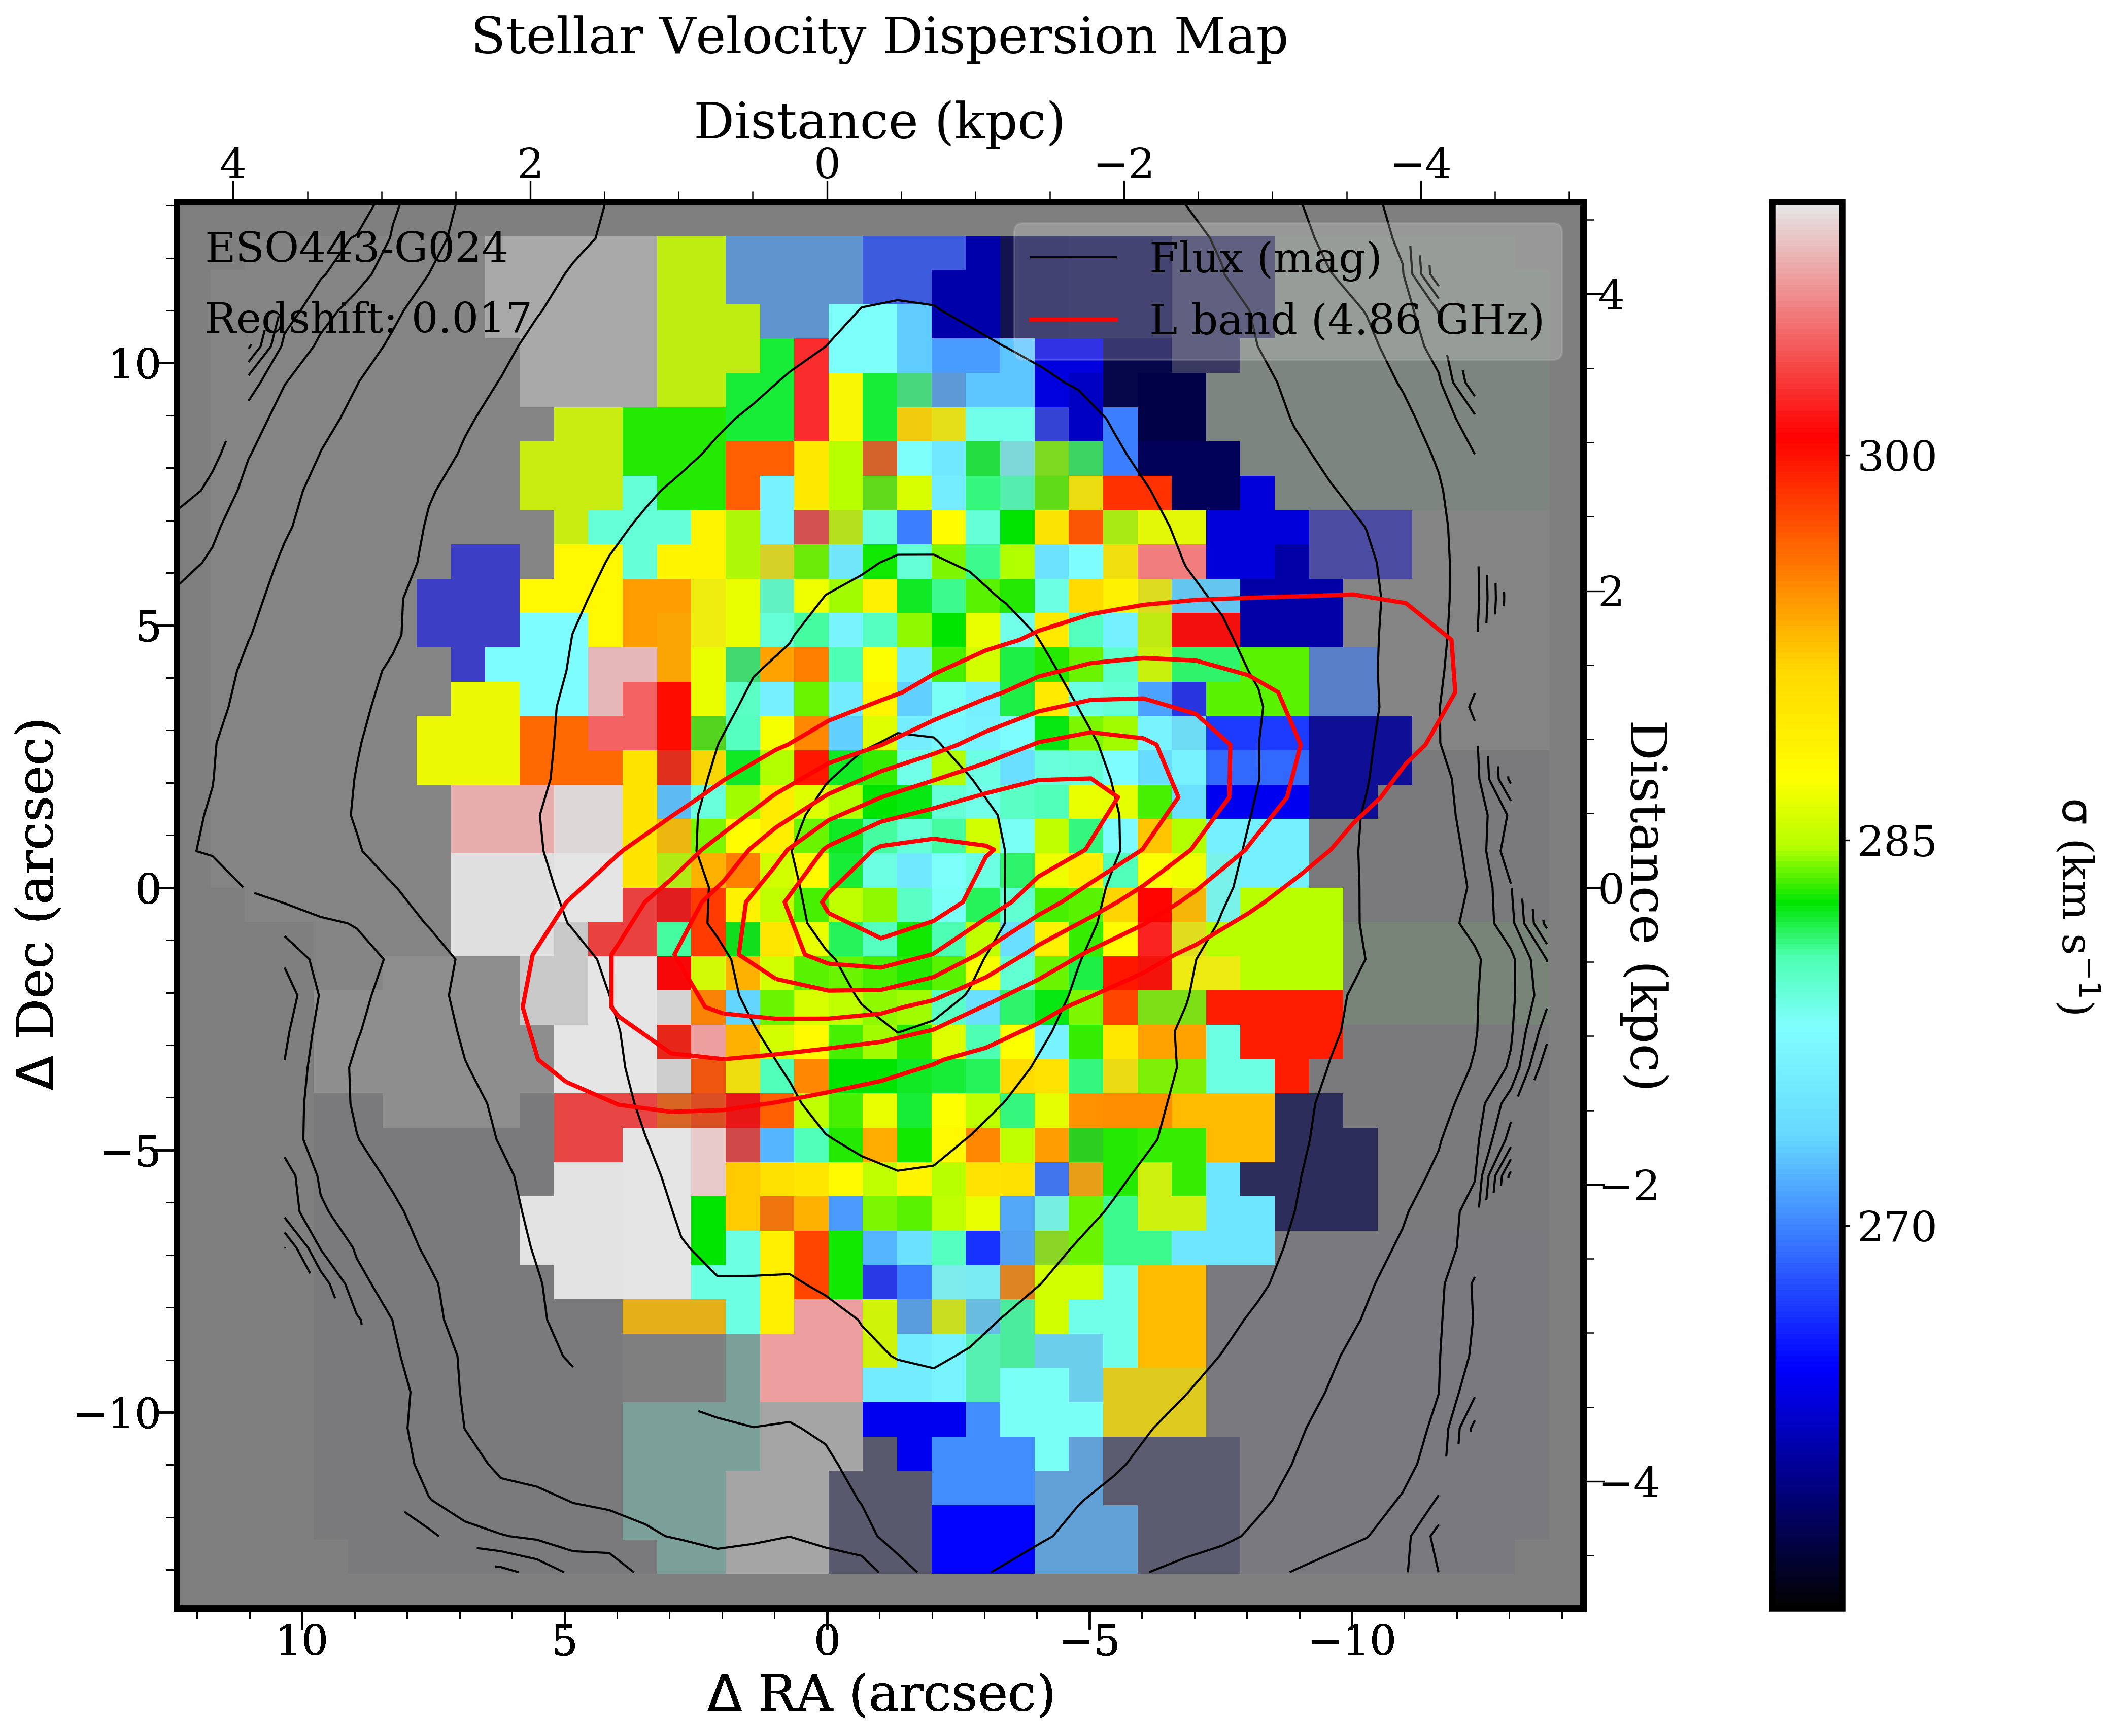
\includegraphics[width=0.245\textwidth]{Vmaps/eso443-g024_stellar_sigma.png}
      \caption[VIMOS velocity dispersion]{Velocity dispersion for each galaxy in the VIMOS sample. Plots are ordered and contour colors are as in figure \ref{fig:Vstellar_img}}
      \label{fig:Vstellar_sigma}
\end{figure*}


\begin{figure*}
      \centering
      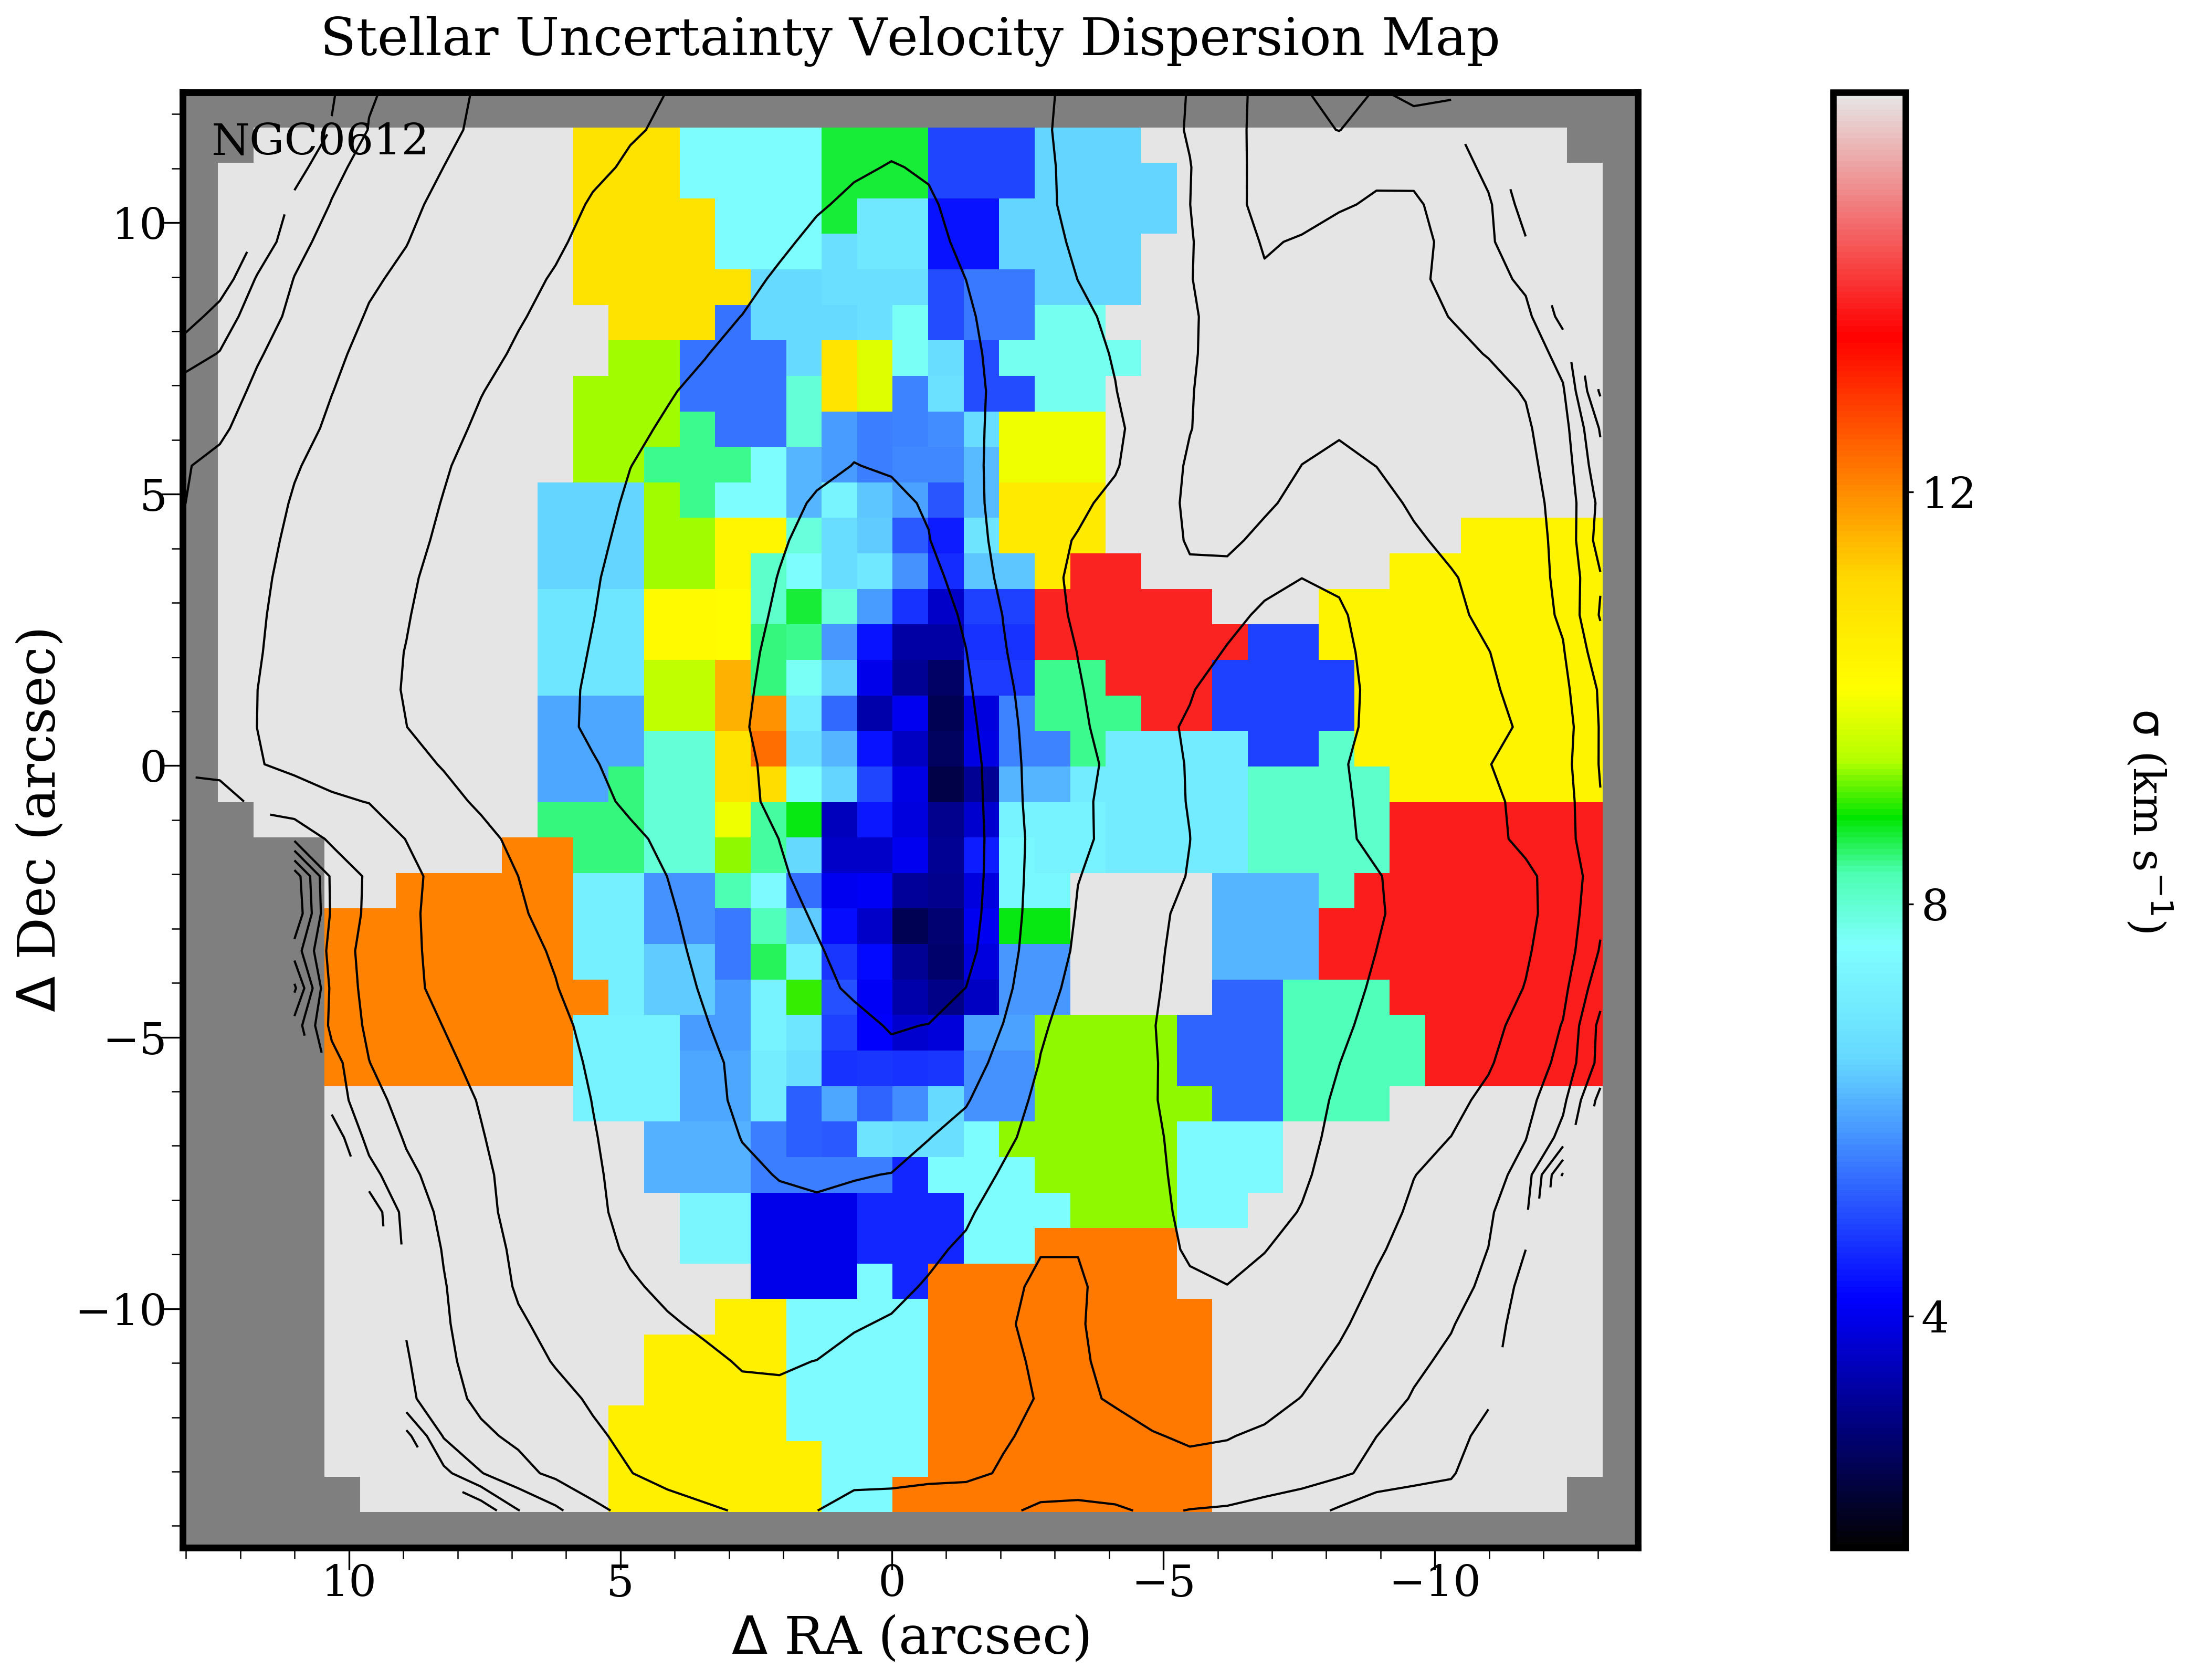
\includegraphics[width=0.245\textwidth]{Vmaps/ngc0612_stellar_sigma_uncert.png}
      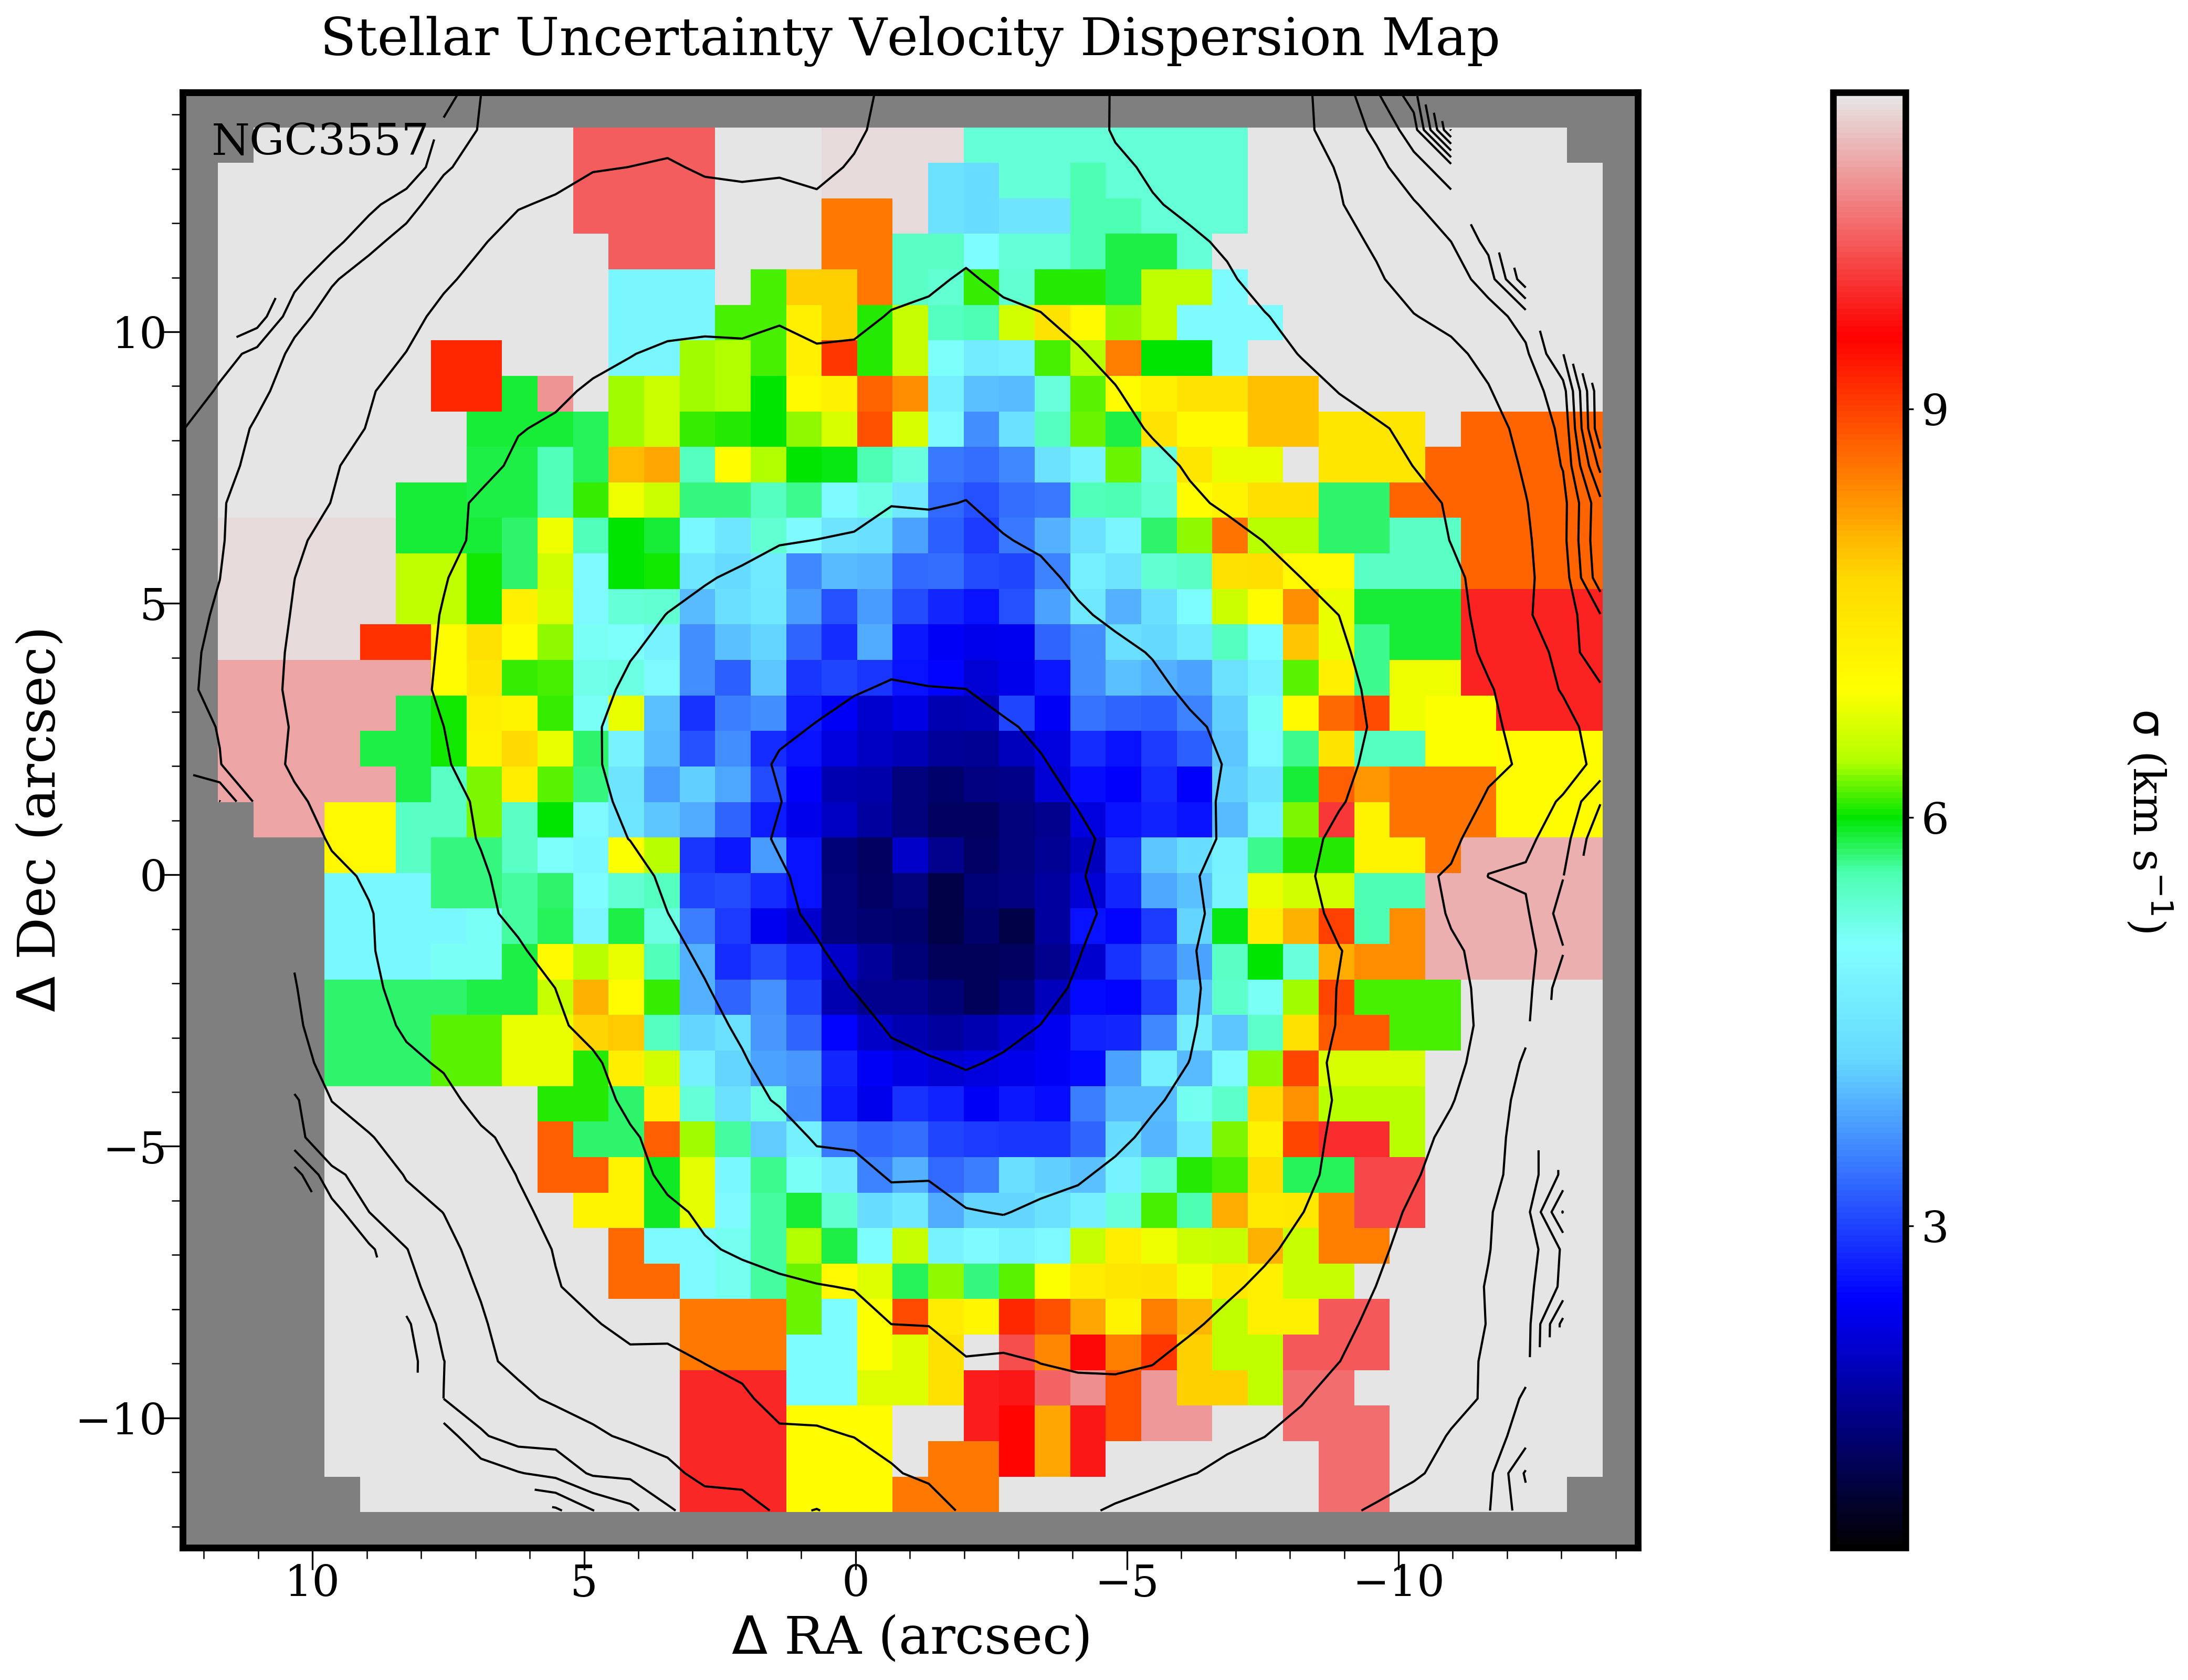
\includegraphics[width=0.245\textwidth]{Vmaps/ngc3557_stellar_sigma_uncert.png}
      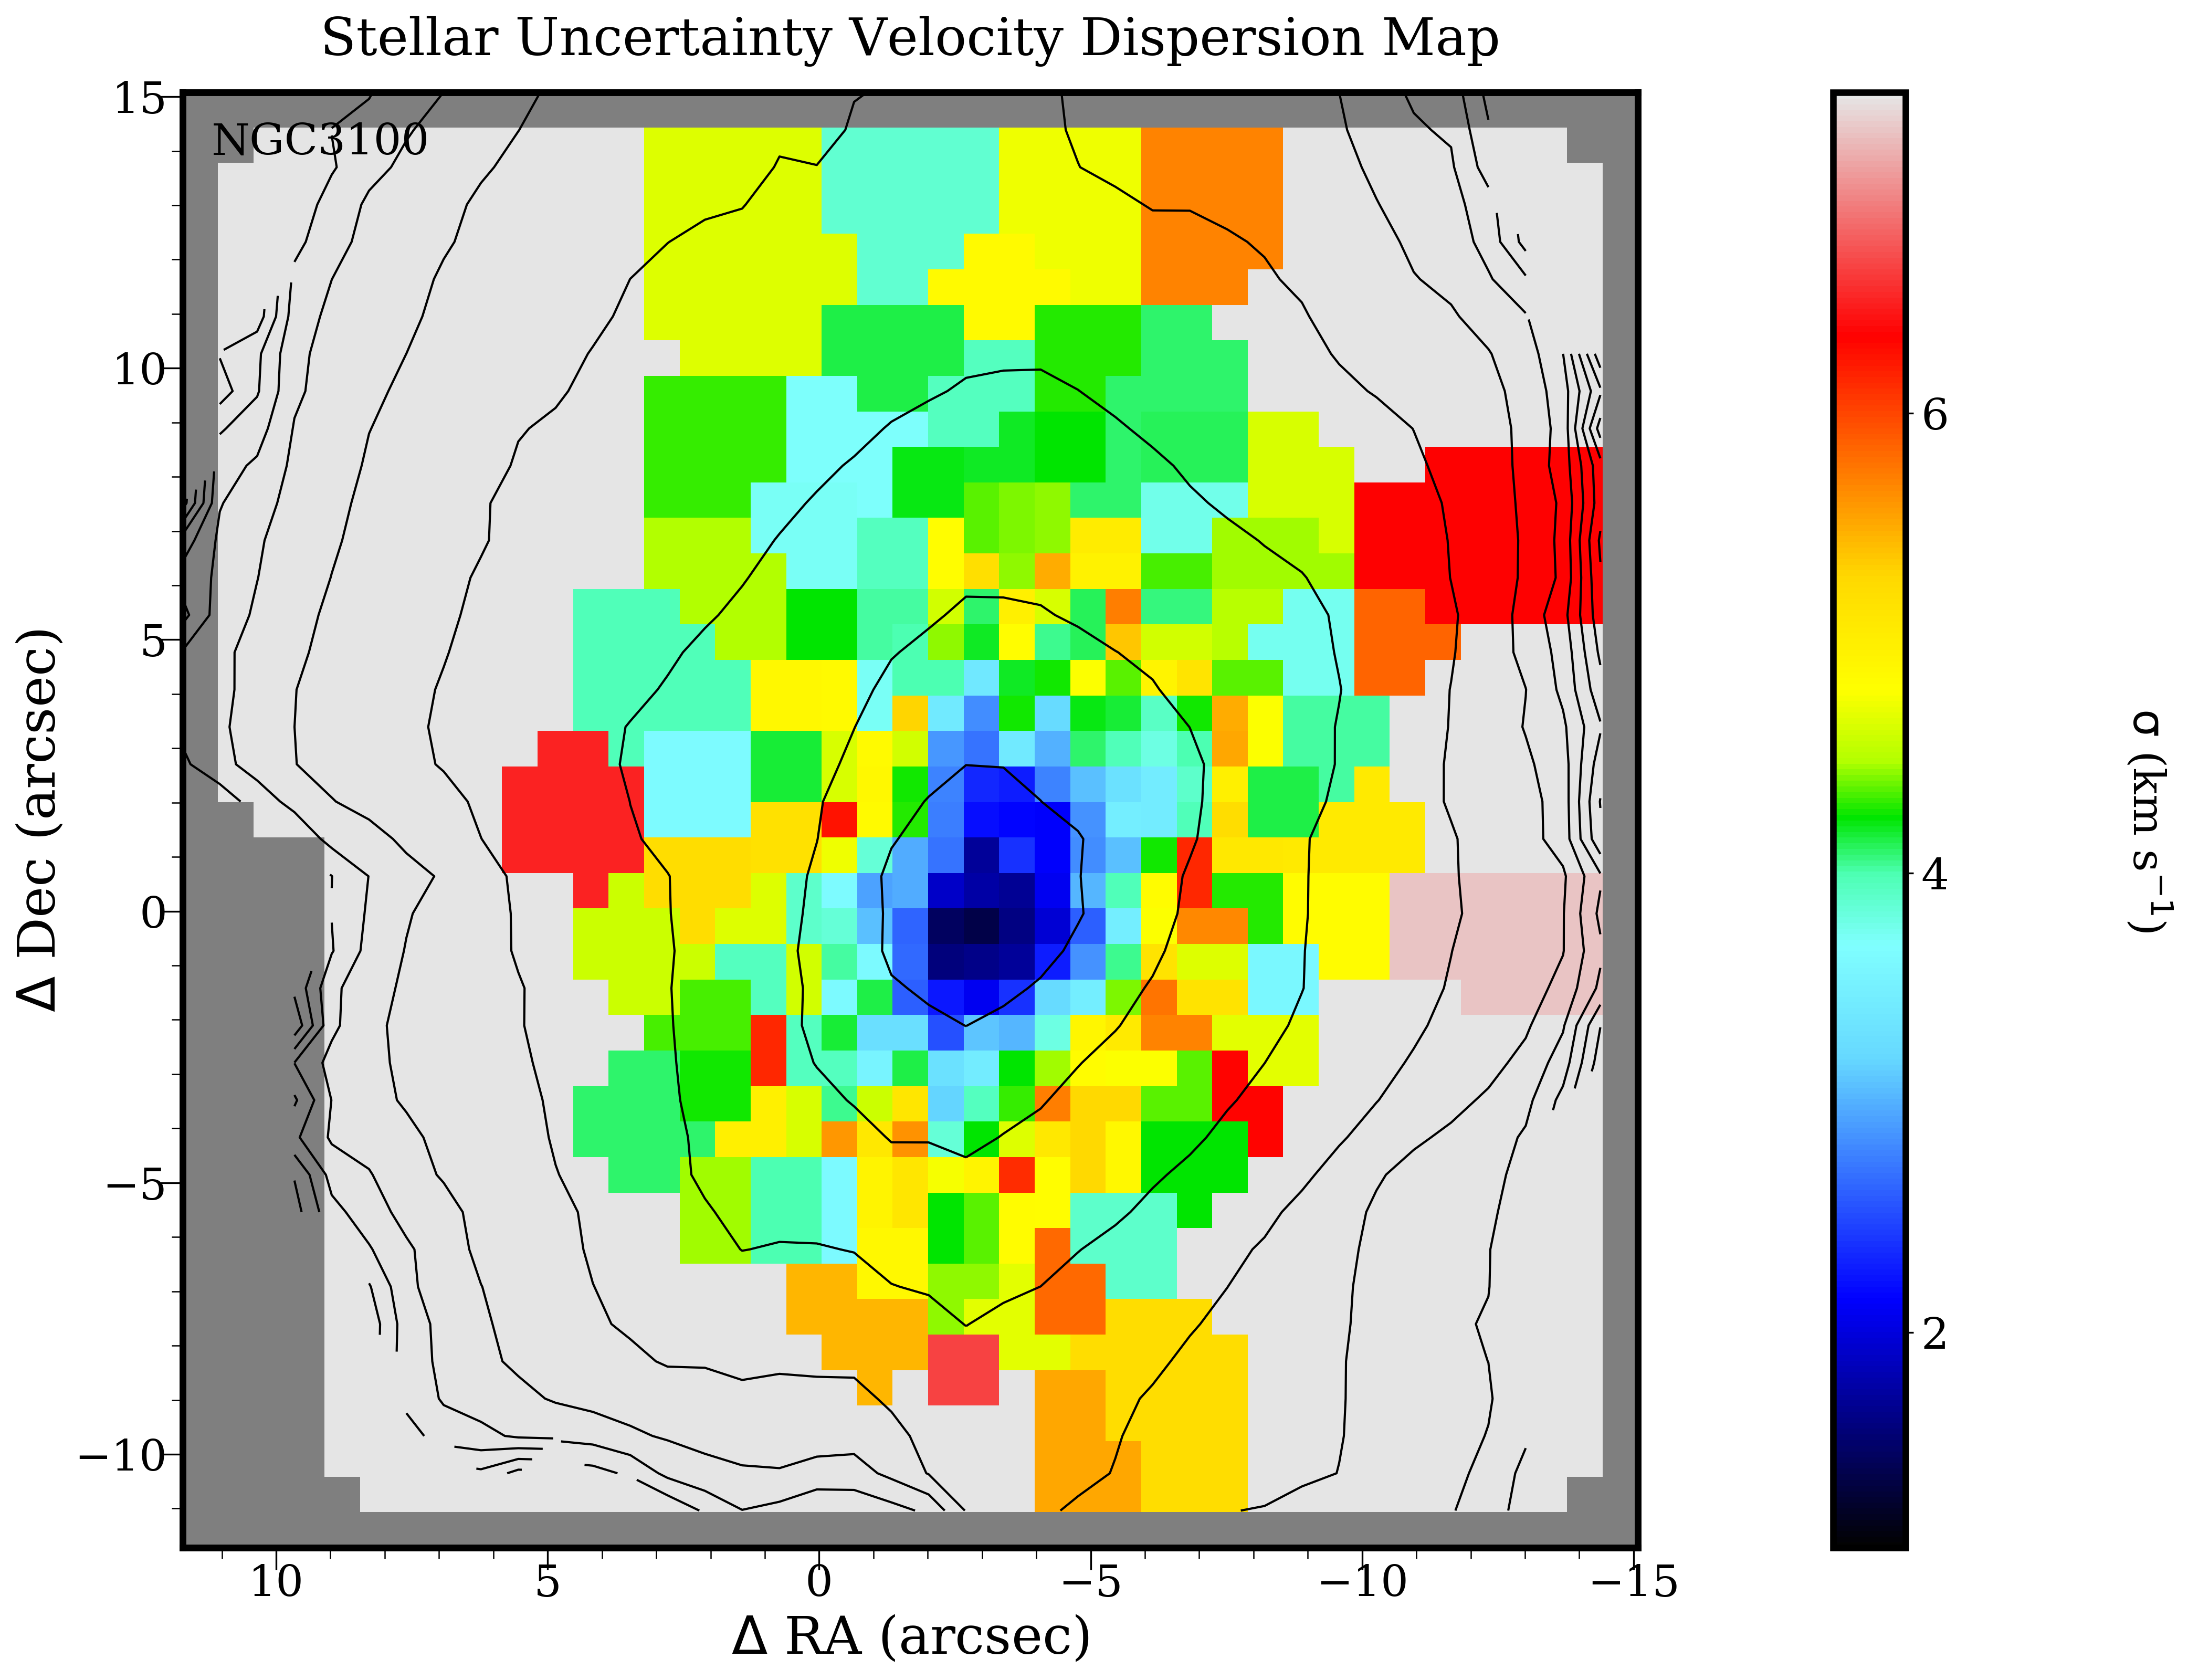
\includegraphics[width=0.245\textwidth]{Vmaps/ngc3100_stellar_sigma_uncert.png}
      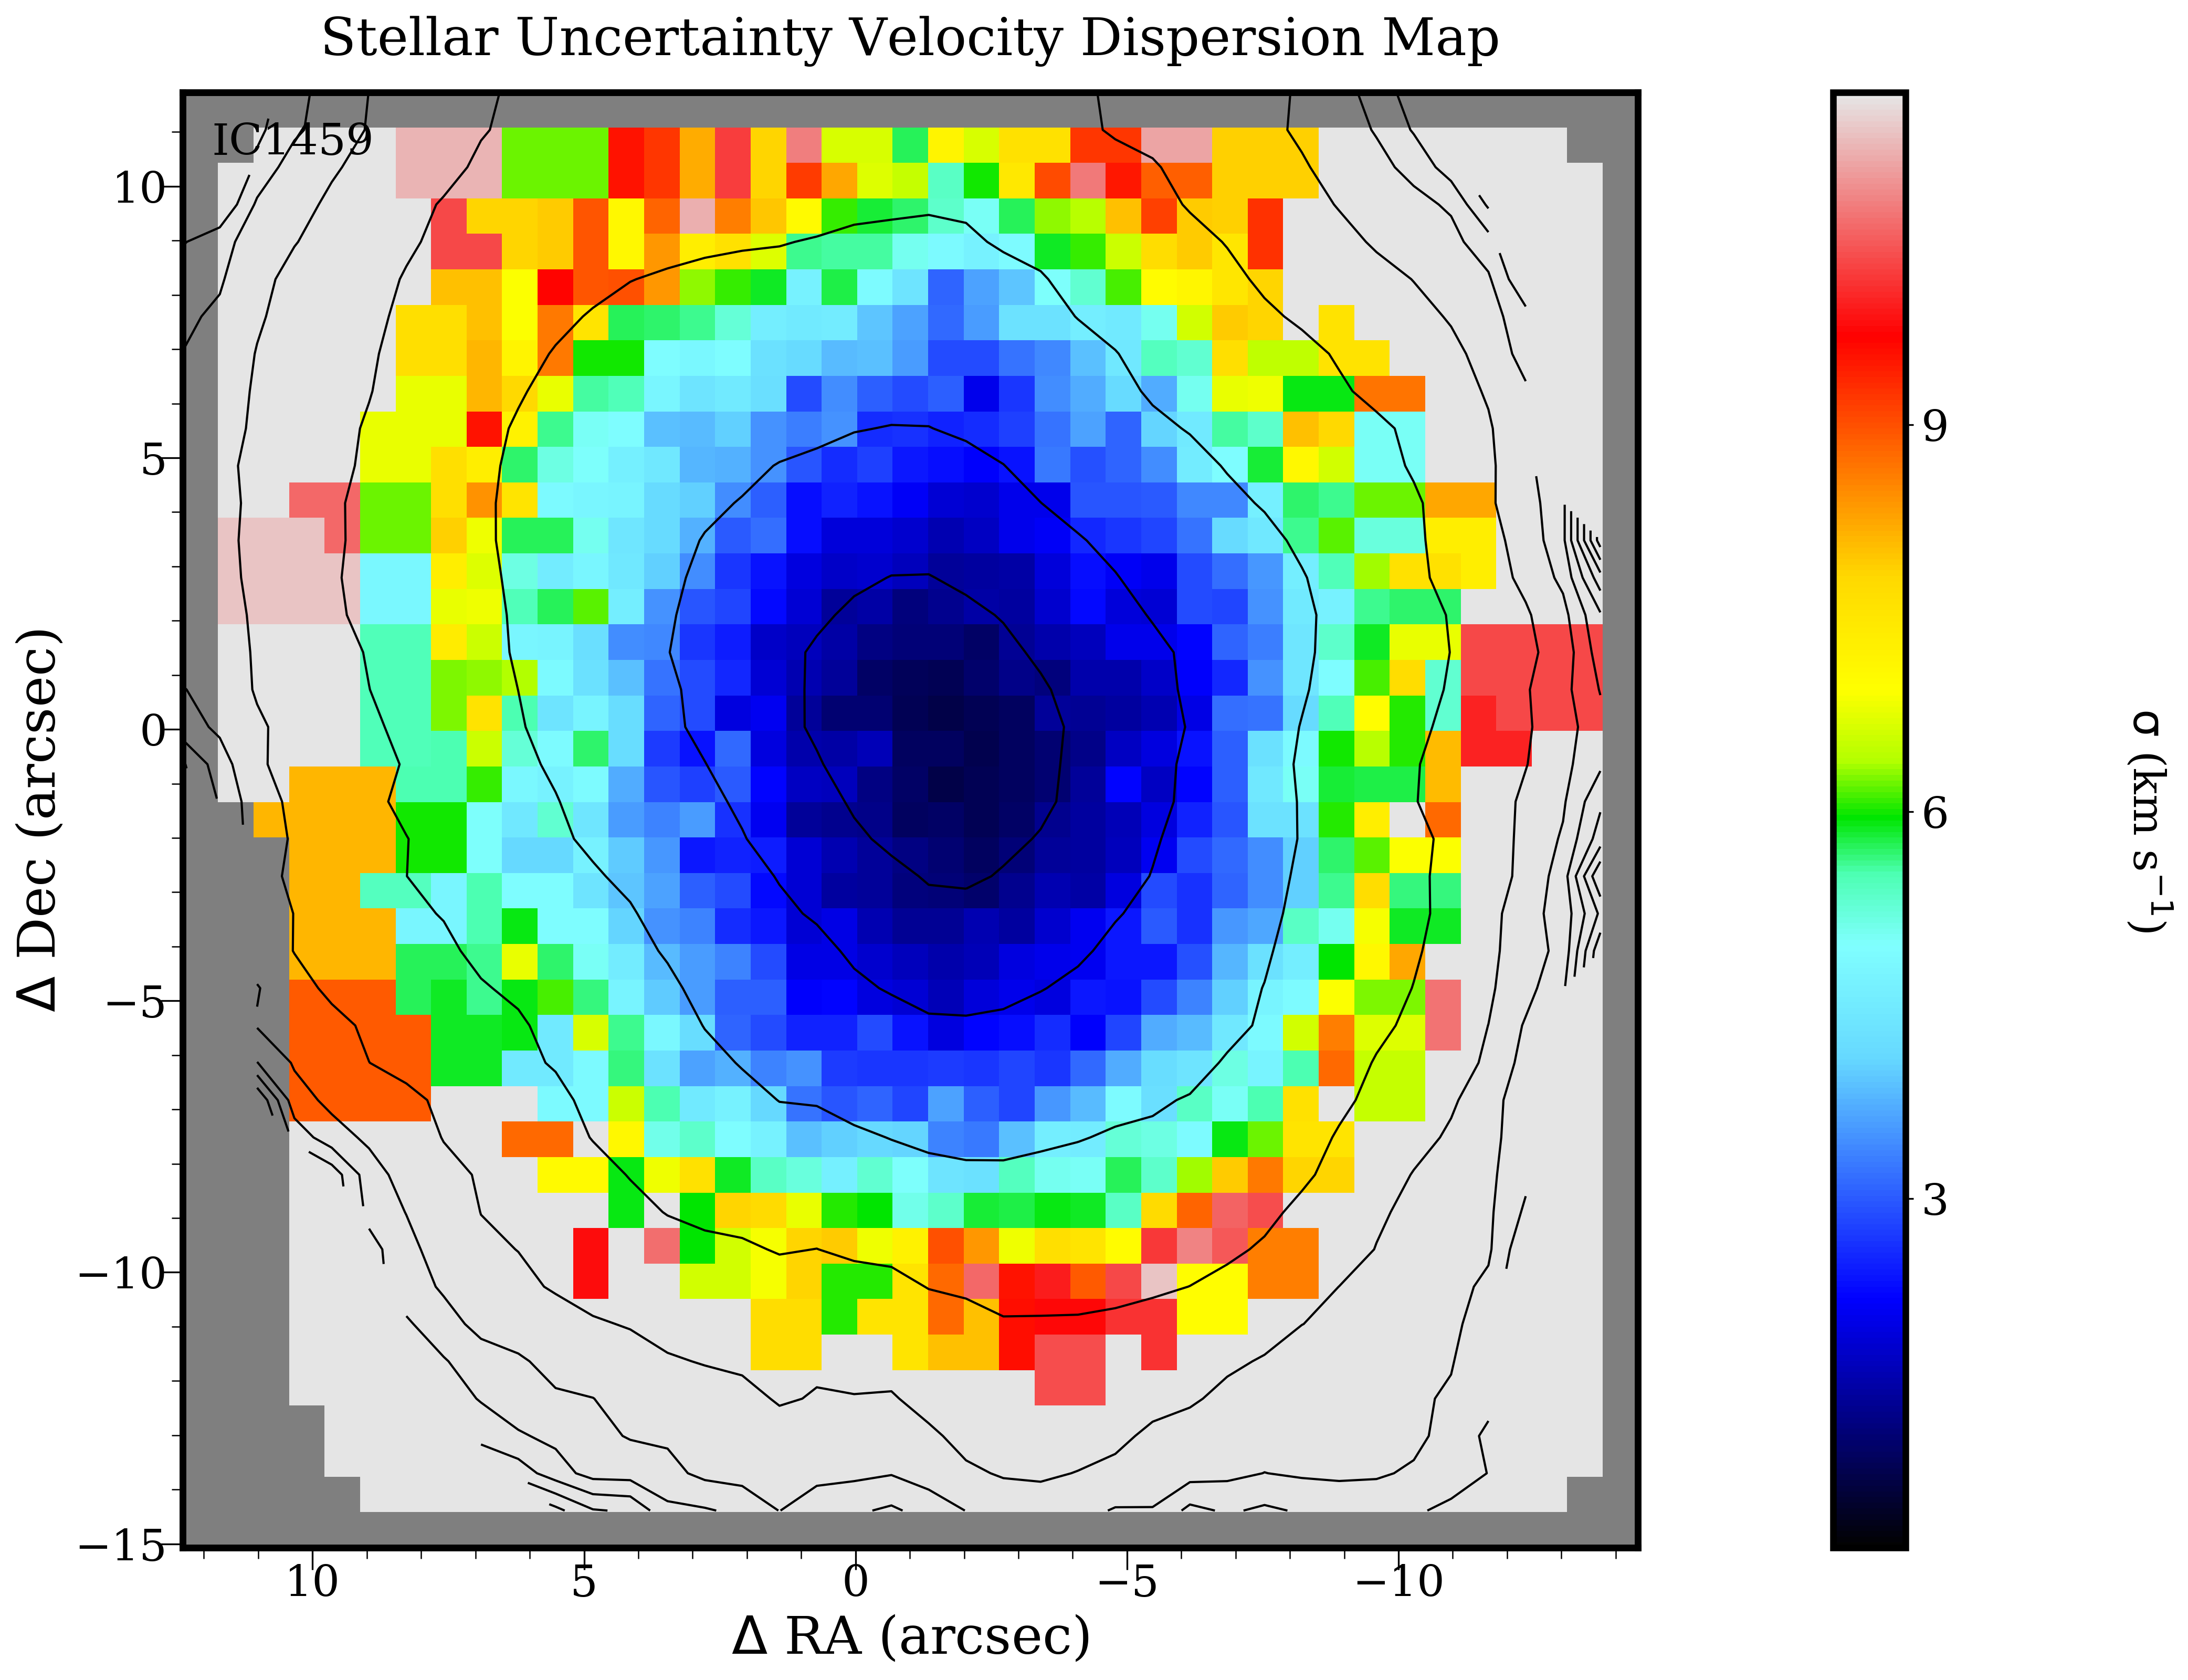
\includegraphics[width=0.245\textwidth]{Vmaps/ic1459_stellar_sigma_uncert.png}
      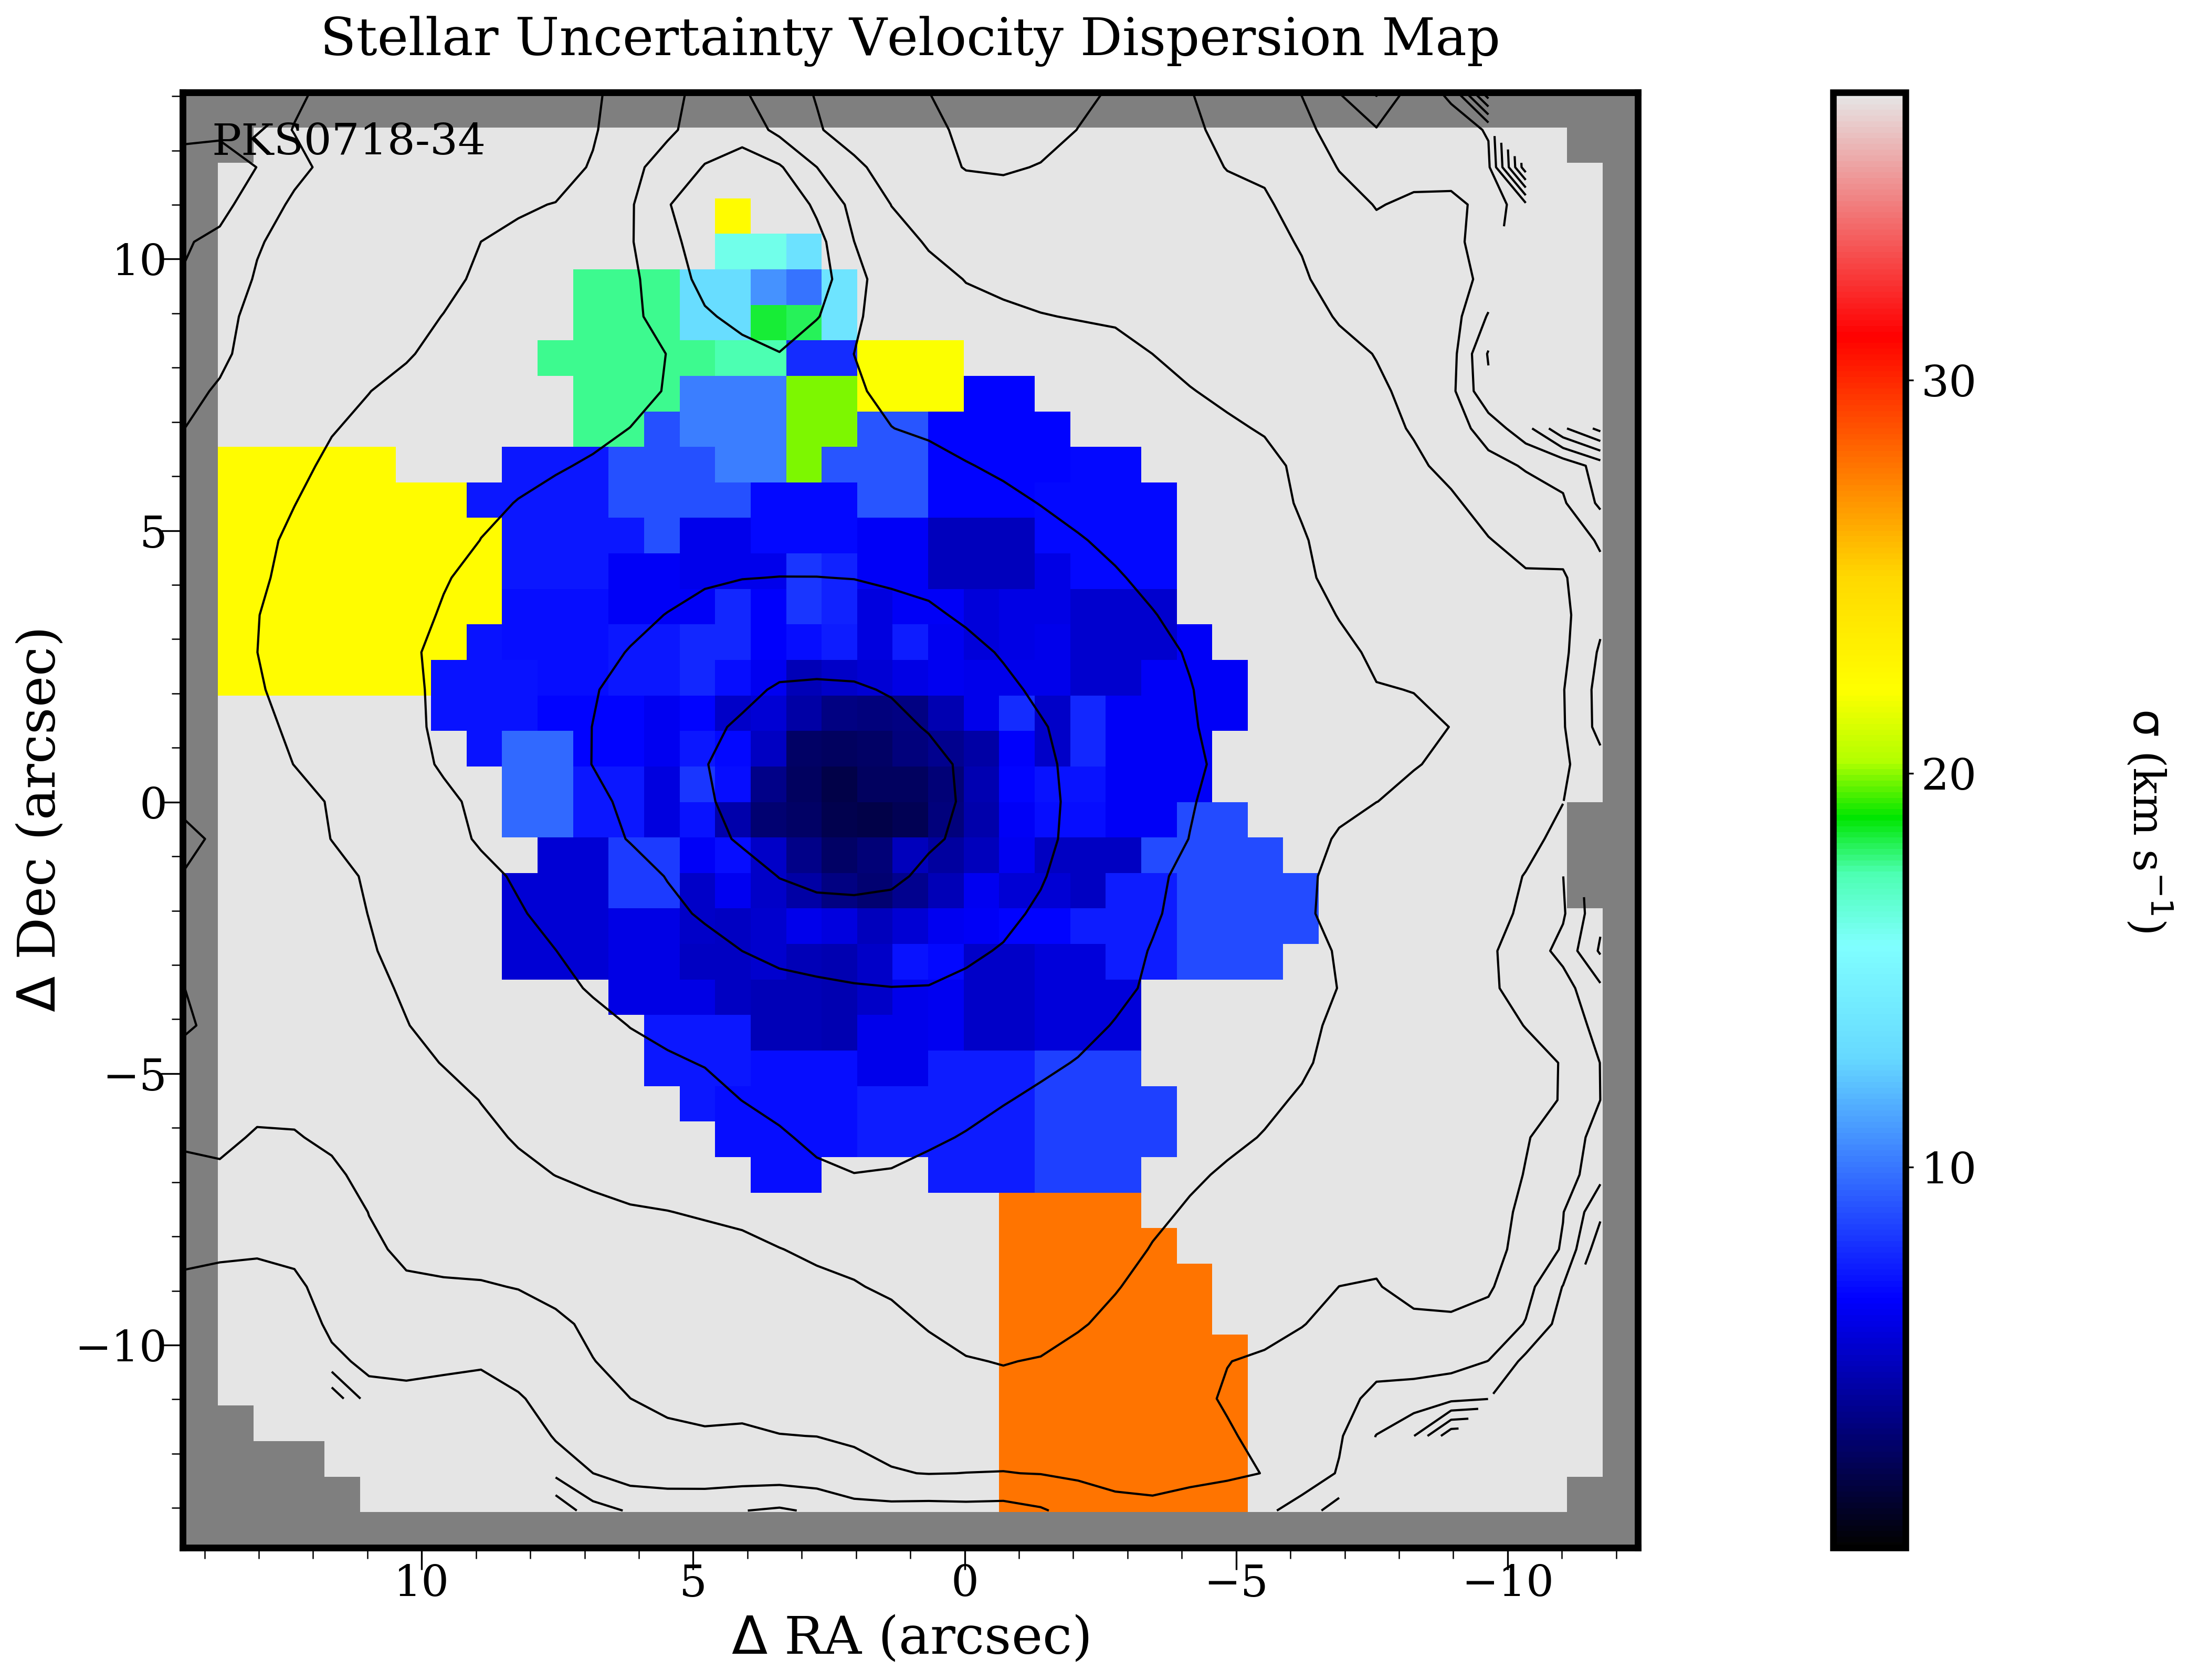
\includegraphics[width=0.245\textwidth]{Vmaps/pks0718-34_stellar_sigma_uncert.png}
      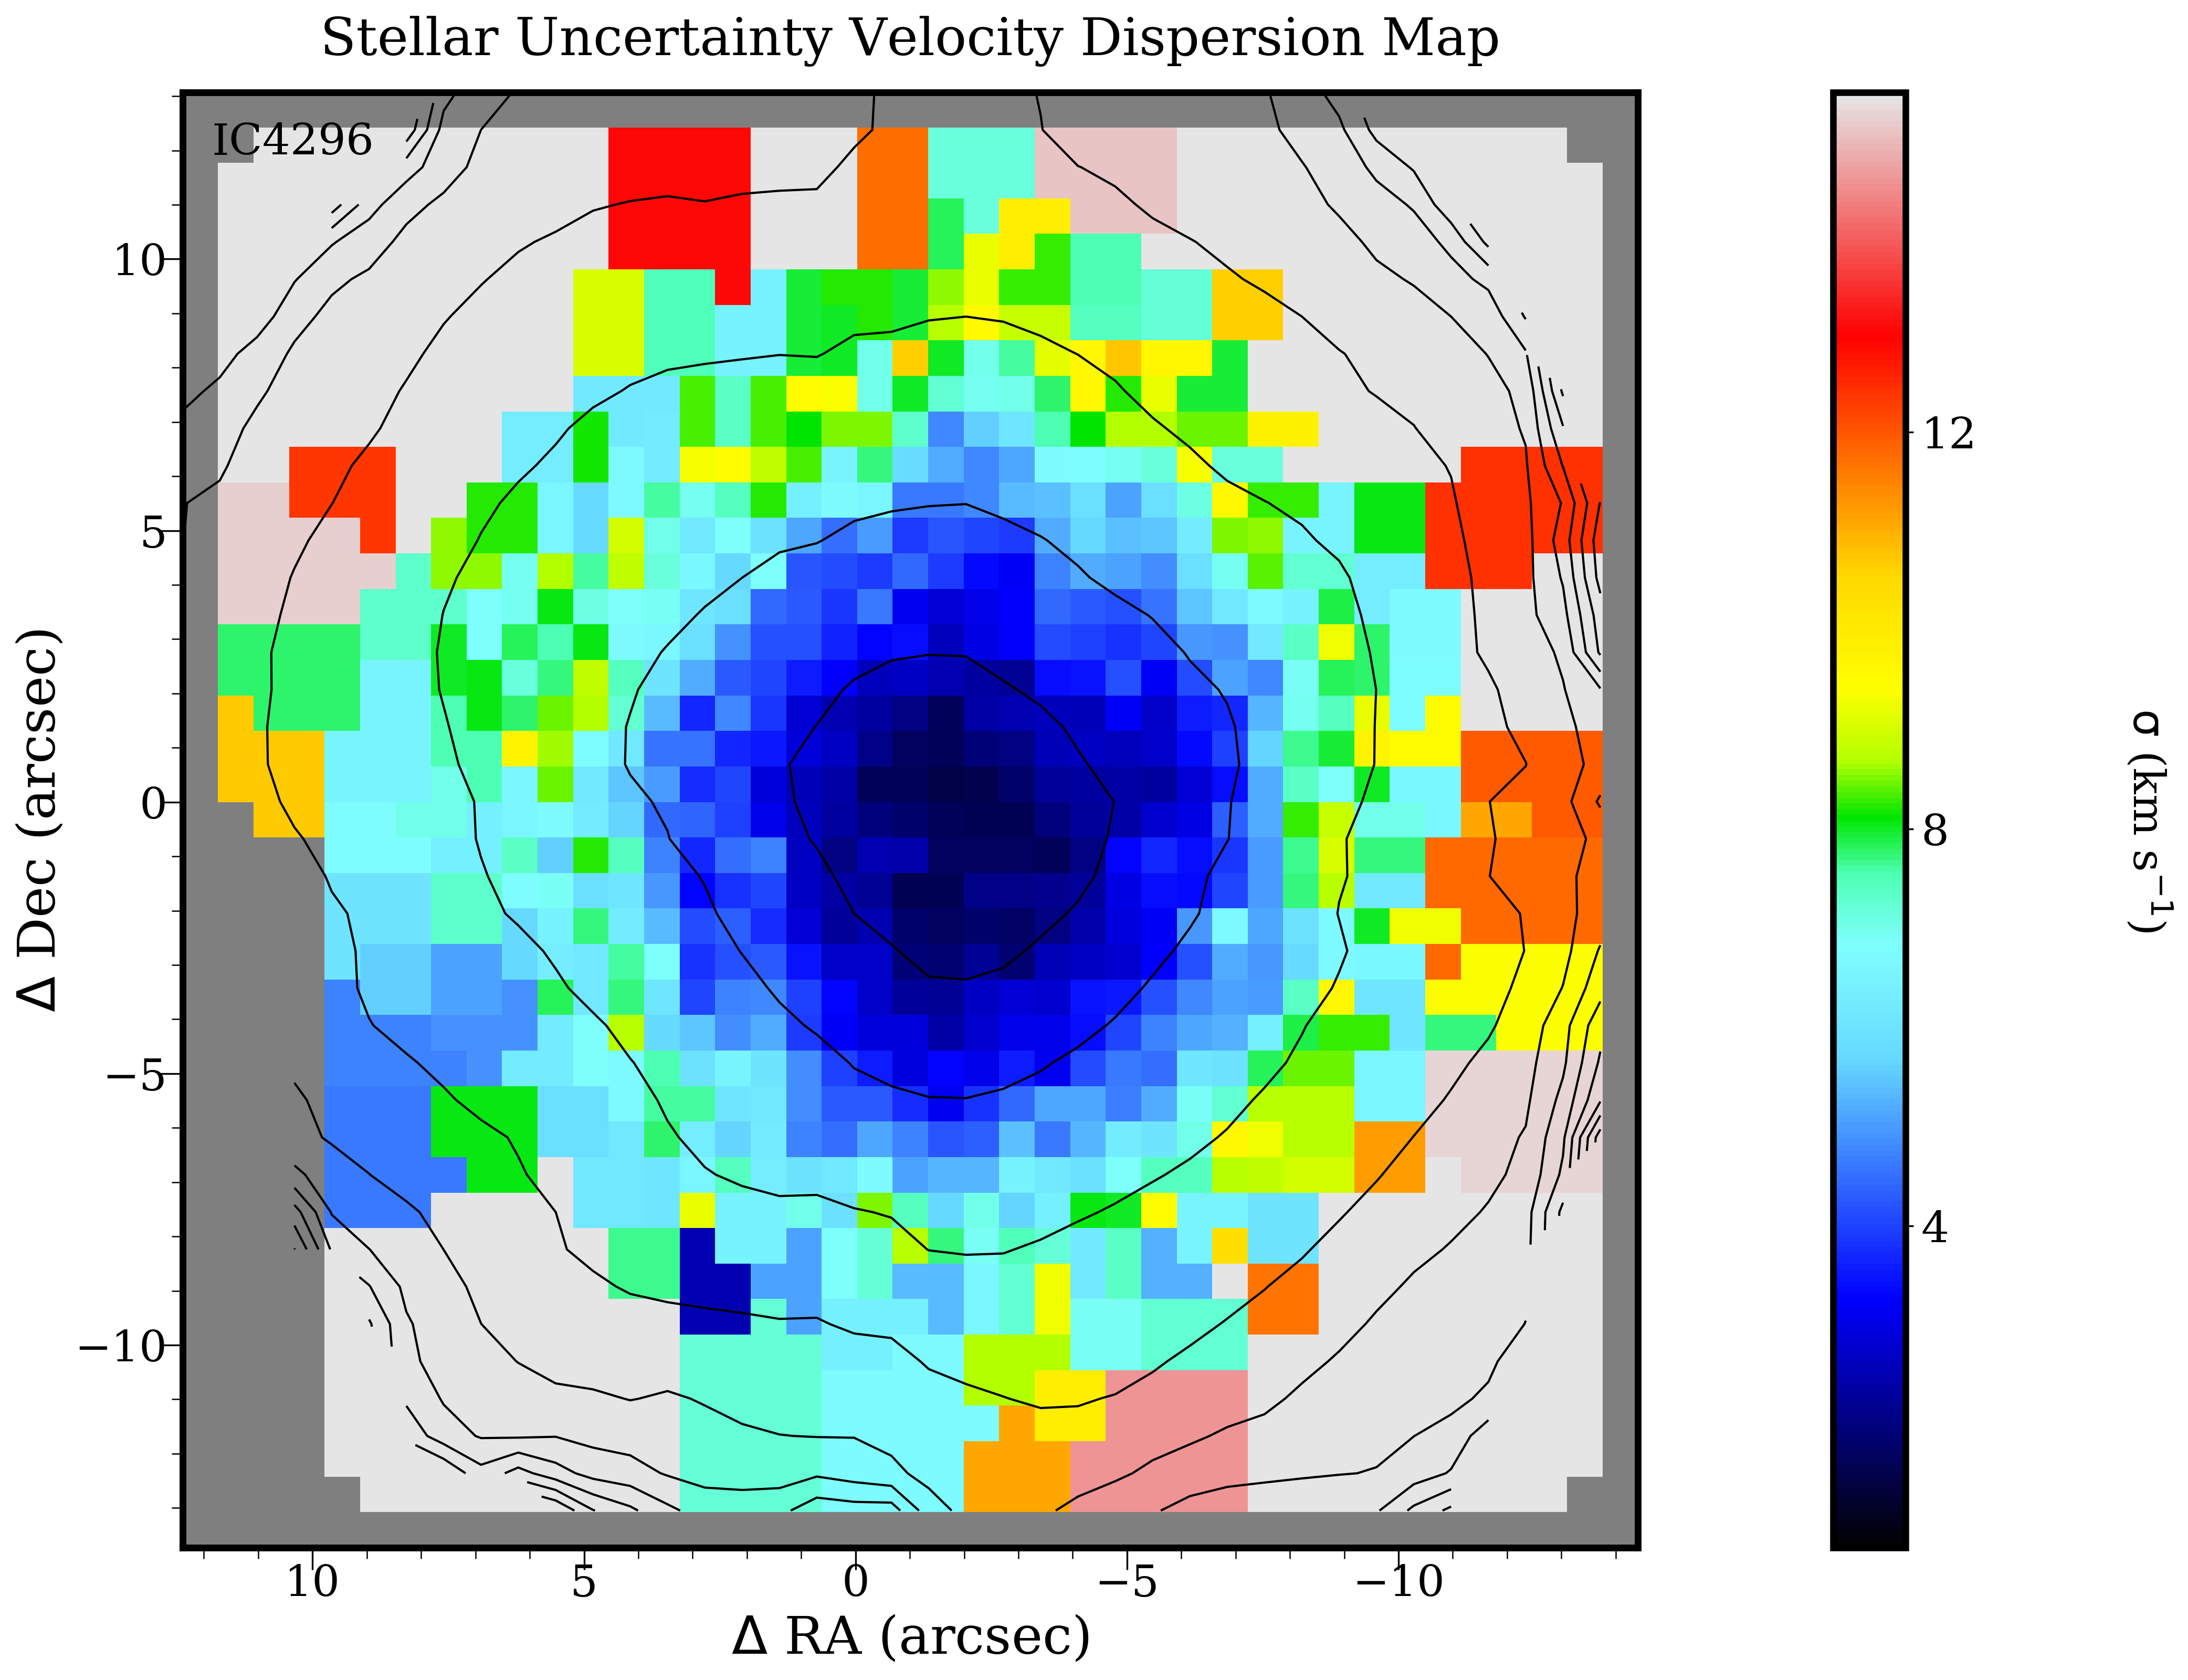
\includegraphics[width=0.245\textwidth]{Vmaps/ic4296_stellar_sigma_uncert.png}
      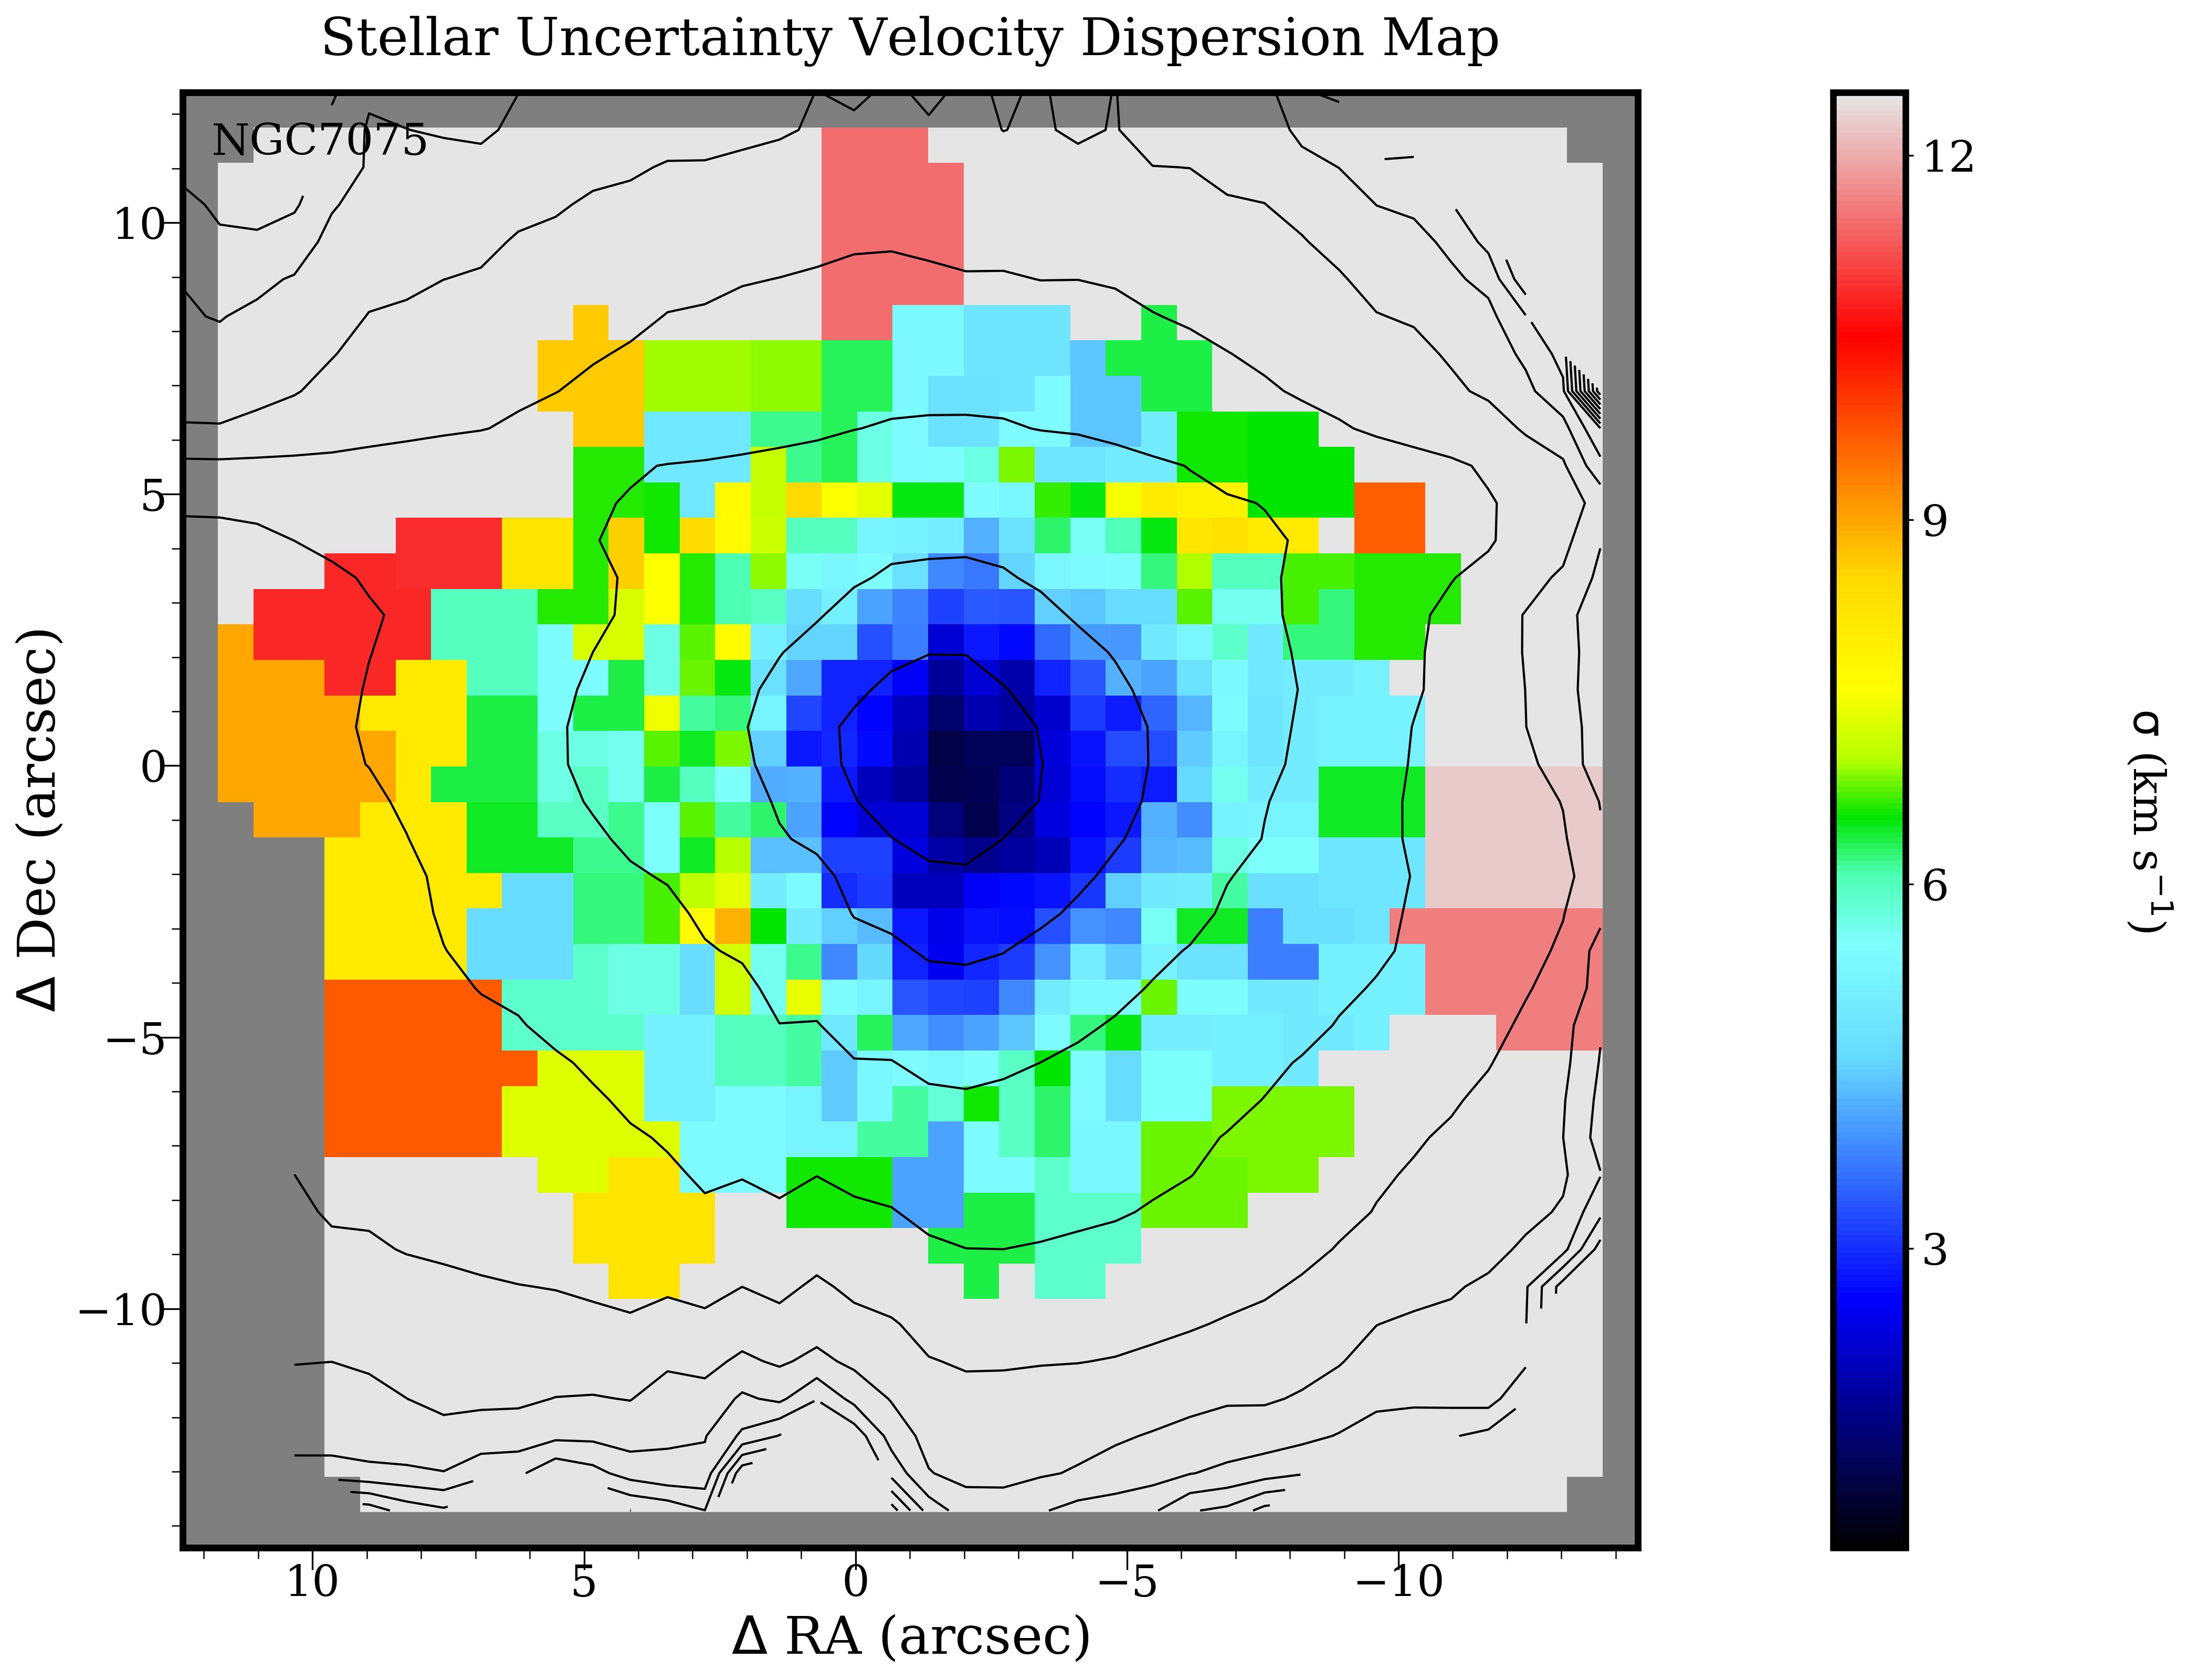
\includegraphics[width=0.245\textwidth]{Vmaps/ngc7075_stellar_sigma_uncert.png}
      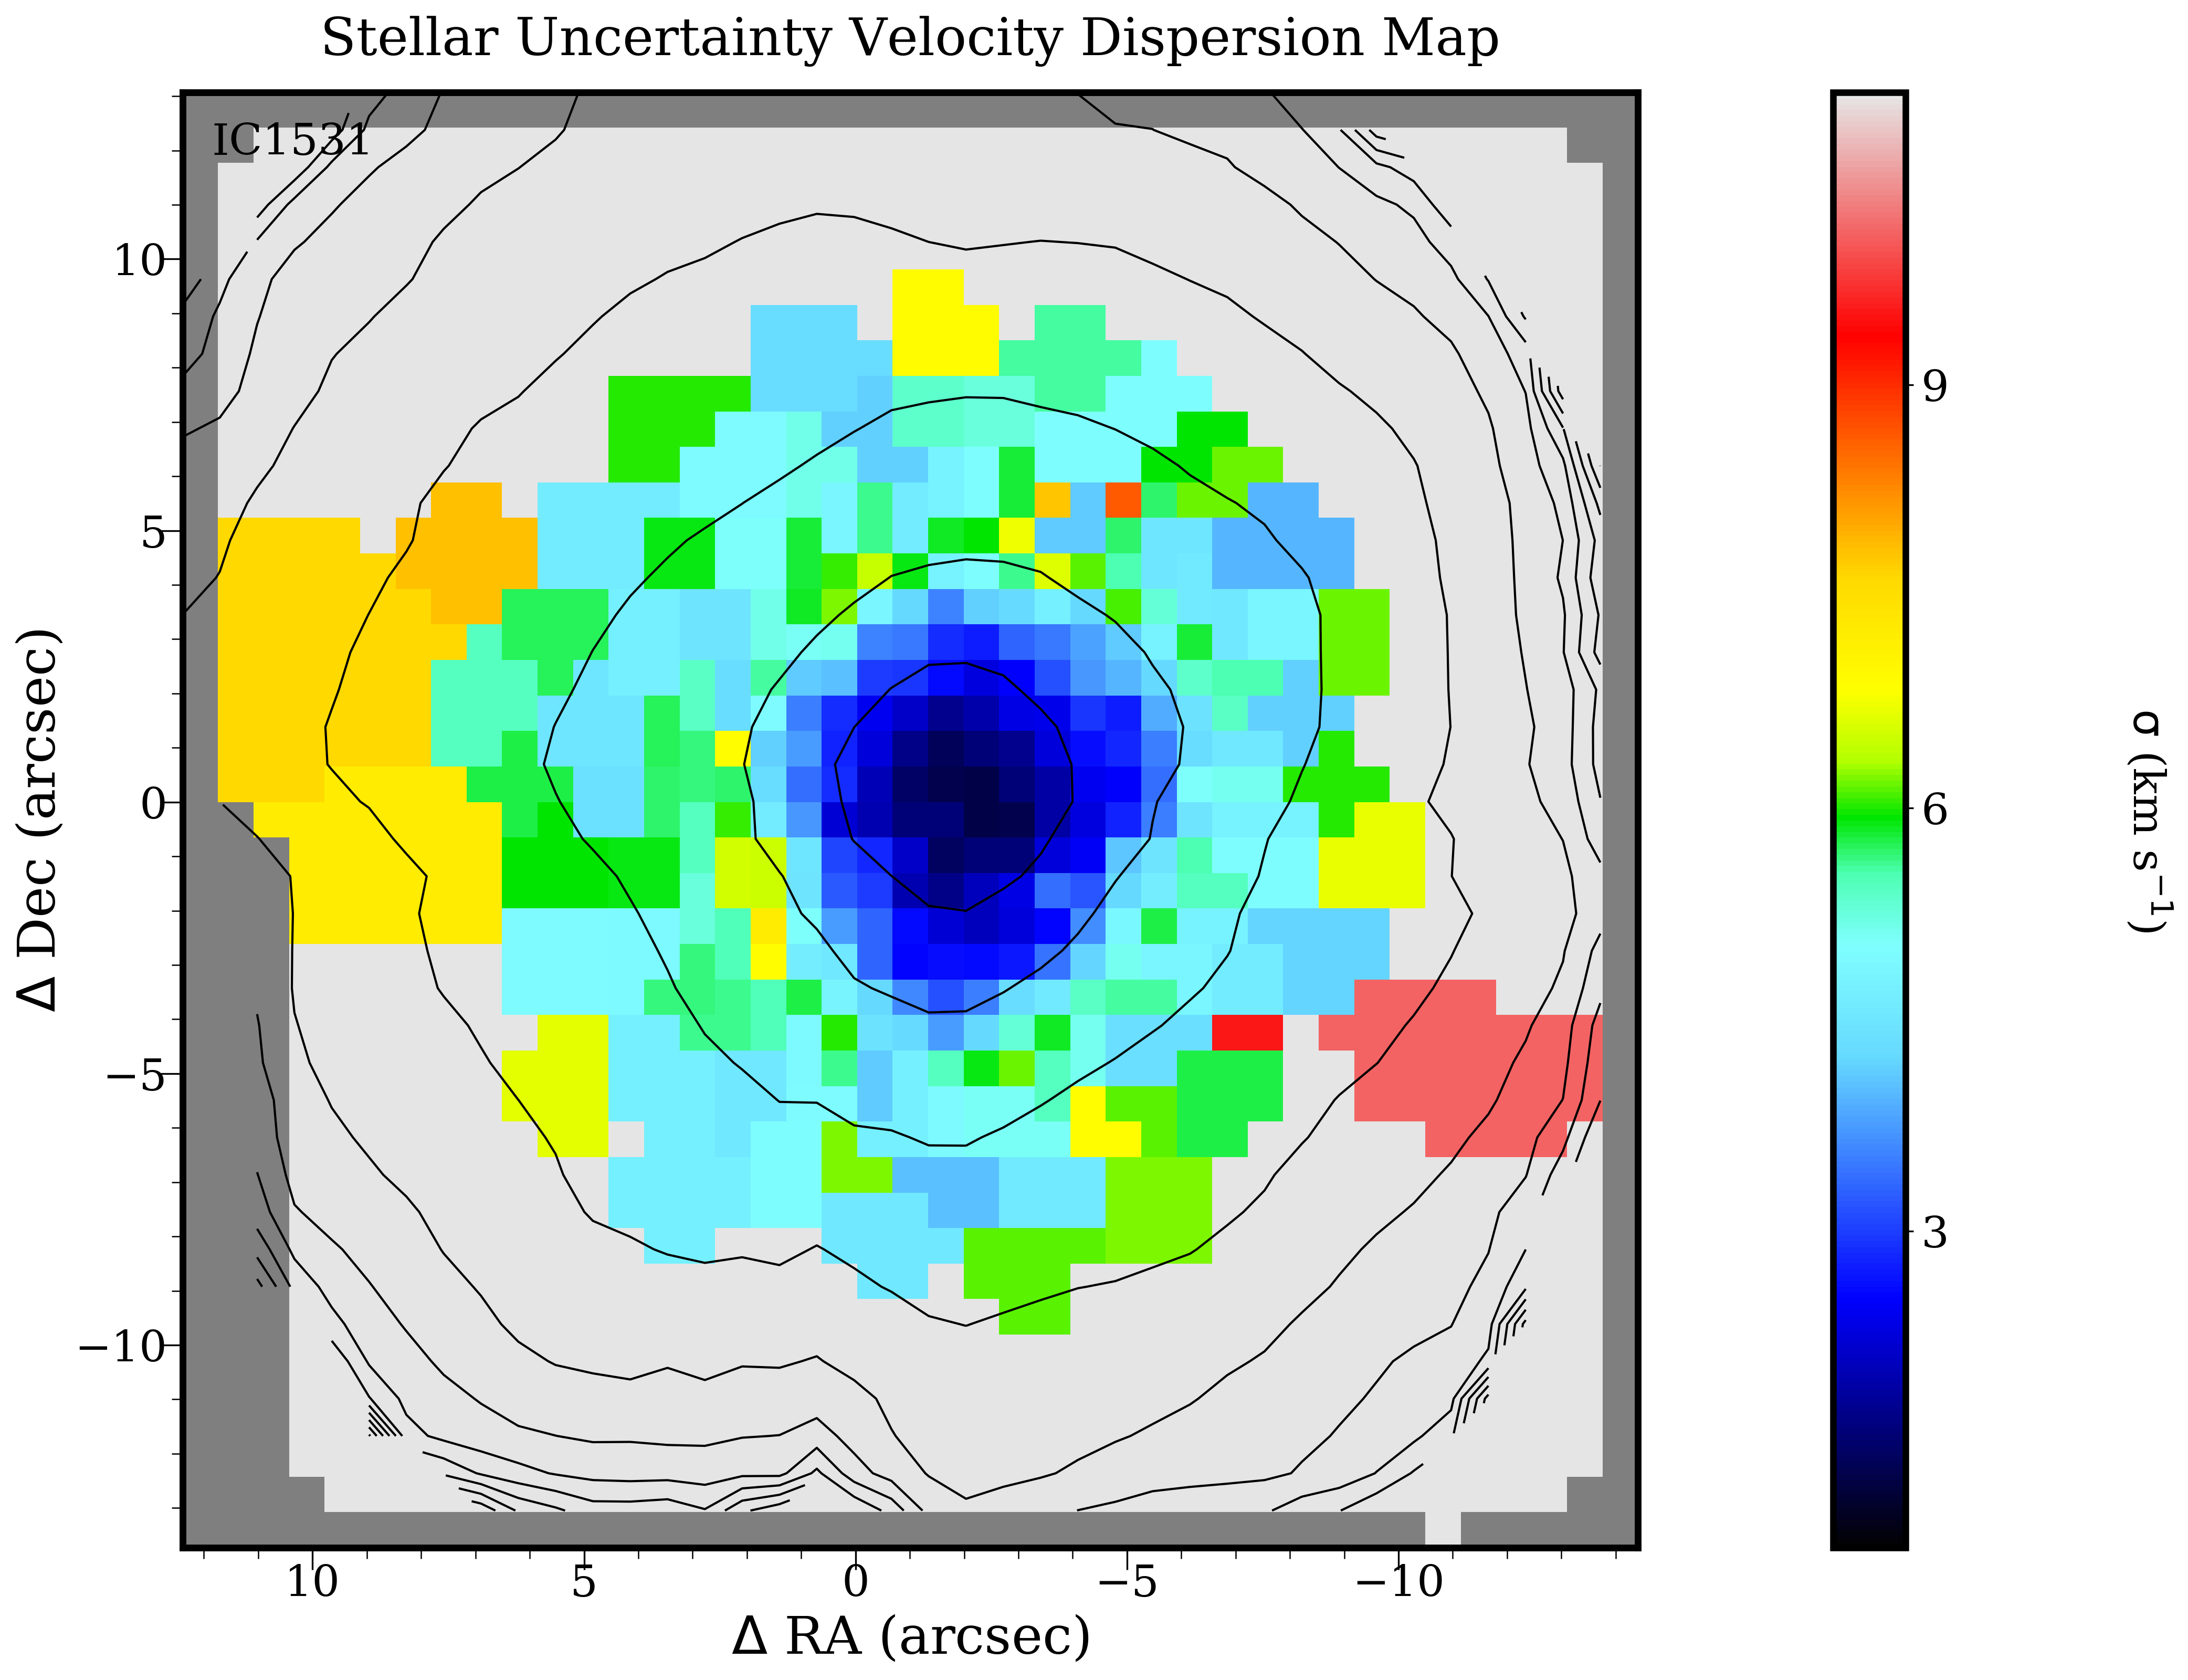
\includegraphics[width=0.245\textwidth]{Vmaps/ic1531_stellar_sigma_uncert.png}
      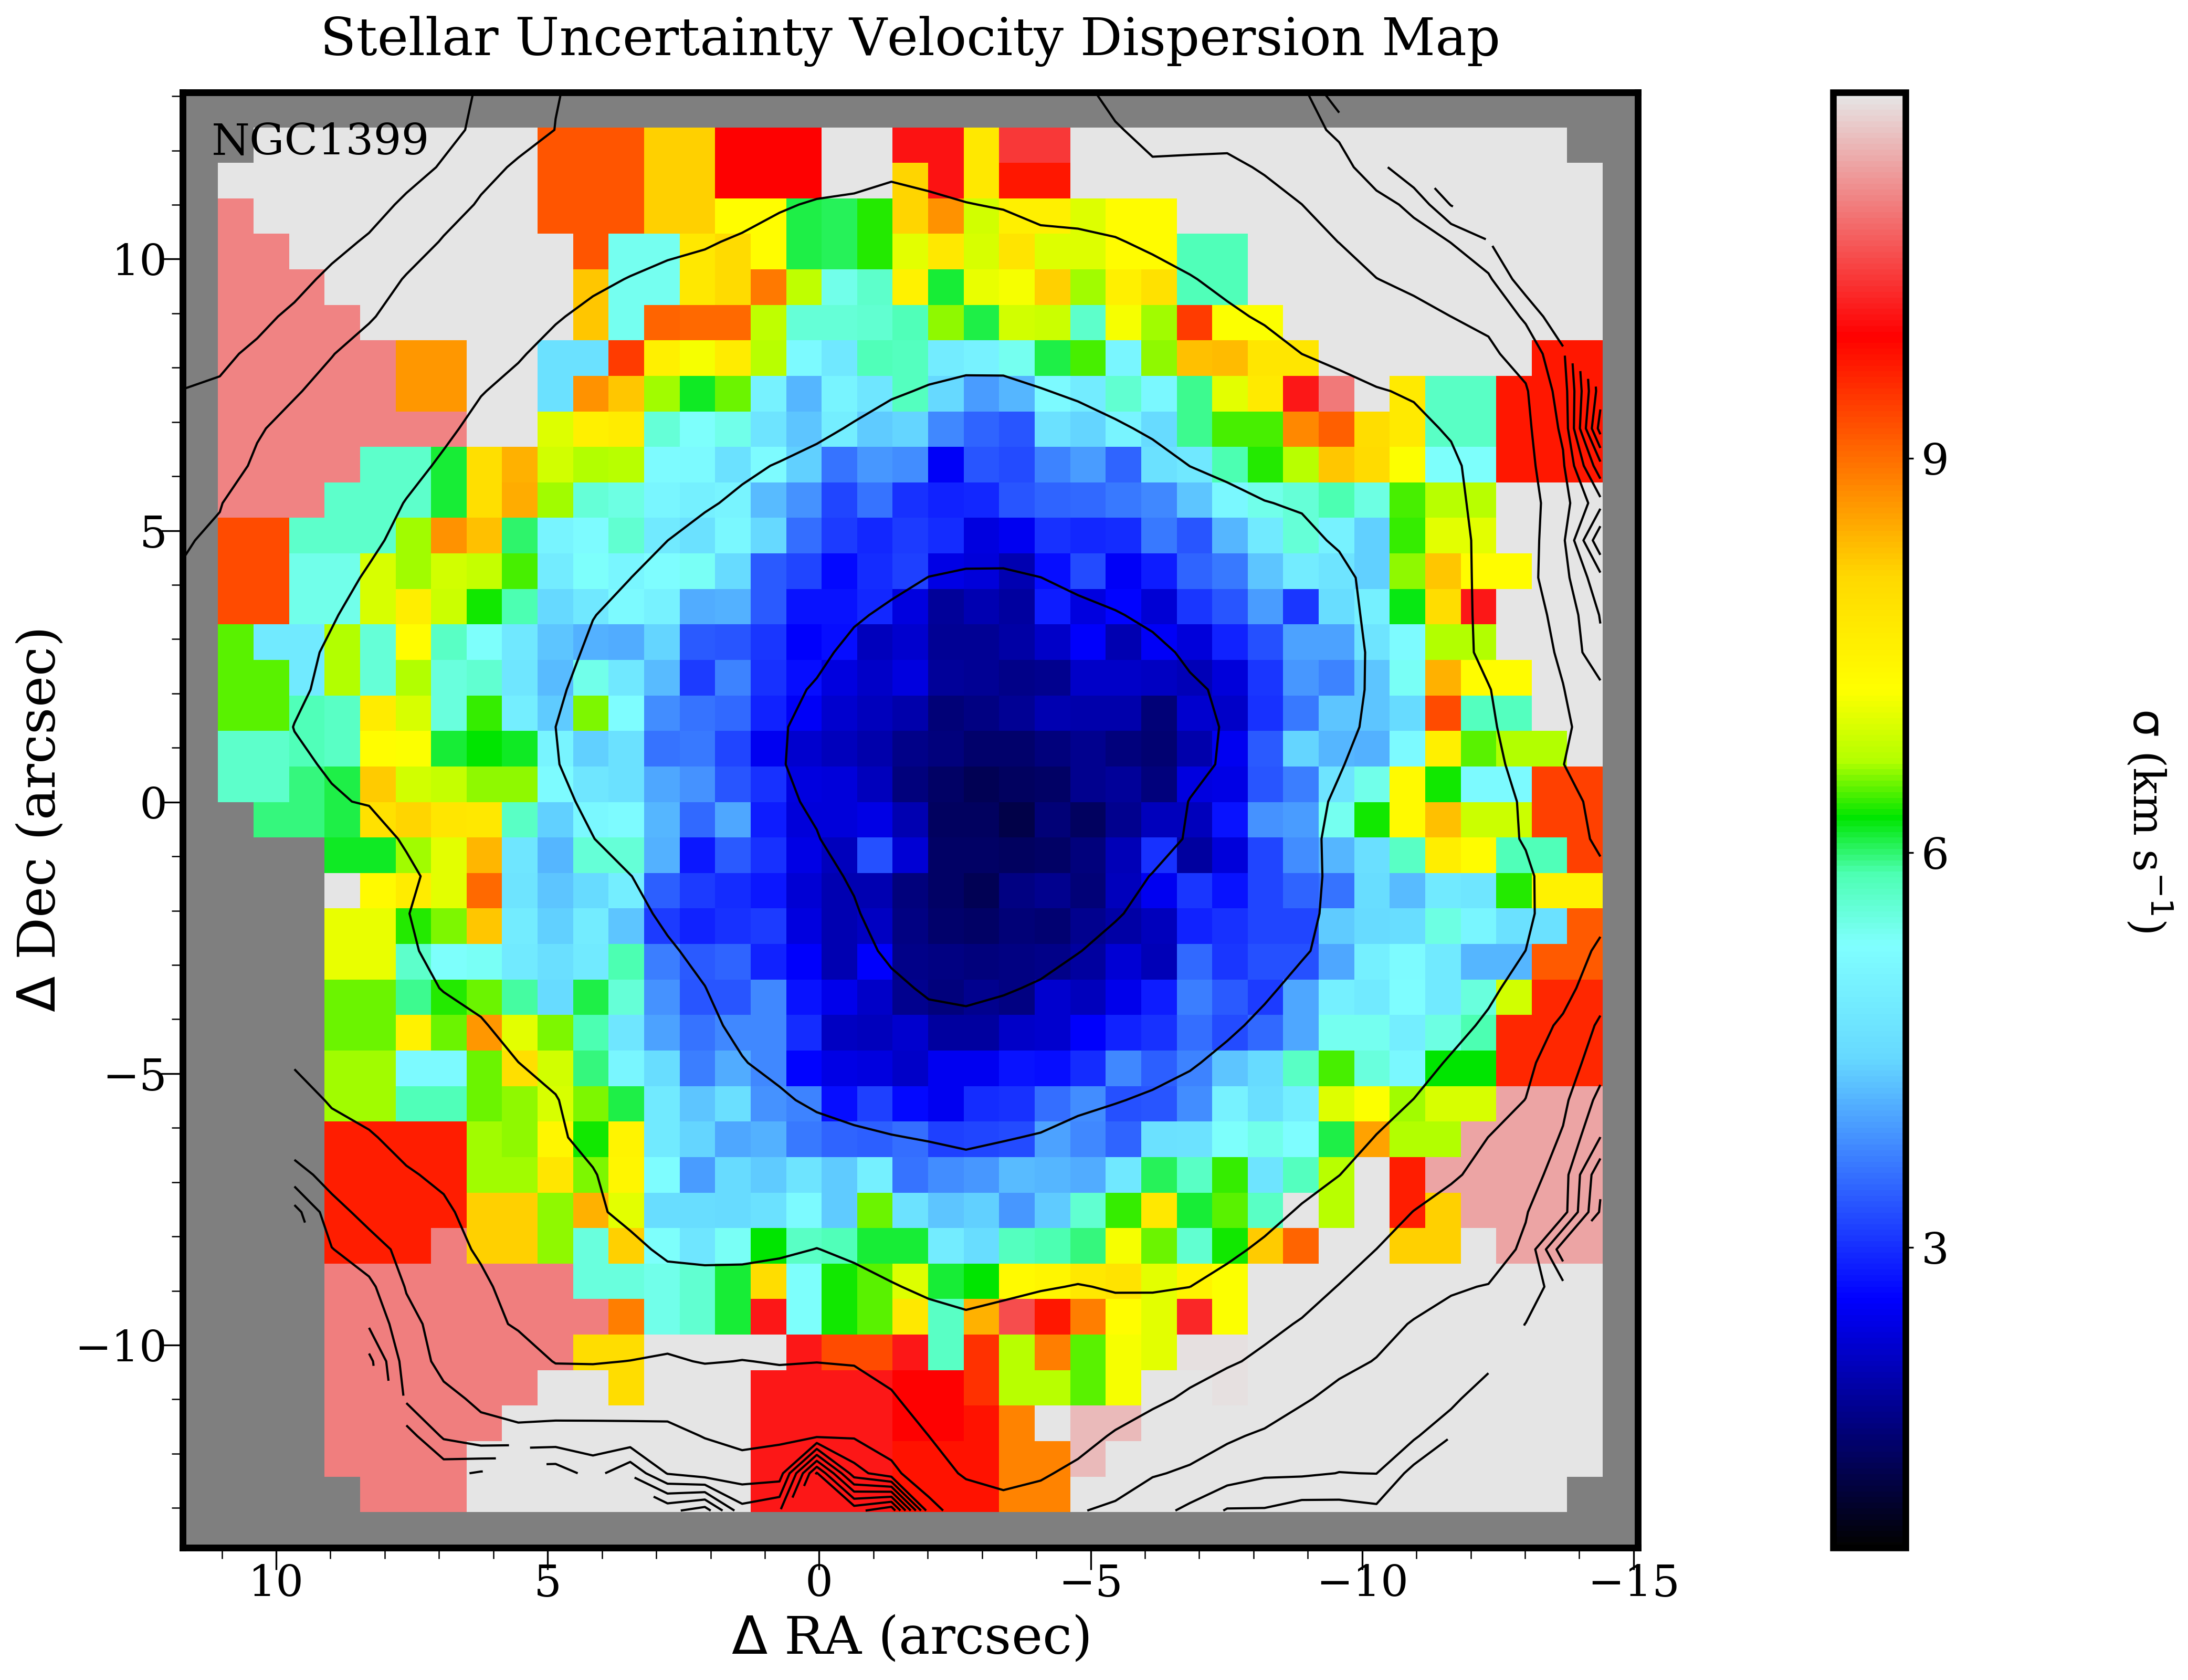
\includegraphics[width=0.245\textwidth]{Vmaps/ngc1399_stellar_sigma_uncert.png}
      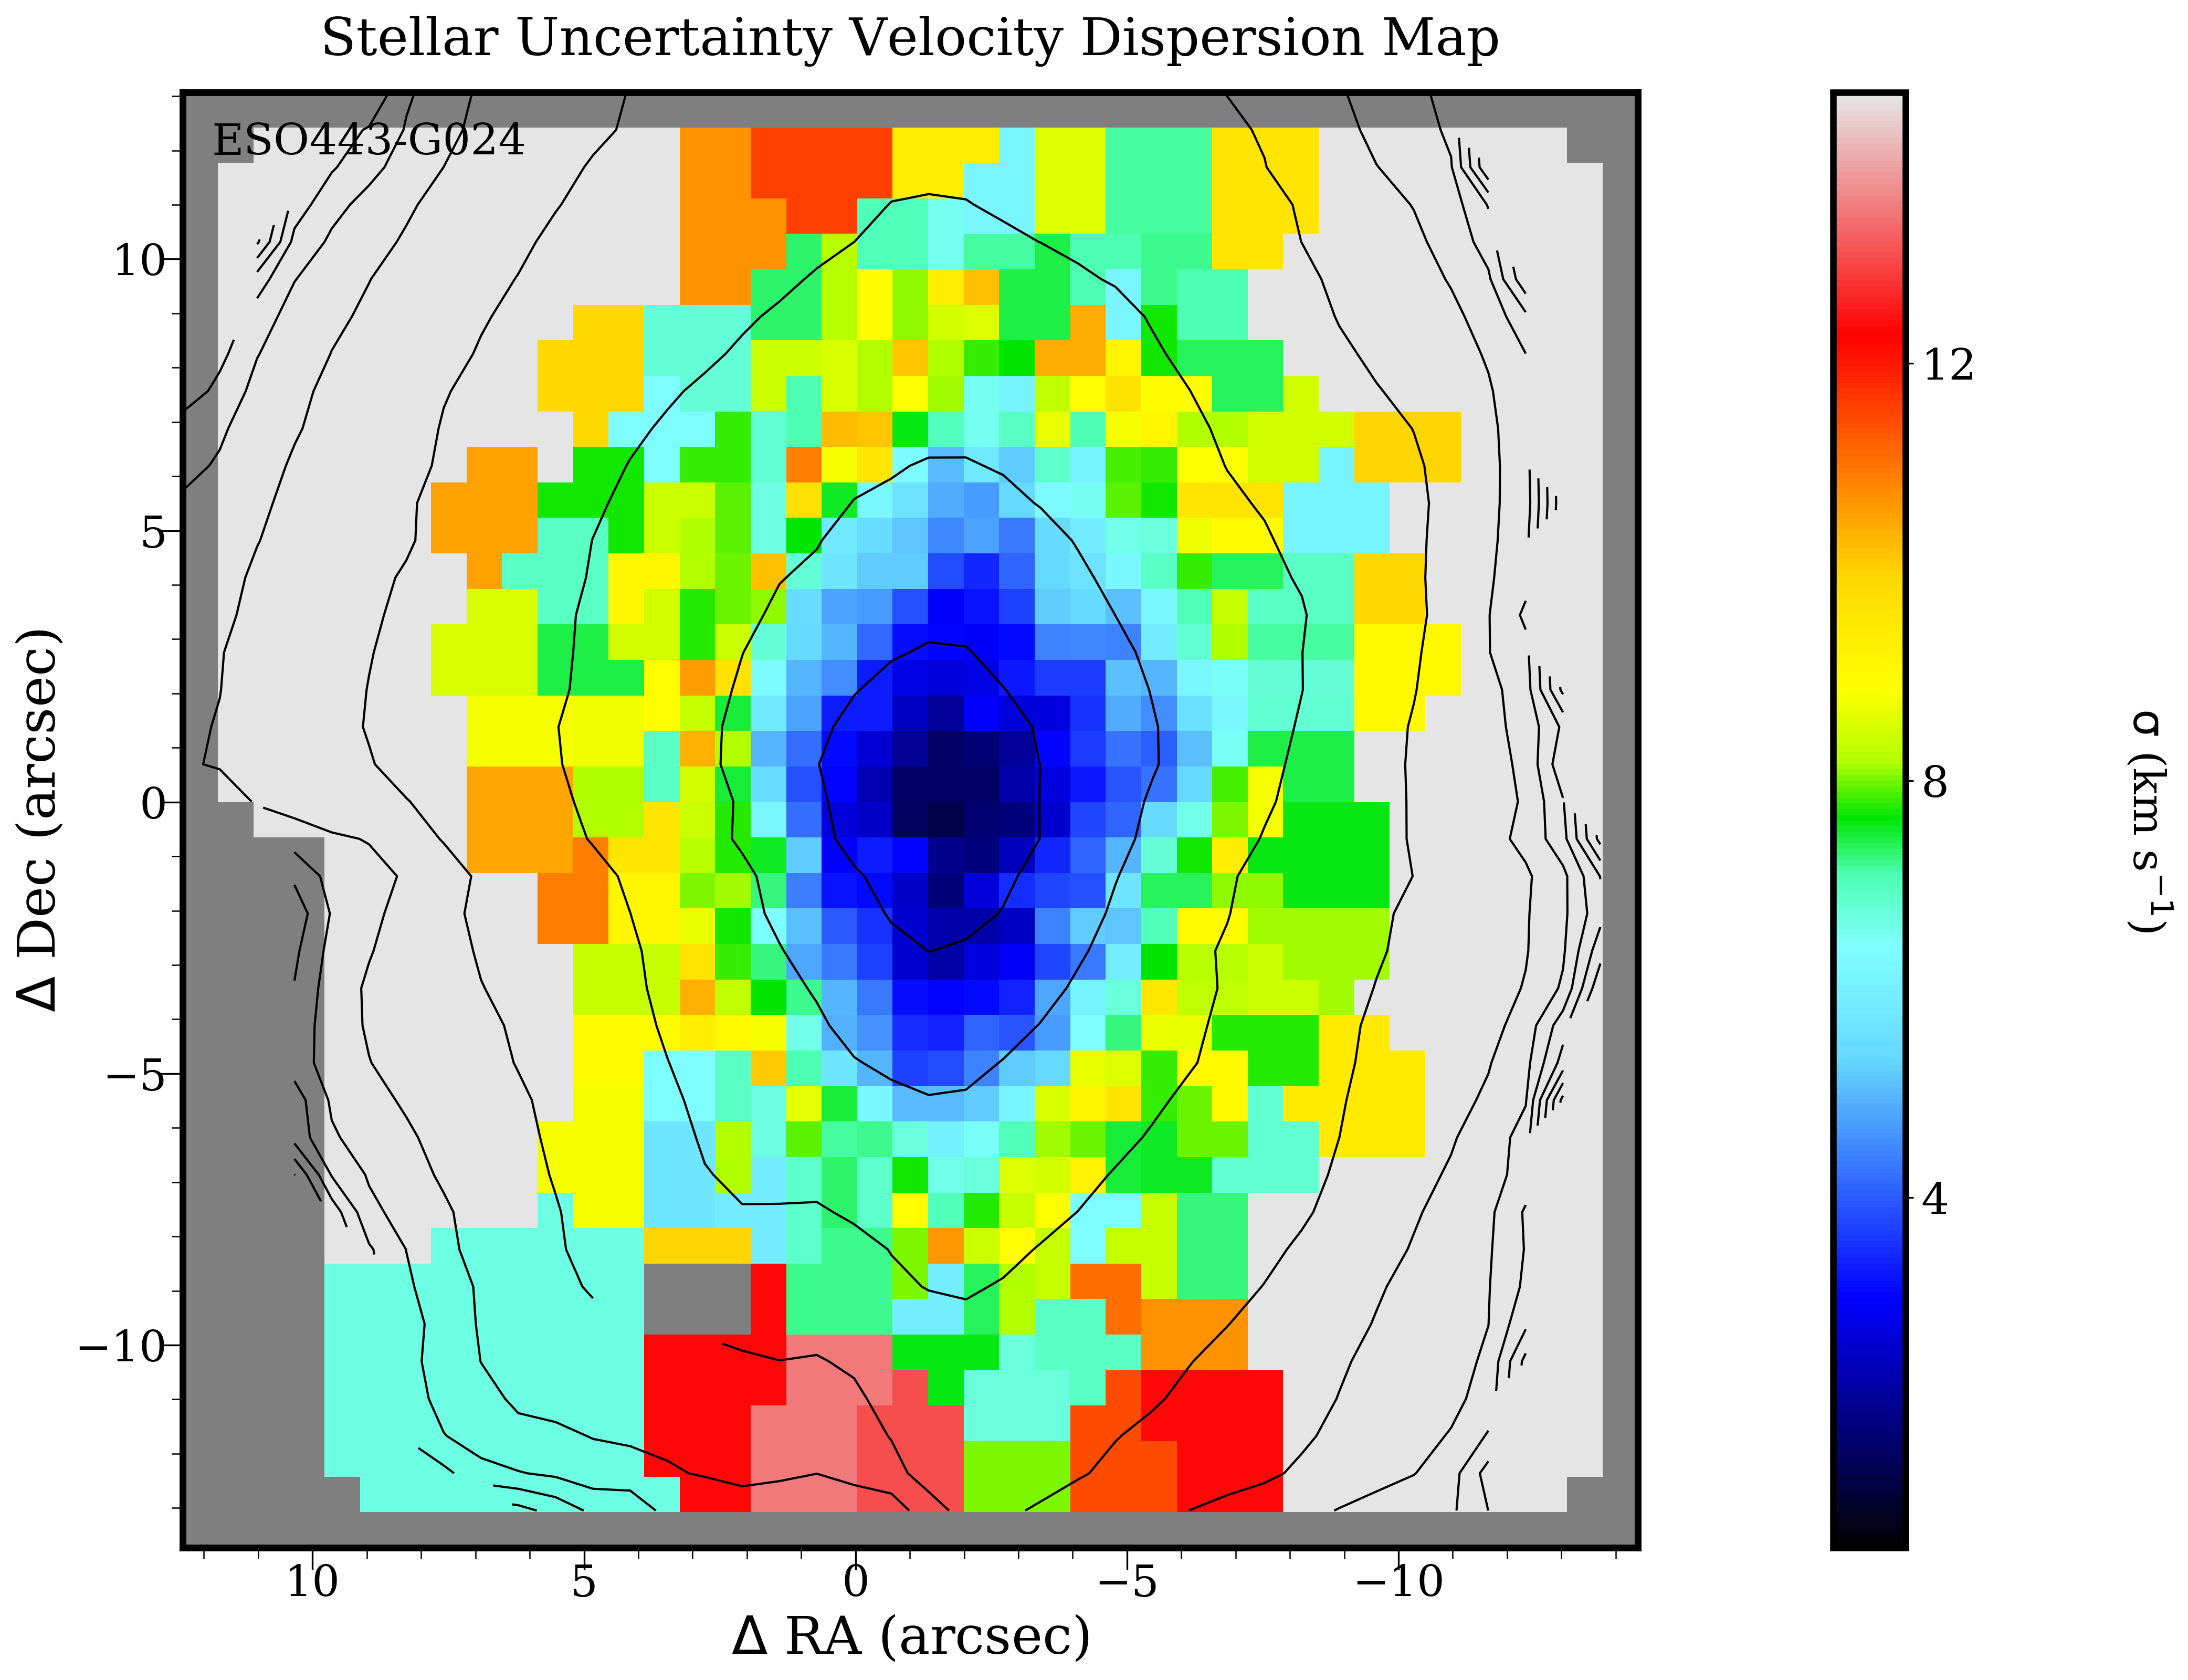
\includegraphics[width=0.245\textwidth]{Vmaps/eso443-g024_stellar_sigma_uncert.png}
      \caption[VIMOS dispersion uncertocity maps]{Uncertainties in the velocity dispersion for each galaxy in the VIMOS sample. Plots are ordered and contour colors are as in figure \ref{fig:Vstellar_img}}
      \label{fig:Vstellar_sigma_uncert}
\end{figure*}






\begin{figure*}
      \centering
      \includegraphics[width=0.245\textwidth]{Mmaps/ic1459_stellar_img.png}
      \includegraphics[width=0.245\textwidth]{Mmaps/ngc1316_stellar_img.png}
      \includegraphics[width=0.245\textwidth]{Mmaps/ic4296_stellar_img.png}
      \includegraphics[width=0.245\textwidth]{Mmaps/ngc1399_stellar_img.png}
      \caption[MUSE images]{Image for each galaxy in the MUSE sample. Plots are ordered roughly in peak stellar velocity with the contours as in figure \ref{fig:Vstellar_img}}
      \label{fig:Mstellar_img}
\end{figure*}

\begin{figure*}
      \centering
      \includegraphics[width=0.245\textwidth]{Mmaps/ic1459_stellar_vel.png}
      \includegraphics[width=0.245\textwidth]{Mmaps/ngc1316_stellar_vel.png}
      \includegraphics[width=0.245\textwidth]{Mmaps/ic4296_stellar_vel.png}
      \includegraphics[width=0.245\textwidth]{Mmaps/ngc1399_stellar_vel.png}
      \caption[MUSE velocity maps]{Velocity for each galaxy in the MUSE sample. Plots are ordered as in figure \ref{fig:Mstellar_img} and contour colors are as in figure \ref{fig:Vstellar_img}}
      \label{fig:stellar_vel}
\end{figure*}

\begin{figure*}
      \centering
      \includegraphics[width=0.245\textwidth]{Mmaps/ic1459_stellar_vel_uncert.png}
      \includegraphics[width=0.245\textwidth]{Mmaps/ngc1316_stellar_vel_uncert.png}
      \includegraphics[width=0.245\textwidth]{Mmaps/ic4296_stellar_vel_uncert.png}
      \includegraphics[width=0.245\textwidth]{Mmaps/ngc1399_stellar_vel_uncert.png}
      \caption[MUSE velocity uncertocity maps]{Uncertainties in the velocity for each galaxy in the MUSE sample. Plots are ordered as in figure \ref{fig:Mstellar_img} and contour colors are as in figure \ref{fig:Vstellar_img}}
      \label{fig:Mstellar_vel_uncert}
\end{figure*}

\begin{figure*}
      \centering
      \includegraphics[width=0.245\textwidth]{Mmaps/ic1459_stellar_sigma.png}
      \includegraphics[width=0.245\textwidth]{Mmaps/ngc1316_stellar_sigma.png}
      \includegraphics[width=0.245\textwidth]{Mmaps/ic4296_stellar_sigma.png}
      \includegraphics[width=0.245\textwidth]{Mmaps/ngc1399_stellar_sigma.png}
      \caption[MUSE velocity dispersion]{Velocity dispersion for each galaxy in the MUSE sample. Plots are ordered as in figure \ref{fig:Mstellar_img} and contour colors are as in figure \ref{fig:Vstellar_img}}
      \label{fig:Mstellar_sigma}
\end{figure*}


\begin{figure*}
      \centering
      \includegraphics[width=0.245\textwidth]{Mmaps/ic1459_stellar_sigma_uncert.png}
      \includegraphics[width=0.245\textwidth]{Mmaps/ngc1316_stellar_sigma_uncert.png}
      \includegraphics[width=0.245\textwidth]{Mmaps/ic4296_stellar_sigma_uncert.png}
      \includegraphics[width=0.245\textwidth]{Mmaps/ngc1399_stellar_sigma_uncert.png}
      \caption[MUSE dispersion uncertocity maps]{Uncertainties in the velocity dispersion for each galaxy in the MUSE sample. Plots are ordered as in figure \ref{fig:Mstellar_img} and contour colors are as in figure \ref{fig:Vstellar_img}}
      \label{fig:Mstellar_sigma_uncert}
\end{figure*}

		Figures \ref{fig:Vstellar_img} - \ref{fig:Mstellar_sigma_uncert} show the stellar LOSVD with associated uncertainties for all VIMOS and MUSE datacubes. 

		The kinematics of the sample are classified according to the Regular-Rotator/Non Regular-Rotator (RR/NRR) regime given in \citet{Krajnovic2011}, Fast/Slow Rotator (FR/SR) regime given in \citet{Cappellari2016} (originally defined by \citet{Emsellem2011}, but later refined by \citet{Cappellari2016}). This classification is shown on the $\lambda_{R_e}$--ellipticity plane in figure \ref{fig:lambdaR_ellip}. Beyond this attempts have been made to use the kinematic features as defined in \citet{Krajnovic2011}, however the quality of the data has meant that many have had to be classified by eye as the artifacts from the VIMOS quadrants confuse any ellipse fitting methods. For VIMOS maps, the classifications are done by eye. These classifications are given in table \ref{tab:classify}. 


		\begin{table}
			\centering
			\caption{Kinematic classifications. Where we have MUSE datacubes, the value and classifications from this are given (since they rely on less extrapolation due to the larger field of view of MUSE), otherwise the values are from the VIMOS maps. Col. 1: Galaxy name, Col. 2: $\lambda_{R_e}$, Col. 3: ellipticity, Col. 4: Misalignment between kinematic position angle and photometric position angle, Col. 5: Fast or Slow rotator, Col. 6: Regular rotator or non-regular rotator, Col. 7: Kinematic features (abbreviations defined in section \ref{sec:ETG}), Col. 8: Kinematic group as defined in section \ref{sec:ETG}}
			\label{tab:classify}
			\begin{tabular}{l r r p{0.7cm} p{0.8cm} p{0.8cm} p{1cm} p{1cm}}
				\hline
				\hline
				Galaxy		& $\lambda_{R_e} & $\epsilon$  & $\Gamma_\text{kin}$ (deg) & FR/ SR 	& RR/ NRR 	& Feat. & Group 	\\
				\hline 
				ESO 443-G024 & 0.031 & 0.32 & 55.3 & FR & NRR & KDC & c \\
				IC 1459 	& 0.174 & 0.24 & 5.1 & FR & NRR & KDC & c \\
				IC 1531 	& 0.100 & 0.11 & 115.5 & SR & NRR & LV & a \\
				IC 4296		& 0.034 & 0.03 & \_\_\_\_ & SR & NRR & KDC & c \\
				NGC 612 	& 0.519 & 0.58 & \_\_\_\_ & FR & RR & -- & e \\
				NGC 1316 	& 0.100 & 0.39 & \_\_\_\_ & SR & NRR & -- & f \\
				NGC 1399 	& 0.090 & 0.12 & \_\_\_\_ & SR & NRR & LV & a \\
				NGC 3100 	& 0.418 & 0.31 & \_\_\_\_ & FR & RR & -- & e \\
				NGC 3557 	& 0.320 & 0.22 & \_\_\_\_ & FR & RR & -- & e\\
				NGC 7075 	& 0.048 & 0.09 & \_\_\_\_ & SR & NRR & -- & b \\
				PKS 0718-34 & 0.152 & 0.18 & \_\_\_\_ & SR & NRR & KDC? & b\\
				\hline
				\hline
			\end{tabular}
		\end{table}


		\begin{figure}
			\centering
			\includegraphics[width=\textwidth]{chapter4/lambdaR_ellipticity.png}
			\caption[$\lambda_{R_e}$ -- ellipticity plane]{The $\lambda_{R_e}$ -- ellipticity plane showing the definition for the fast/slow rotator classes (solid black line). Atlas3D galaxies are shown in black \citep{Emsellem2011} and MASSIVE survey galaxies are shown in grey \citep{Veale2017}. The theoretic limit of disk dominated galaxy is shown (solid magenta) with lines of constant intrinsic angular moment with varying inclination (dashed magenta). VIMOS and MUSE measurements are shown in red and blue respectively. Note: the MASSIVE survey does not classify substructure so the MASSIVE sample is simply shown with filled circles.}
			\label{fig:lambdaR_ellip}
		\end{figure}


		There are no discernible differences between the Southern Sample and the Atlas3D sample in terms of the fast/slow rotator fraction when the differences in mass is taken into account. % Justify this. 








\section{Stellar Population}
	\label{sec:pop}

	\subsection{Absorption line strengths}



	\subsection{Most-likely stellar population model}


	\subsection{Kinematically Decoupled Cores}
		\label{sec:popKDC}

		\citet{Kuntschner2010} found that KDCs exsit in two forms: they are either small or contain an old stellar population. The three definate KDCs found in the Southern Sample fit into this pattern, all with old stellar populations and varing sizes. It is worth noting that in many cases we would not resolve any of the small KDCs: they would be 1 spaxel in size. Figure \ref{fig:KDC} shows the KDC size -- age relation including the Southern Sample. KDC size is the radius at which $k_1$ goes to zero at the boundary between inner and outer components. Age is the age of the most-likely model for the inner 1 arcsec. 

		\begin{figure}
			\centering
			\includegraphics[width=.8\textwidth]{chapter4/lambdaR_ellipticity.png}
			\caption[KDC dichotomy]{The KDC size -- age relation showing KDCs are either old or small. Colors of symbols are: VIMOS in red, MUSE in blue and SAURON from \citet{Kuntschner2010} in gray (Atlas3D did not repeat these measurements after SAURON.}
			\label{fig:KDC}
		\end{figure}


	\subsection{Mg -- \textsigma relation}

		\subsubsec{Global relation}

		\subsubsection{Spatially resuloved}

\section{The case of NGC 612}
	\label{sec:NGC612}